\documentclass[12pt]{article}
\usepackage{amsmath, amssymb}
\usepackage{graphicx}
\usepackage{float}
\usepackage{multicol}
\usepackage{fancyhdr}

\pagestyle{fancy} % Activates the fancy page style


\usepackage{a4wide}
\usepackage{setspace}           % For double spacing
\usepackage{geometry}           % For custom margins

% Set margins to 2.5 cm all around
\geometry{top=2.5cm, bottom=2.5cm, left=2.5cm, right=2.5cm}

\usepackage{hyperref}
\usepackage{booktabs}
\usepackage{adjustbox}
\usepackage{harvard}
\hypersetup{
    colorlinks=true,
    linkcolor=blue,
    filecolor=magenta,      
    urlcolor=blue
}
\usepackage{setspace}
\usepackage{titling}
\usepackage{lmodern}
\usepackage{parskip}


\renewcommand{\maketitlehooka}{
  \begin{center}
    
\includegraphics[width=\textwidth]{Figures/logo.png}\\[1.5cm]
    {\LARGE \textbf{Effects of Cold Surges on the Western Maritime Continent}}\\[2cm]
    {\large Shrinjana Ghosh (A0284728N)}\\ [1.5cm]
    {\large \textbf{Staff Supervisor:}} Dr. Xin Rong Chua \textsuperscript{1}\\[1cm]
    {\large \textbf{SPS Supervisor:}} Dr. Linda Sellou \textsuperscript{2}\\[1cm]
    {\large \textbf{SPS Mentors:}} Guan Xin, Russell Yap Ker Han\\[1.5cm]
    {\large Semester 2 AY24/25}\\[2cm]
  \end{center}
  \begin{flushleft}
    \textbf{1.} Centre for Climate Research Singapore, NEA\\[0.5cm]
    \textbf{2.} Special Programme in Science, NUS\\
  \end{flushleft}
}

\title{}
\author{}
\date{}

\begin{document}
\fancyhead{} % Clear all header fields

%--- Header ---%
\fancyhead[L]{SP3172 Report}
\fancyhead[R]{Page \thepage}
\maketitle
% Main Content
\tableofcontents
\newpage
\doublespacing
%% Important note: detailed meteorological/physical explanations that do not really add much to the narrative should
%% ideally be a part of the appendix

\begin{abstract}
    Extreme weather, potentially intensified by climate change, makes Singapore vulnerable to both inland (caused by excessive rainfall) and coastal floods
    (caused by increase in sea level). The combined effect of high speed winds over the South China Sea (SCS) and spring tides have been linked to 
    both coastal and flash floods. These SCS winds are characteristic of the boreal winter monsoon cold surge (CS) events that 
    occur over the Maritime Continent during the northeast (NE) monsoon season. The primary motivation of this study is to quantify the role that CS events
    play on extreme tide events. The study uses research-quality water level from tide gauges, obtained from
    the University of Hawaii Sea Level Centre from $1990-2013$ along the 
    Western Maritime Continent. Further analysis of the data has allowed us to quantify `extreme tides' (water levels above the 99\textsuperscript{th} percentile), 
    the co-occurrences of CS events and `extreme tides', along with the
    average increase in water levels associated with CS events. Henceforth, we develop and test a model based on
    water level, wind speed and pressure level anomalies, along with other climatic variables associated with CS events to predict the daily maximum and extreme water levels. 
    The development of this model aims to improve our understanding of surge-induced flash floods, with implications for disaster preparedness in South-East Asia, thus aiding
    government agencies in risk mitigation for vulnerable areas and early warning systems.
\end{abstract}

\begin{multicols}{2}
    \section*{Introduction}
    \addcontentsline{toc}{section}{Introduction}
    \begin{paragraph}
        \noindent Singapore, located at the southern tip of peninsular Malaysia, has a tropical climate, which can be divided into 
        four primary climatic periods \cite{NEA_2024}. Among them, the northeast (NE) monsoon between November-February and southwest (SW) monsoon
        provide the area with rainfall. Between November-February, northern continental Asia faces extremely low temperatures, thus causing 
        cold air surges towards the South China Sea. The cold air is further warmed by the seas, thus bringing rainfall to the tropics, popularly known as 
        monsoon surges \cite{NEA_2024}. These cold air surges are a key feature of the boreal winter monsoons, further strengthened by the presence of the Madden Julian Oscillation \cite{Chang2005_EquatorialDisturbances}, \cite{Lim2017_MonsoonRainfall}.
        
    \end{paragraph}
    \begin{paragraph}
        \noindent Coastal low-lying areas in peninsular Malaysia are susceptible to flooding caused by a coincidence of high tides and extreme precipitation \cite{Lian2017_CoastalFlooding}, which have often overwhelmed
        urban and rural drainage systems, as was observed in three separate surge events between January to March in 2025. Local mean sea levels (MSL), measured using tide gauge stations in coastal regions, are not only affected by
        large-scale global and regional changes (such as mass changes in ice sheets and glaciers, ocean currents, density), but also by tides and surges \cite{NEA_2024}. While tides are deterministic and can be predicted by the gravitational attraction based on the 
        positions of the sun and the moon \cite{Hicks2006_Tides}, local and regional climatic effects tend to be more stochastic, and cannot be easily predicted. There have been several studies \cite{Tkalich2013_StormSurge}, \cite{Pham2019_SCS_SeaLevels}, that have successfully developed models that help in the forecast of storm surges in correlation to wind speeds over SCS, and the effect of tropical cyclones, monsoons and large-scale climate variability (such as MJO, El-Ni\~no Southern Oscillation, Indian Ocean Dipole moment, to name a few) on extreme water levels in SCS and land areas surrounding it, due to the immense risk posed by these extreme weather events to millions of livelihoods in the low-lying areas of the region. 
    \end{paragraph}
        \begin{figure*}[t]
        \centering
        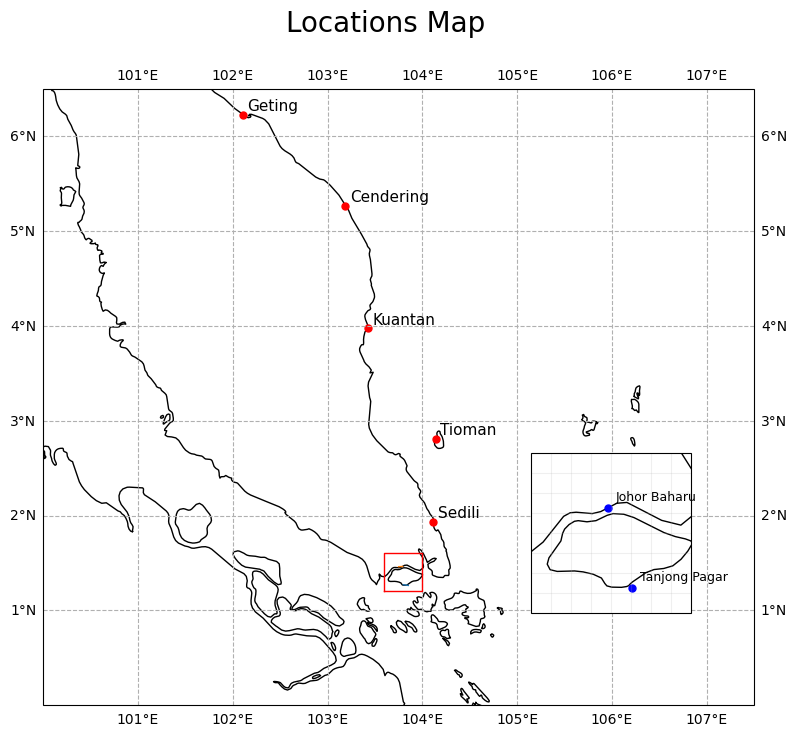
\includegraphics[width=0.75\linewidth]{Figures/locations_map.png}
        \caption{Map of tide gauges selected}
        \label{fig1}
    \end{figure*}
    \begin{paragraph} 
        \noindent In this study we aim to study the effect of two of these stochastic factors which result in the development of cold surge events on the SCS, on water levels around Peninsular Malaysia. We hope to develop a statistical framework that allows us to not only numerically quantify the effect that cold surge events have, but also identify what can be considered as `extreme' water levels. This framework allows us to gain a better understanding of floods caused by cold surge events specifically during the months of the NE monsoon, thus having real-world applications in disaster management and risk prevention measures.
    \end{paragraph}
    
    \section*{Data and Methodology}
    \addcontentsline{toc}{section}{Data and Methodology}
    \begin{paragraph}
        \noindent The term `tides' can be restricted to the vertical rise and fall of water that occurs twice a day, best observed on a coast, a breakwater or a pier \cite{Hicks2006_Tides}. In the same document, the author goes on to add that apart from terrestrial factors such as irregular ocean depths (known as `bathymetry'), interactions of ocean waters with continents, etc., unpredictable meteorological factors such as storms, typhoons, cyclones, wind surges, rain and barometric pressure can bring about major differences between the observed and the predicted tides. 
    \end{paragraph}
    \begin{paragraph}
        \noindent The usual flow of analysing water levels is in the flow chart in Figure \ref{fig2}.
        \begin{figure*}[htbp]
        \centering
        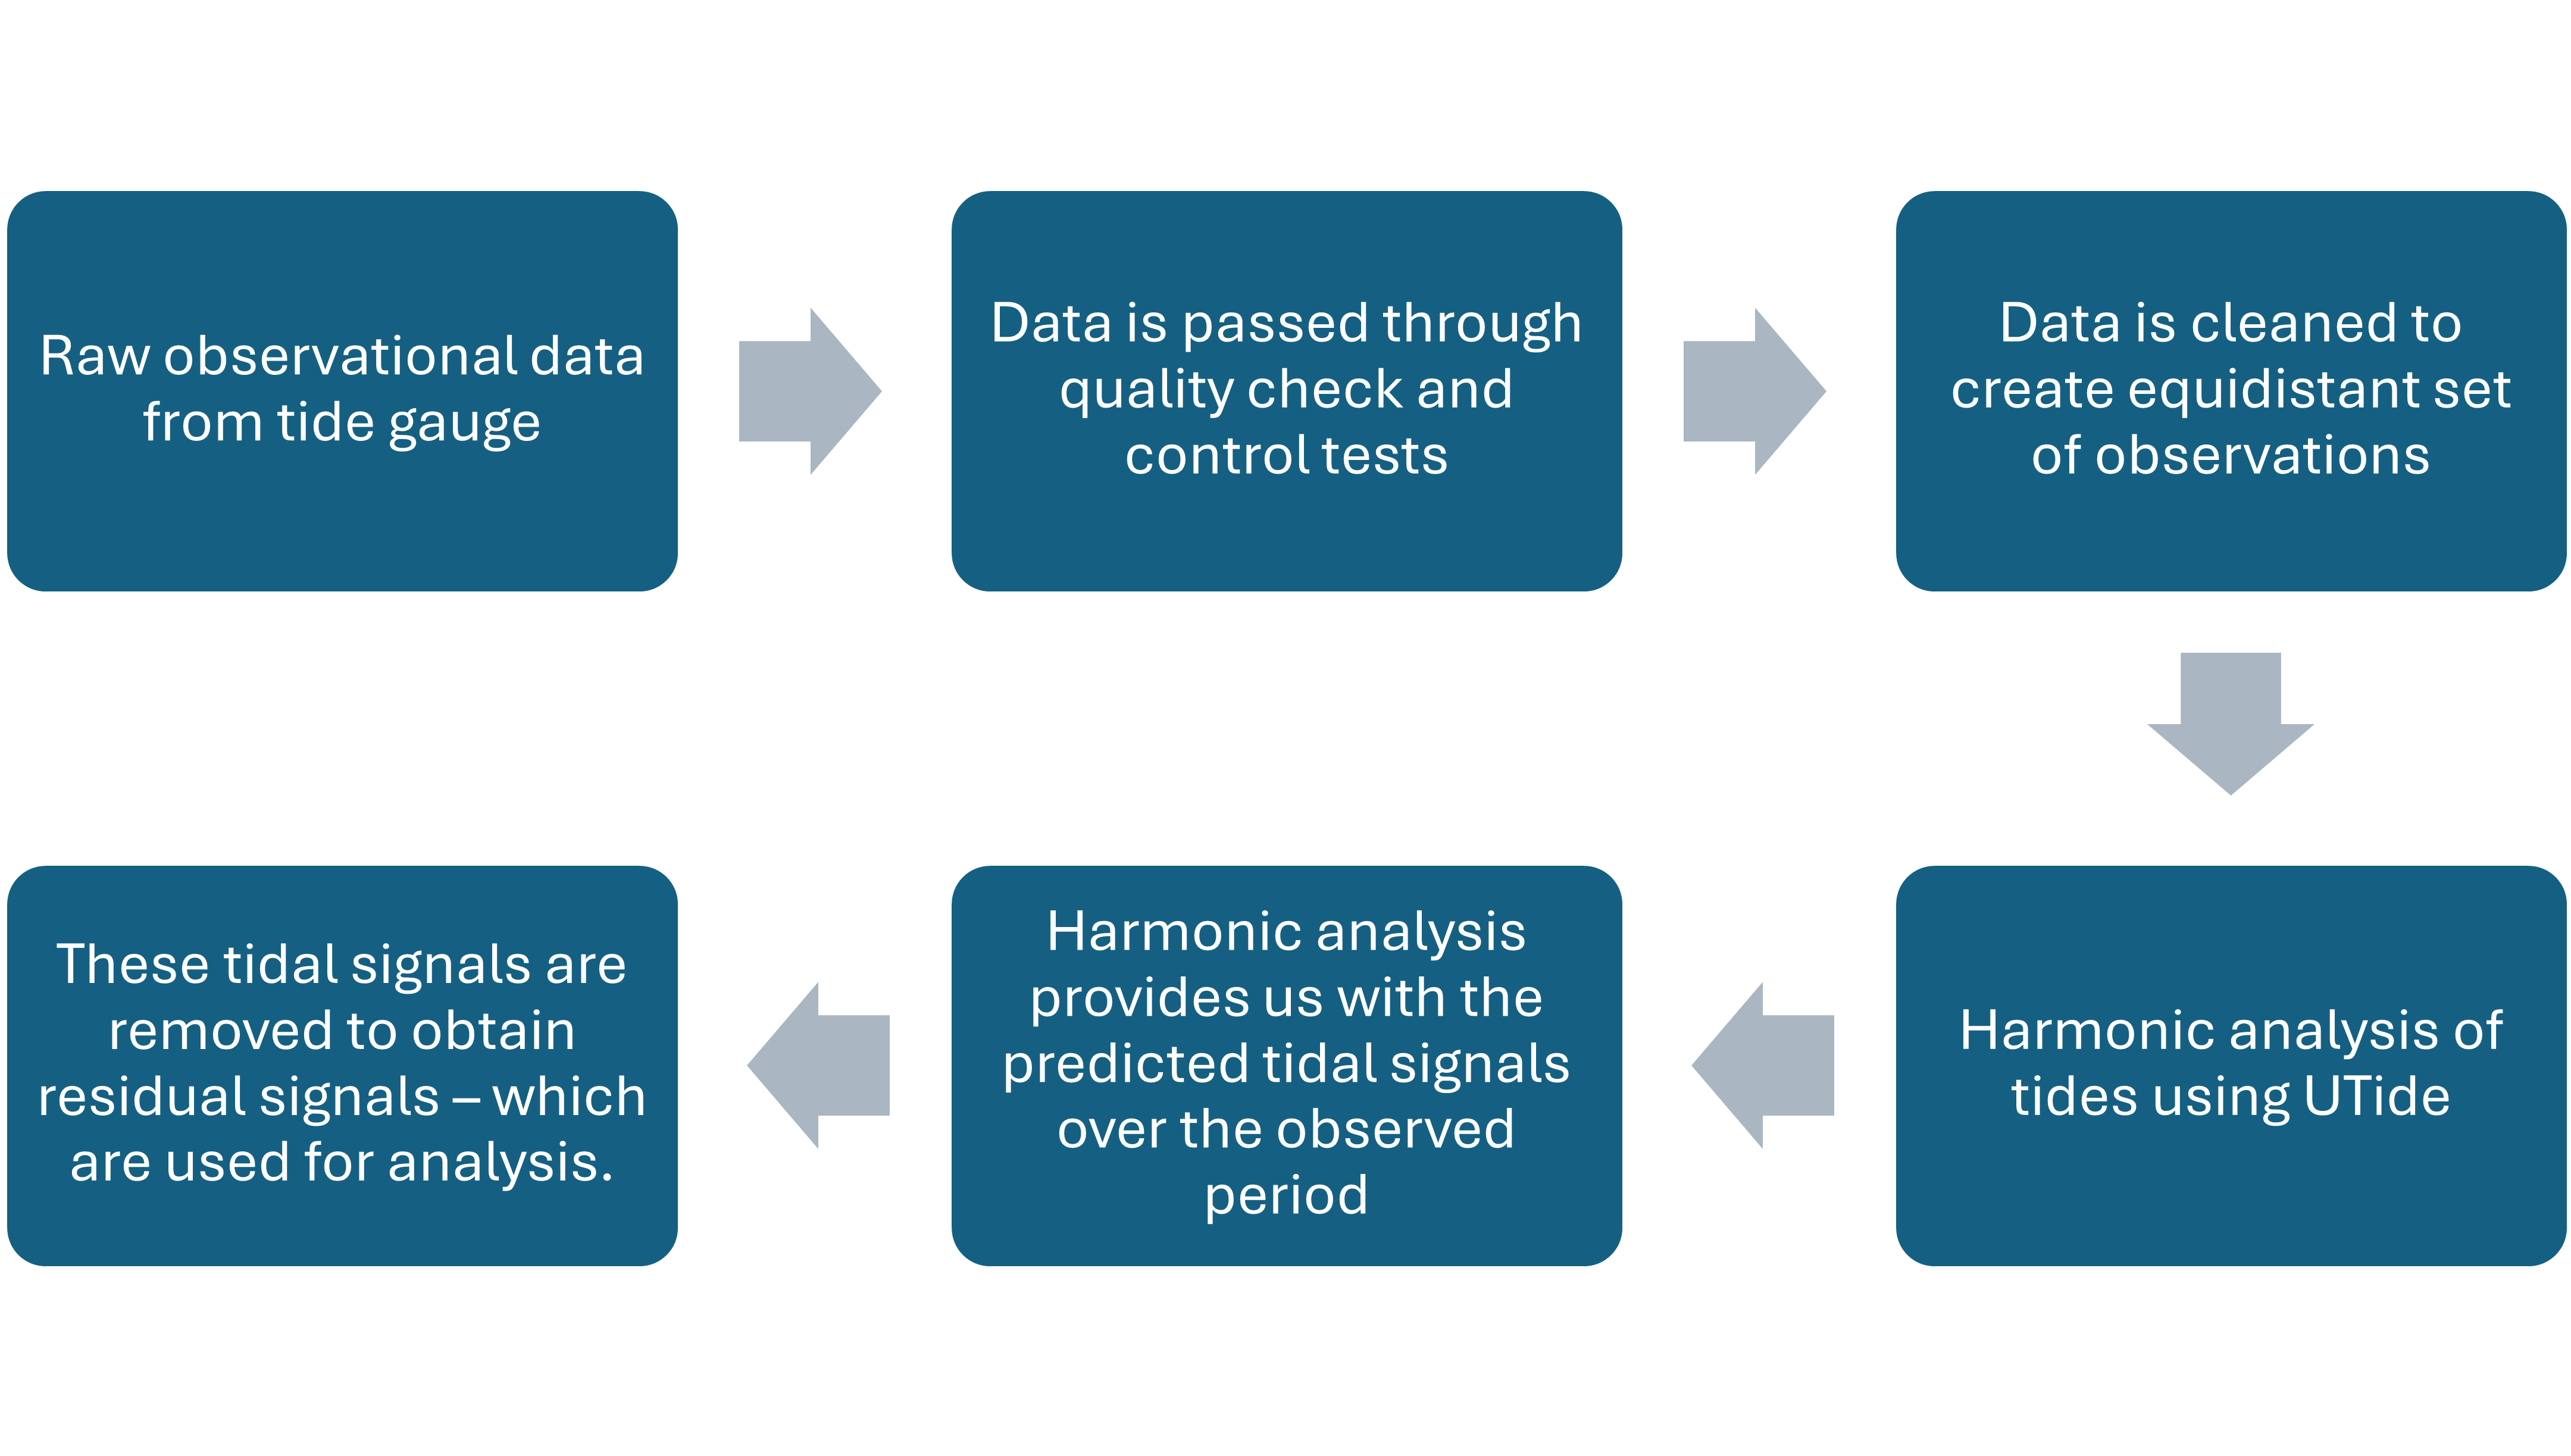
\includegraphics[width=0.75\linewidth]{Figures/Data_Cleaning.png}
        \caption{Flowchart for water level analysis}
        \label{fig2}
    \end{figure*}
        
        In order to separate the tidal signals from those caused by meteorological factors (henceforth called deterministic and stochastic signals, respectively), we use the MATLAB package UTide \cite{Codiga2011_UTIDE}. The source code for the data processing pipeline is given \href{https://github.com/shrin0811/test_stuff_for_3172}{here}. Ideally, harmonic analysis is done with data of higher frequency (for example, the Maritime Port Authority of Singapore collects data with sea level data with a six minute frequency), but due to computational and legal restrictions, could not be presented and analysed in this study.
    \end{paragraph} 
    \begin{figure*}[t]
        \centering
        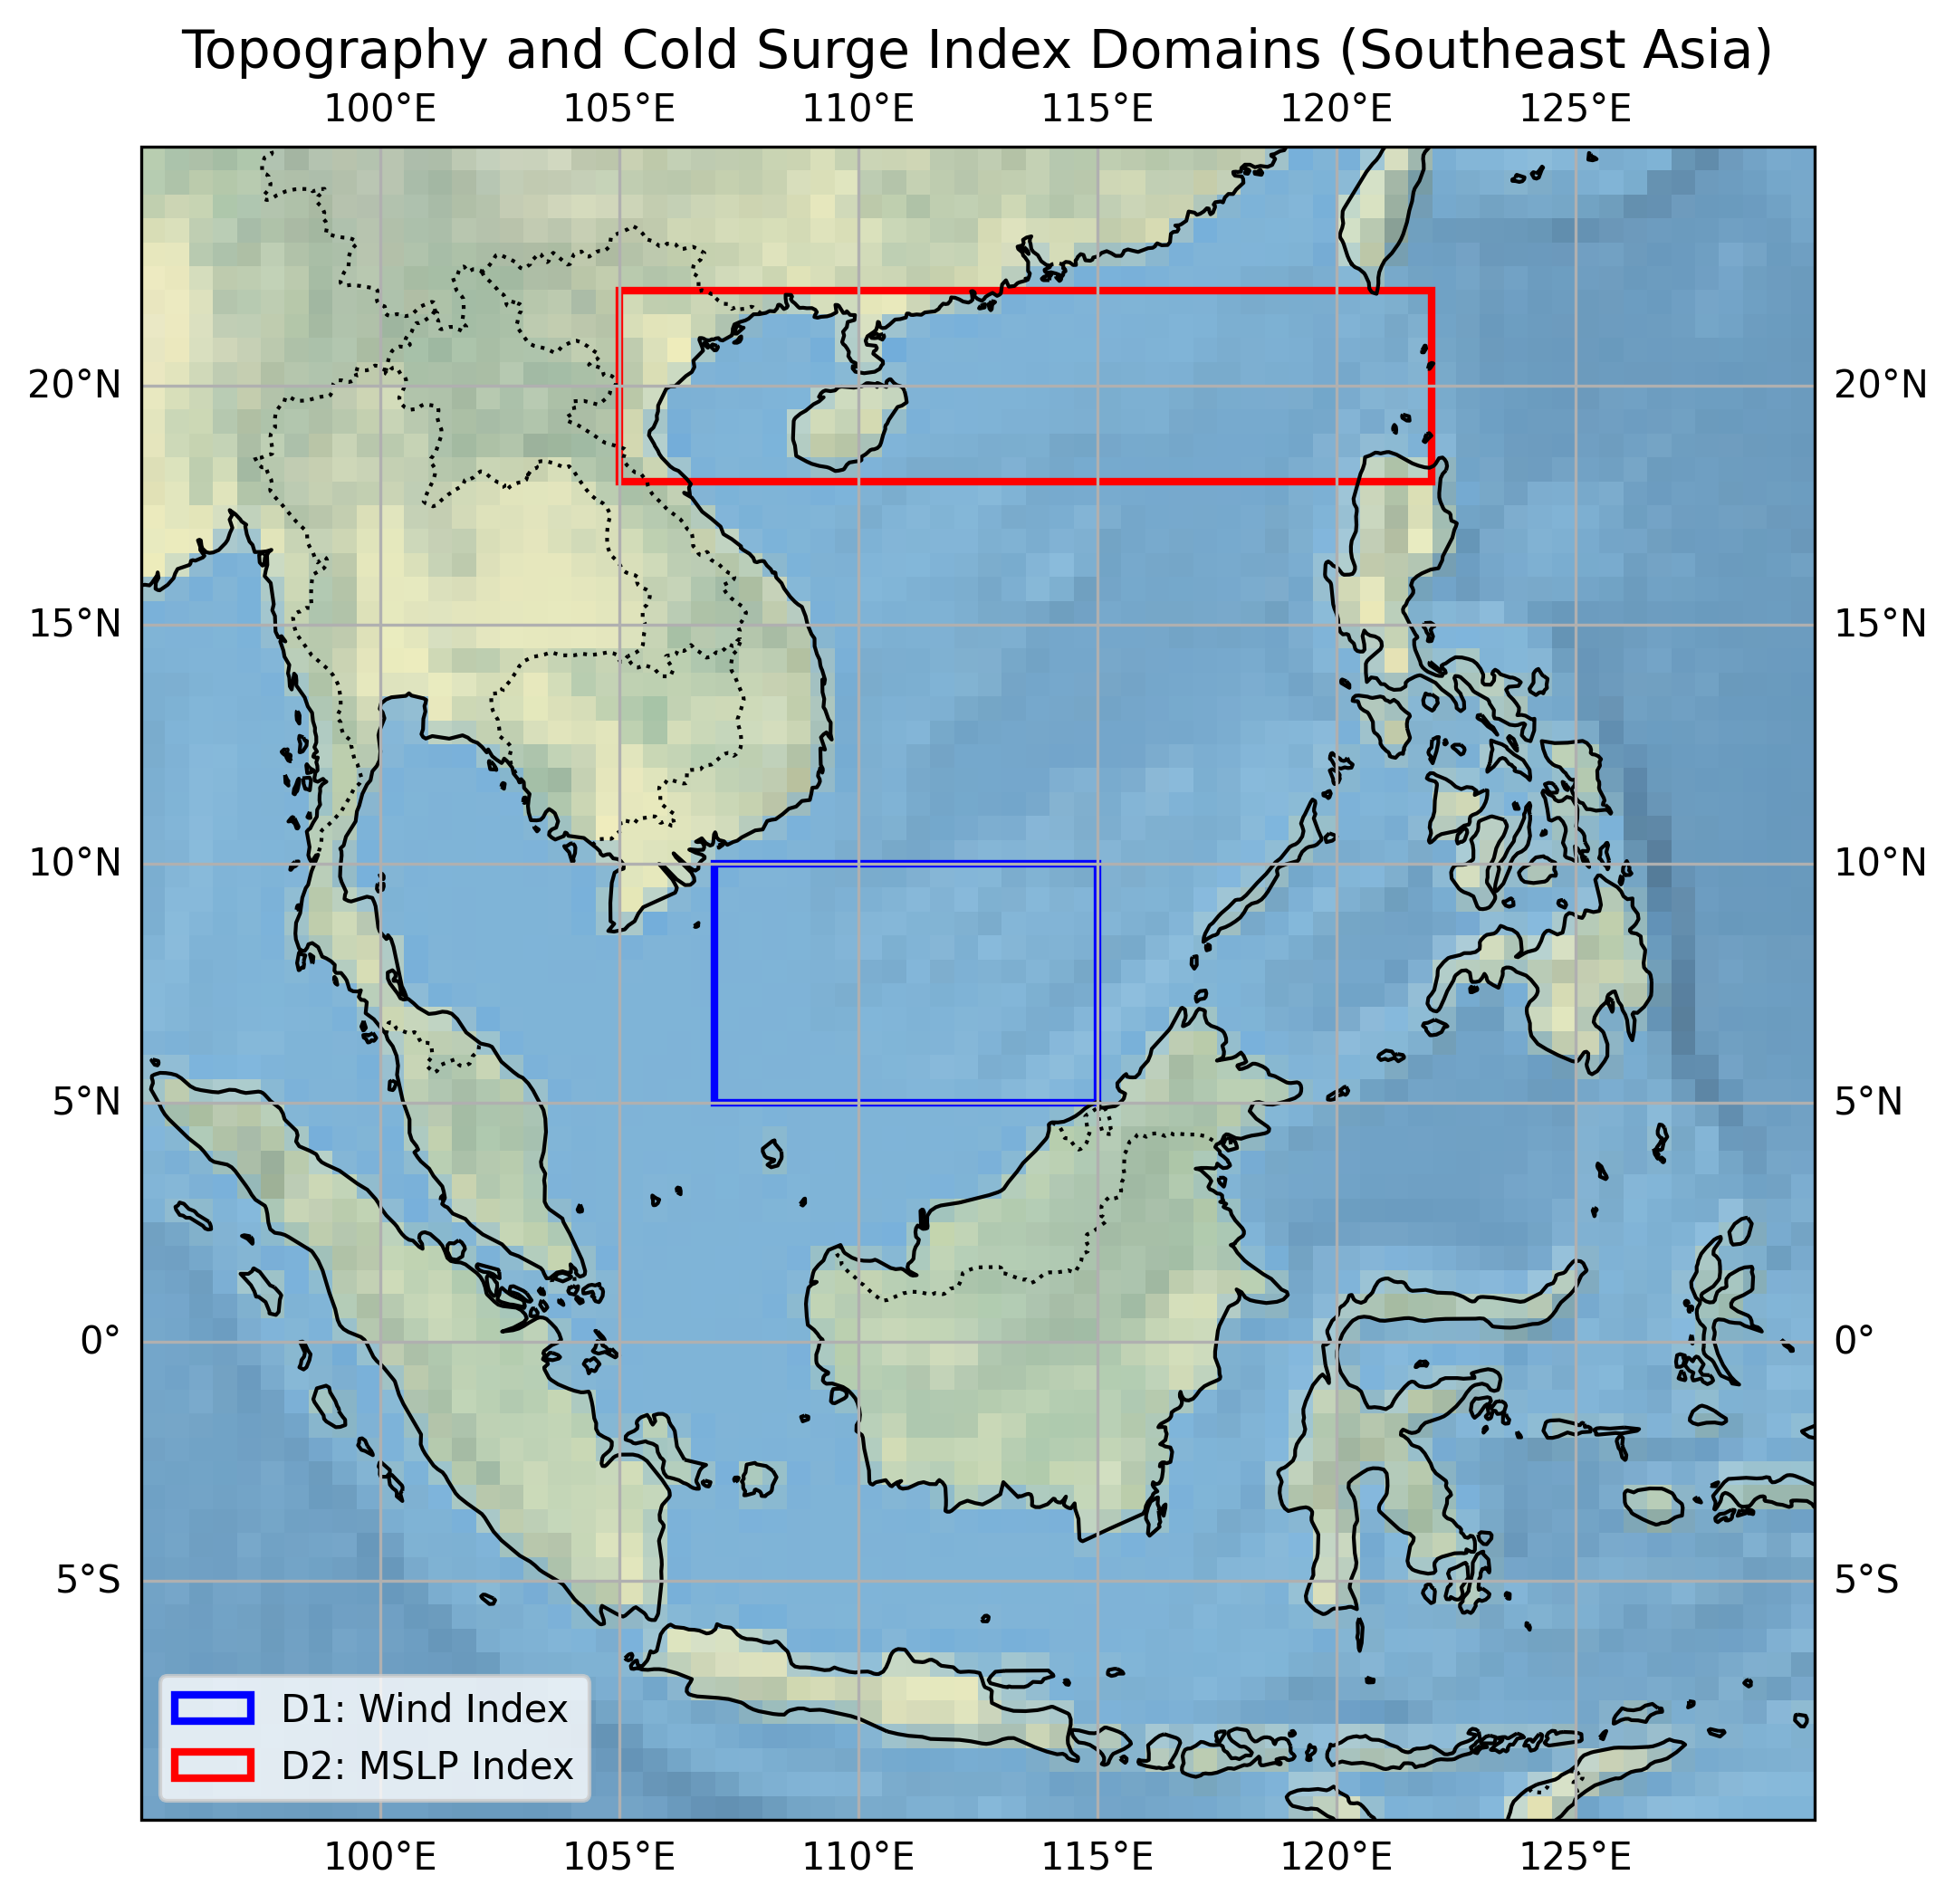
\includegraphics[width=0.7\linewidth]{Figures/D1_D2_map.png}
        \caption{Regions of the South China Sea that were used to calculate and flag surge days}
        \label{fig3}
    \end{figure*}
    \begin{paragraph}
        \noindent The general formula \cite{Tkalich2013_StormSurge} used for calculating water levels at a given time t is as follows: 
        \begin{align*}
            T(t) = P(t) +R(t)
        \end{align*}
        where T(t) is the total water level, P(t) is the predicted water level calculated by UTide \cite{Codiga2011_UTIDE} based on a unified tidal equation, corrected for satellite positions and Greenwich phase lags and R(t) is the residual water level caused by meteorological and weather events. Note that the daily still has hourly frequency. As we are looking for high residual water levels, we take the  maximum of each of the 24 data points (corresponding to each hour in the each day) of each day, thus compiling a list of daily maximum values across the selected time period.
    \end{paragraph}  
    
    \begin{paragraph}
        \noindent We analysed seven tide gauges along the eastern coast of Malaysia and Singapore, that directly face the South China Sea as shown in Figure 1. Moreover, these seven tide gauges have some of the longest records in Southeast Asia, with more than 25 years of data available, and a completion rate of above 95\% (\cite{Koh2024_TideSurge}). A summary of these statistics is shown in Table \ref{table_1} below. 
    \end{paragraph}


    \begin{table*}[htbp]
     \begin{center}
        \begin{tabular}{||c c c||} 
         \hline
         Location & Lat/Lon & Range of Data Available \\ [0.5ex] 
         \hline\hline
         Cendering & $5.265^\circ N$/$103.187^\circ E$ & 1984-2015 \\ 
         \hline
         Geting & $3.975^\circ N$/$103.43^\circ E$ & 1986-2015 \\
         \hline
         Kuantan & $5.265^\circ N$/$103.187^\circ E$ & 1983-2015 \\
         \hline
         Johor Baharu & $1.462^\circ N$/$103.792^\circ E$ &  1983-2013 \\
         \hline
         Sedili & $1.932^\circ N$/$104.115^\circ E$ & 1986-2015 \\
         \hline
         Tioman & $2.807^\circ N$/$104.14^\circ E$ & 1985-2015  \\
         \hline
         Tanjong Pagar & $1.262^\circ N$/$103.853^\circ E$ &  1984-2018 \\ [1ex]
         \hline
        \end{tabular}
        \caption{Summary of the tide gauge stations used}
        \label{table_1}
        \end{center}
        
    \end{table*}

    \begin{paragraph}
        \noindent In order to develop the dependent variables of the model, we used ERA5 re-analysis data \cite{Hersbach_2020} of wind speeds in the domain $5^\circ - 10^\circ N$ and $107^\circ - 115^\circ E$, and mean sea level pressure (MSLP) in the domain $18^\circ - 22^\circ N$ and $105^\circ - 122^\circ E$. This is in line with the definition of a cold surge event that was used for Singapore's latest climate report, which was further based upon thresholds established in \cite{Lim2017_MonsoonRainfall}. The two domains are clearly represented in Figure \ref{fig3}.
    \end{paragraph}
    
    \begin{paragraph}
        \noindent Cold surges indices in Singapore's third climate change study \cite{NEA_2024} are defined based on area-weighted averages of the vertical and horizontal components of wind speeds (in m/s), and MSLP (in Pa). These averages were calculated using Climate Data Operators \cite{Schulzweida2023_CDO} a command-line software suite that easily allow us to manipulate large-scale climate and NWP datasets. For a CS event to be flagged, wind equaling 0.75 standard deviations above the long-term mean over the months of November, December, January and February (NDJF) is taken into consideration. A surge day is flagged when the wind direction is northerly or northeasterly with a speed above the threshold, providing MSLP is above 1020 hPa anywhere within the domain D2 \cite{Lim2017_MonsoonRainfall}, \cite{NEA_2024}. Figures showing the distribution of the area-weighted averages for both components can be found in Appendix A.
    \end{paragraph}

    \begin{paragraph}
        \noindent As the aim of this study is to analyse the effect of CS events on Peninsular Malaysia, and not recreate the exact tidal shape, we put considerable effort into deciding statistical frameworks which would allow us to balance statistical accuracy, limited granularity and climatic variability. As the range of wind speeds and MSLP differs by a power of $10^{4}$ in their respective SI units, we used the Z-score-normalisation technique such that the entire distribution has a mean of 0, and a standard deviation of 1. These normalised datasets were used as the dependent variables to train each model. Moreover, we took a common timeframe among all seven stations (1990 - 2013), to not only ensure that the period being analysed is close to the recommended minimum of 30 years \cite{Rasmussen2018_SeaLevelImpacts}, but also to prevent the effect of differing large-scale climate events. For example, Johor Baharu has records till 2013, while Tanjong Pagar has records till 2018. As per the ENSO-MEI index \cite{Wolter2018_MEI}, NDJF across 2013 was in a weaker La-Ni\~na phase (while some months were not in either phase), while the same period in 2018 was in a stronger La-Ni\~na phase. Studies \cite{Dieng2014}, \cite{Han_Huang_2008} have shown that water levels are generally lower during stronger La-Ni\~na (cooler) phases and higher during strong El-Ni\~no phases, thus justifying our choice to ensure that the model is trained on datasets of equal length for all seven tide gauges.
    \end{paragraph}

    \begin{figure*}[htbp]
        \centering
        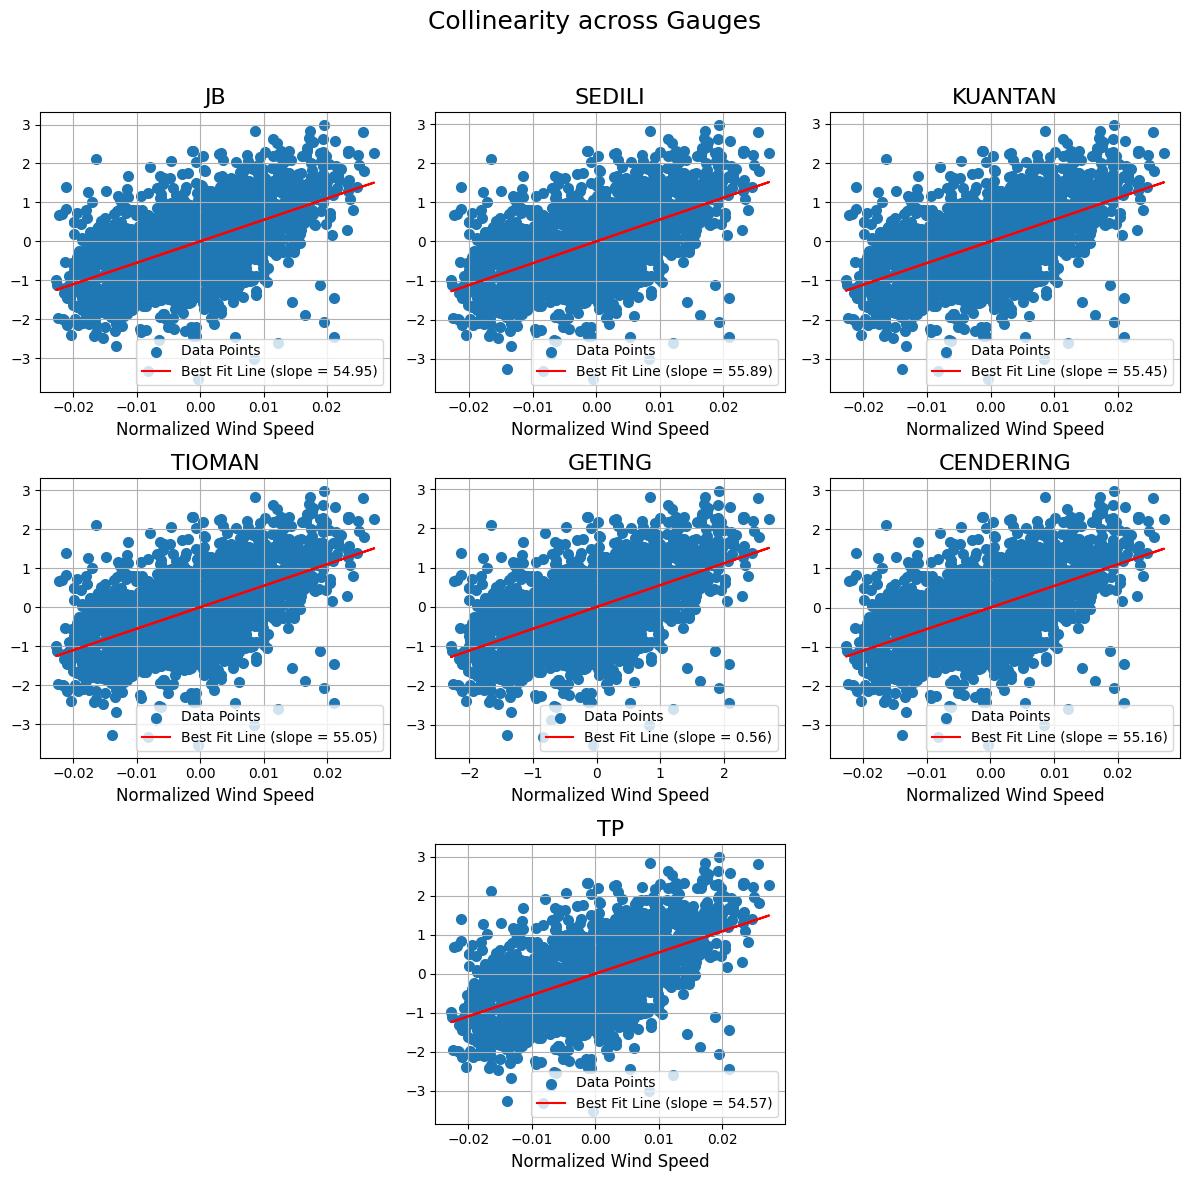
\includegraphics[width=\linewidth]{Figures/collinearity.png}
        \caption{Collinearity between the independent variables for the model}
        \label{fig4}
    \end{figure*}

    \begin{paragraph}
        \noindent Apart from using linear, quadratic and cubic polynomial fits for the datasets, we also used L1 and L2 regularisation techniques (commonly known as lasso and ridge regression) to fit the data. These techniques were added due to the observed collinearity (Figure) between the normalised wind speed and MSLP datasets for each location, shown in Figure \ref{fig4}. After training the model on datasets between 1990 - 2013, we checked for R\textsuperscript{2} values as measure of how well the model explains variance, and the mean-absolute error for each model. As is the standard for most meteorological studies, we also studied the behaviour of the best-forming model for records before 1990 and after 2013 for each station, intersecting with the days determined to be surge days between those time periods, which allows us to determine the level for `extreme' water levels that could potentially lead to floods in low-lying areas. 
    \end{paragraph}

    \newpage 
    \newpage
    \section*{Results and Discussion}
    \addcontentsline{toc}{section}{Results and Discussion}

        \begin{figure*}[htbp]
        \centering
        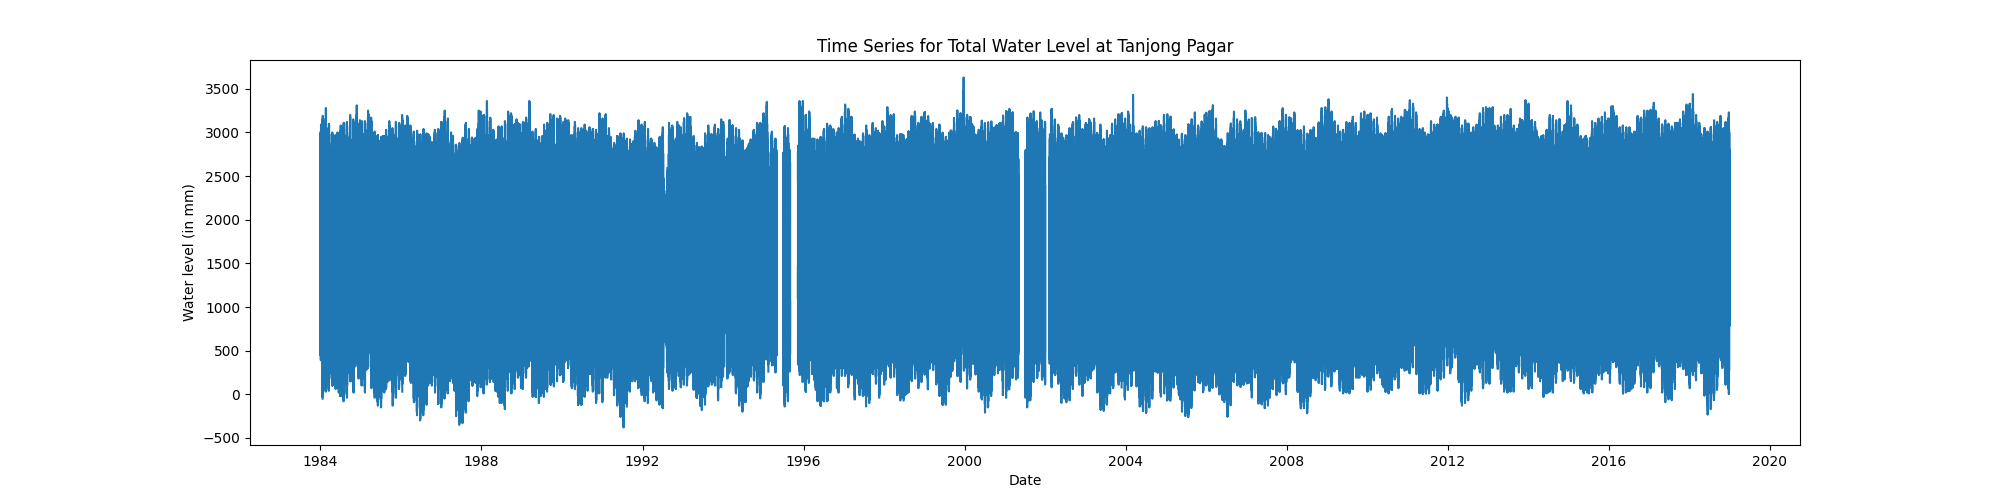
\includegraphics[width=\linewidth]{Figures/Time Series for Total Water Level at Tanjong Pagar.png}
        \caption{Mean Sea Level at Tanjong Pagar station}
        \label{total_tp}
    \end{figure*}

            \begin{figure*}[htbp]
        \centering
        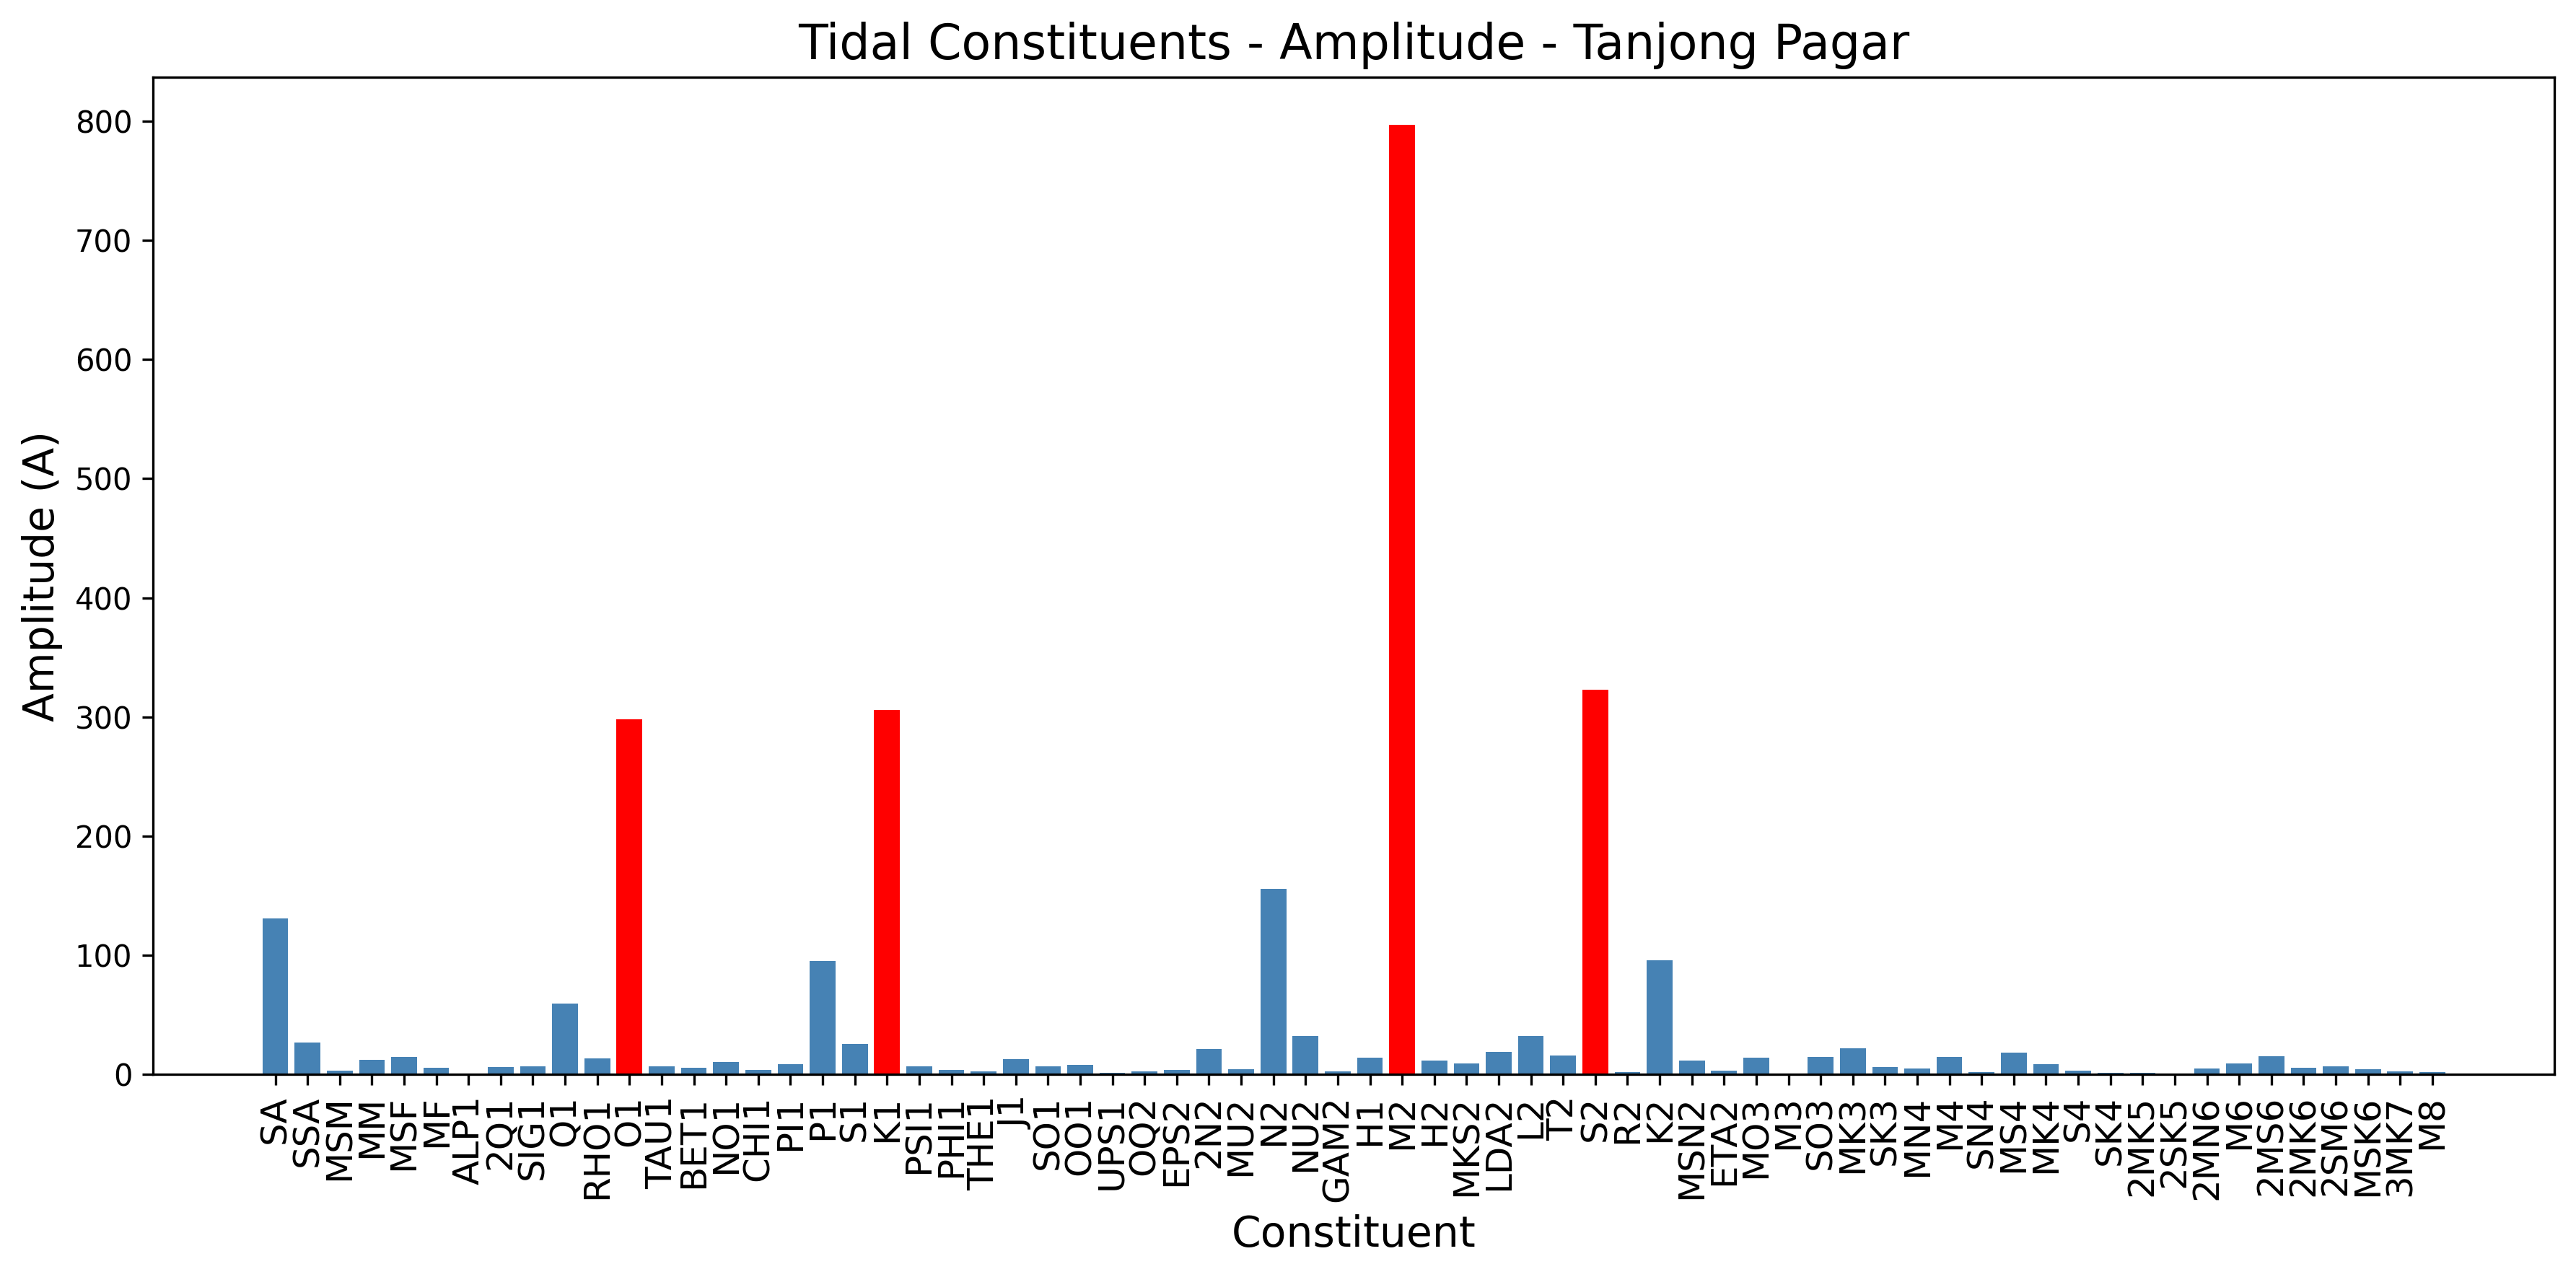
\includegraphics[width=\linewidth]{Figures/TP_Constituents.png}
        \caption{Tidal Constituents for Tanjong Pagar}
        \label{tp_cons}
    \end{figure*}

    \begin{figure*}[htbp]
        \centering
        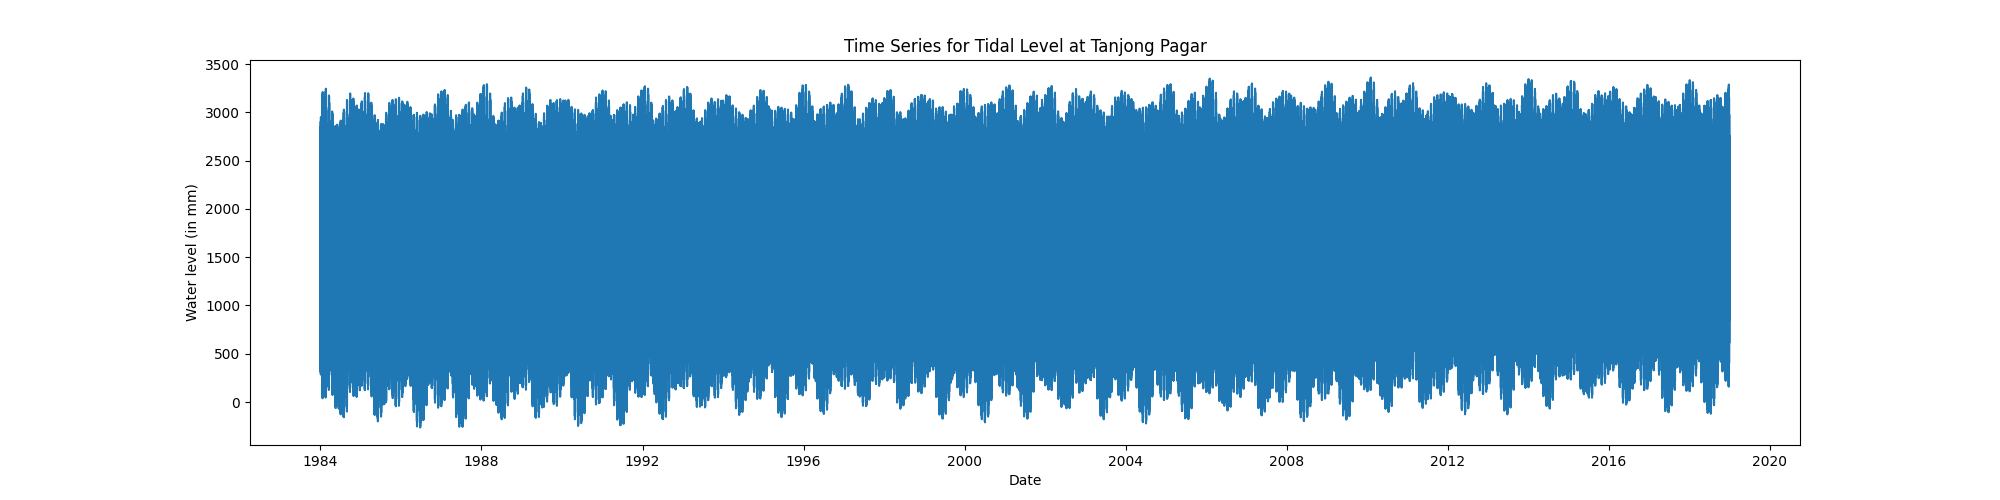
\includegraphics[width=\linewidth]{Figures/Time Series for Tidal Level at Tanjong Pagar.png}
        \caption{Predicted Tidal Levels at Tanjong Pagar station}
        \label{tidal_tp}
    \end{figure*}

    \begin{figure*}[htbp]
        \centering
        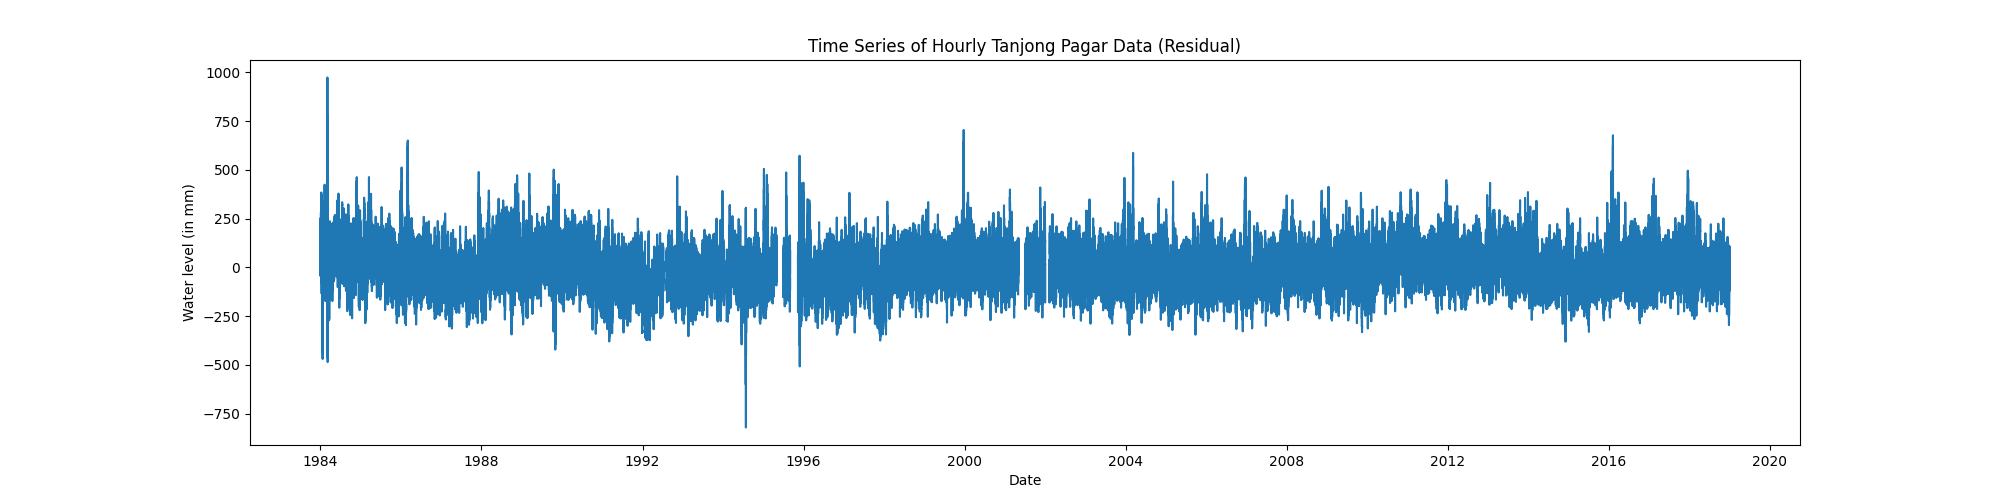
\includegraphics[width=\linewidth]{Figures/Time Series of Hourly Tanjong Pagar Data (Residual).png}
        \caption{Residual (stochastic) Water Levels at Tanjong Pagar Station}
        \label{residual_tp}
    \end{figure*}
    
        \begin{table*}[b]
\centering
\caption{R\textsuperscript{2} and MAE values for different regression models across locations}
\begin{adjustbox}{width=\textwidth}
\begin{tabular}{lcccccc}
\toprule
\textbf{Model} & \textbf{JB} & \textbf{Sedili} & \textbf{Kuantan} & \textbf{Tioman} & \textbf{Geting} & \textbf{Cendering} \\
\midrule
Linear & 0.253 / 77.73 & 0.250 / 89.15 & 0.245 / 82.93 & 0.243 / 81.87 & 0.180 / 123.28 & 0.260 / 89.22 \\
Quadratic & 0.289 / 76.21 & 0.280 / 87.39 & 0.281 / 80.73 & 0.279 / 79.57 & 0.195 / 121.78 & 0.290 / 87.31 \\
Cubic & 0.296 / 76.11 & 0.284 / 87.22 & 0.286 / 80.54 & 0.285 / 79.50 & 0.200 / 121.42 & 0.294 / 87.19 \\
Ridge & 0.225 / 78.98 & 0.215 / 90.45 & 0.225 / 83.92 & 0.221 / 83.22 & 0.180 / 123.28 & 0.242 / 90.38 \\
Ridge ($\alpha=0.1$) & 0.246 / 77.90 & 0.242 / 89.19 & 0.241 / 83.14 & 0.238 / 82.27 & 0.180 / 123.28 & 0.256 / 89.46 \\
Ridge (1000 iter) & 0.225 / 78.98 & 0.215 / 90.45 & 0.225 / 83.92 & 0.221 / 83.22 & 0.180 / 123.28 & 0.242 / 90.38 \\
Lasso & 0.216 / 79.36 & 0.205 / 90.98 & 0.219 / 84.21 & 0.214 / 83.53 & 0.180 / 123.29 & 0.237 / 90.75 \\
Lasso ($\alpha=0.1$) & 0.242 / 78.07 & 0.242 / 89.18 & 0.235 / 83.40 & 0.233 / 82.56 & 0.180 / 123.28 & 0.252 / 89.73 \\
\bottomrule
\end{tabular}
\label{table_2}
\end{adjustbox}
\end{table*}

    \begin{paragraph}
        \noindent We begin by first presenting the results obtained after using UTide \cite{Codiga2011_UTIDE} on all seven locations. Figures \ref{total_tp}, \ref{tp_cons}, \ref{tidal_tp} and \ref{residual_tp} only represent the results for the Tanjong Pagar station, while the remaining are presented in Appendix B. 
        Among astronomic principal and major tidal harmonics (for Tanjong Pagar station) we note the following diurnal amplitudes M2 = 79.70 cm, S2 = 32.30 cm, K1 = 30.60 cm, O1 = 29.80 cm - the primary diurnal amplitudes. We also observed a comparable amplitude of annual SA = 13.10 cm and semiannual SSA = 2.68 cm, which coincides with the observed literature that Singapore has a mixture of the diurnal and semi-diurnal tidal regimes. \cite{Maren_Gerritsen_2012}
    \end{paragraph}


    %% add the water level diagrams and constituents here

    \begin{paragraph}
        \noindent The Venn diagrams (Figure \ref{tp_venn}) analyzing the relationship between the days with surges in water levels and the days with high water levels for the various percentiles give a juxtaposed view with the surge events and water levels. Viewed through sensitivity and specificity lens, a distinct trade-off shows. At the lower percentiles (between 50th – 75th), the overlap between surge days and high water level days is larger which hints at higher sensitivity – capturing most actual surges, many surge days are inaccurately captured. These thresholds also include a large volume of non-surge days that results in lower specificity leading to more false positives. As the threshold increases towards 95th and 99th percentiles the overlap decreases significantly. This indicates higher specificity with fewer false positives but achieves lower sensitivity where most surge days are missed. Therefore, most of the upper percentiles would be conservative and accurate while detecting extreme events, but in reality would capture very few real surges. Therefore, a balance between the specificity and the sensitivity must be achieved after we select our best-performing model. The venn diagrams for the remaining stations are provided in Appendix C.
    \end{paragraph}

    \begin{figure*}[htbp]
        \centering
        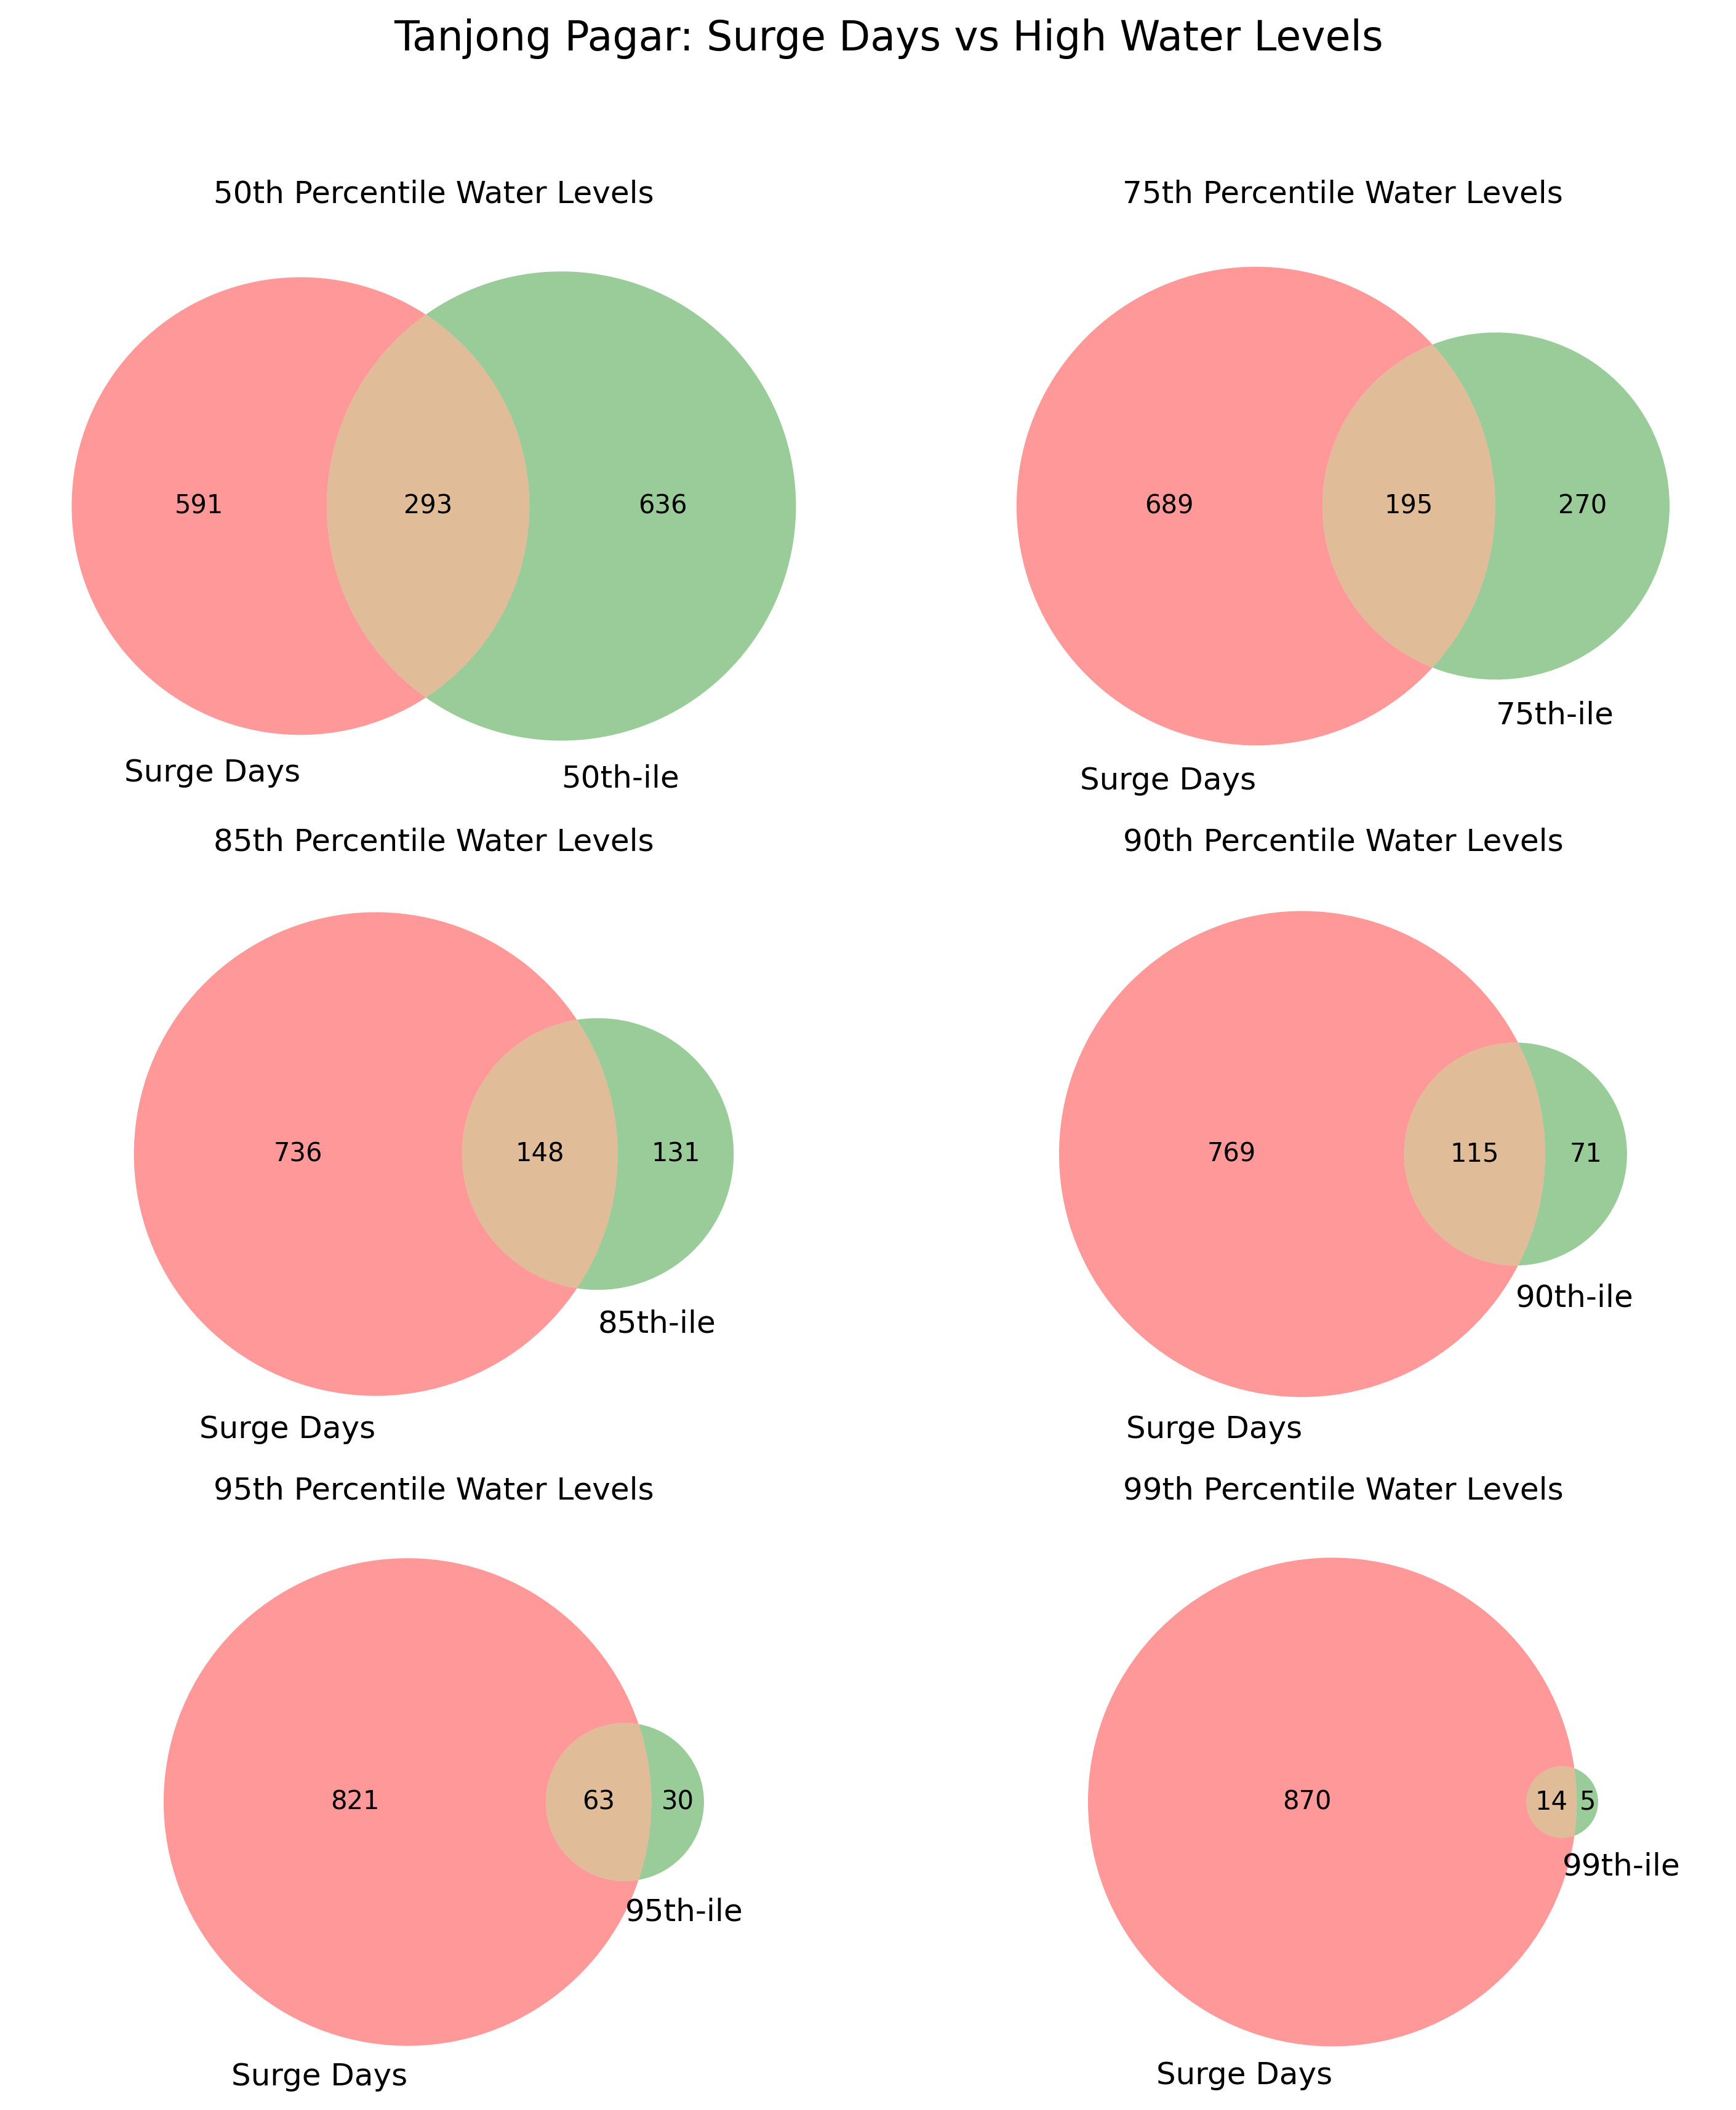
\includegraphics[width=\linewidth]{Figures/TP_venn.png}
        \caption{Venn Diagrams showing the intersection of water levels with surge days for different thresholds}
        \label{tp_venn}
    \end{figure*}

    \begin{paragraph}
        \noindent We evaluated the performance of multiple regression models such as linear, quadratic and cubic polynomials, along with ridge and lasso regression models to explore the relation between wind speeds and MSLP, with residual water levels. Model accuracy assessment was performed using R\textsuperscript{2} and mean absolute error (MAE) across the seven locations. A primary metric of MAE was chosen due to the ease of interpretability, and in the context of outliers, extreme value prediction had relevance. We made a conscious choice to not use the RMSE values for this particular climate model. RMSE is a function of three characteristics of a set of errors, and varies within the variability within the distribution of the error magnitudes and square root of the number of errors (\cite{Willmott2005_MAE}). Therefore, the MAE is a better predictor of average error, thus allowing better comparisons of model performance.
    \end{paragraph}

    \newpage 
    \begin{figure*}[htbp]
        \centering
        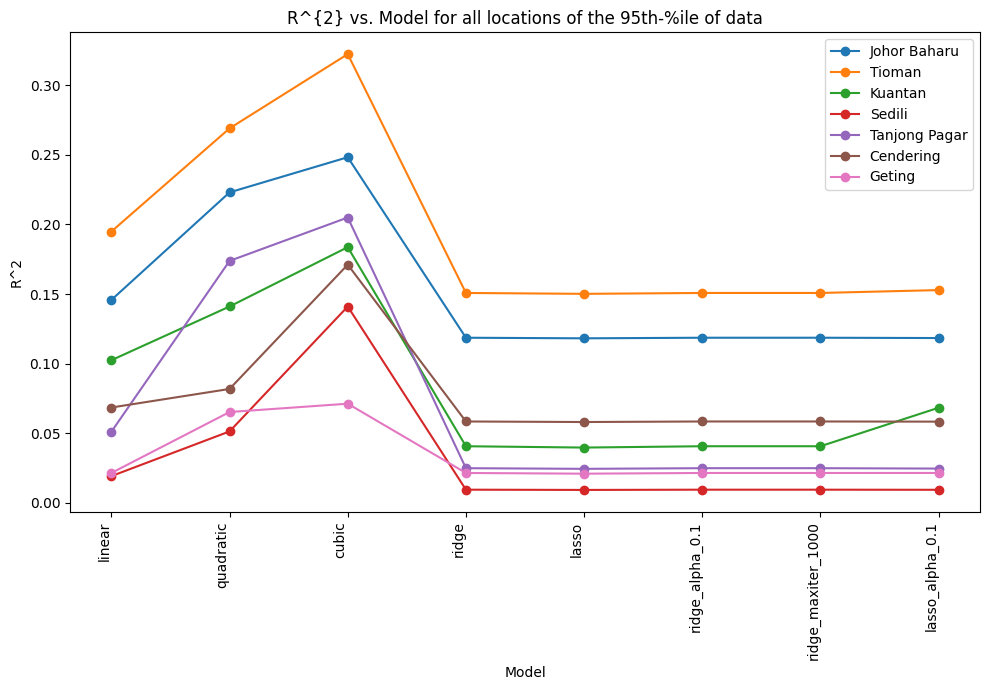
\includegraphics[width=0.8\linewidth]{Figures/R^2_all_locs_95th.png}
        \caption{Mean Absolute Error for Tanjong Pagar Station across various regression models}
        \label{r^2_score}
    \end{figure*}

        \begin{figure*}[htbp]
        \centering
        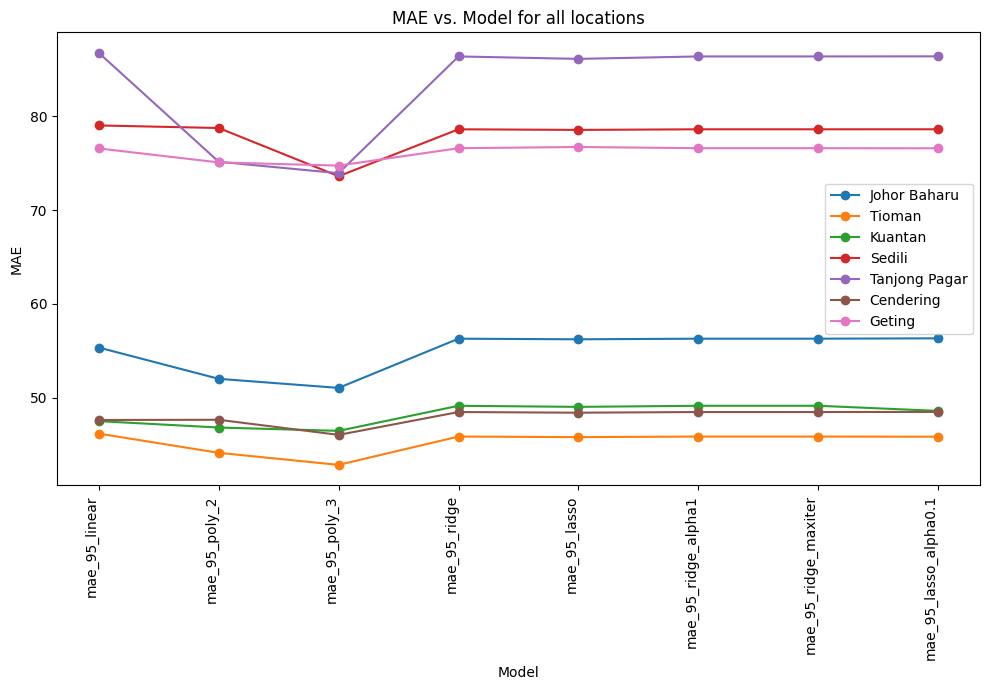
\includegraphics[width=0.8\linewidth]{Figures/MAE_all_locations.png}
        \caption{Mean Absolute Error for Tanjong Pagar Station across various regression models}
        \label{mae_all}
    \end{figure*}

    \begin{figure*}[htbp]
        \centering
        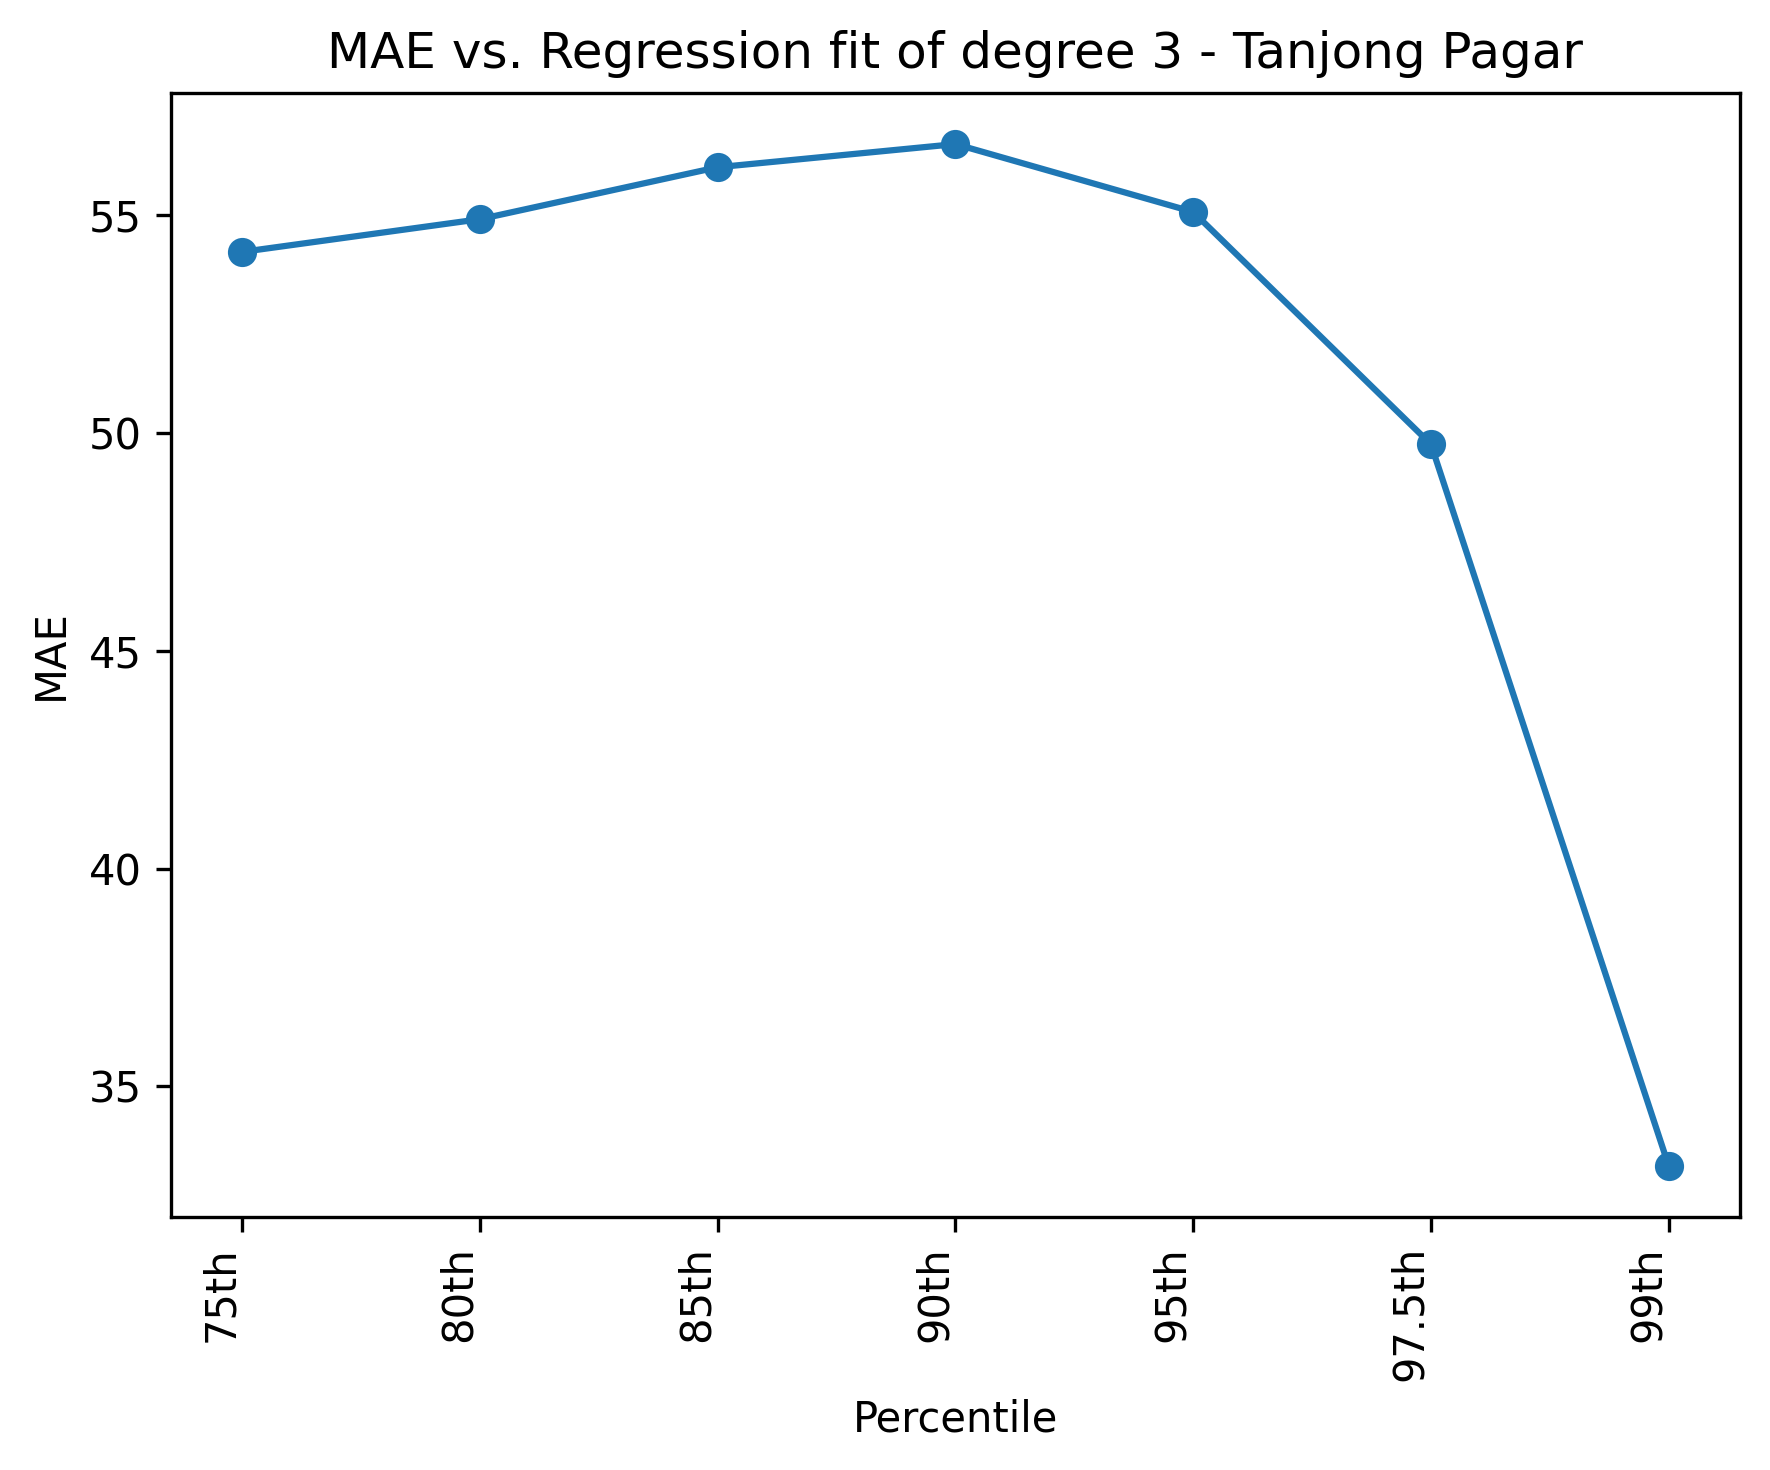
\includegraphics[width=0.7\linewidth]{Figures/MAE_TP_diff_percentile.png}
        \caption{Mean Absolute Error for Tanjong Pagar Station across different benchmarks of water levels}
        \label{mae_tp}
    \end{figure*}

    \newpage
        \begin{paragraph} 
        \noindent Although cubic models were repeatedly the best-performing models among those tested, R\textsuperscript{2} values were persistently low across all models and sites (generally less than 0.30). This indicates that in a substantial portion of the variance of the residual maxima, the predictors fail to capture most of the variance. We hypothesize that the generally low R\textsuperscript{2} could be the complex nature of other factors that influence the processes of residual water levels at the seven locations such as, the limited size of the dataset, the low number of predictors (from a statistical standpoint), the geometry of the coastline, local bathymetric features or the duration and direction of the wind (from a meteorological standpoint). Therefore, while it suggests that the model has some predictive skill, assuming generally low R\textsuperscript{2} may be an indicator that the input data needs to be more comprehensive.
    \end{paragraph}


    \begin{paragraph}
        \noindent Out of all the regression models examined, the polynomial of degree three excelled in all seven locations in R\textsuperscript{2} and mean absolute error (MAE) of prediction when compared to others, as observed in Table \ref{table_2}. In particular, the cubic model yielded the highest R\textsuperscript{2} values and the least MAE at each location, thus demonstrating more accuracy than linear, quadratic, ridge, and lasso models. These results imply that the polynomial of degree three offers the best solution for the data's nonlinear relationships throughout the entire dataset and across percentiles. This is further corroborated by Figure \ref{r^2_score} and \ref{mae_all}, along with the comparison with observed 99th-percentile data (by definition these can be considered as sea-level anomalies) in Figure \ref{99_poly3_fit}. Improvement over less complex models (linear and quadratic) suggest that higher-order terms add value, while the advantage over ridge and lasso suggests greater flexibility of the cubic functions does not result in overfitting. Figure \ref{mae_tp}, further shows that error drastically reduces as we move to higher percentiles, but as we observed before, choosing the highest percentile to be the threshold for `extreme' tides may prove counter-productive to correlation with CS events.
    \end{paragraph}

 

    \begin{table*}[htbp]
\centering
\begin{tabular}{|l|l|r|r|r|r|}
\hline
\textbf{Station} & \textbf{Variable} & \textbf{$x$} & \textbf{$x^{2}$} & \textbf{$x^{3}$} & \textbf{intercept} \\
\hline
Johor Baharu        & wind & 2.0154e-05 & 7.5297e-08 & -7.3282e-11 & -0.00463 \\
Johor Baharu        & msl  & 3.7196e-03 & 1.9545e-06 & -2.4606e-09 & -0.56519 \\
\hline
Sedili    & wind & 2.7053e-05 & 4.8680e-08 & -6.8408e-11 & -0.00350 \\
Sedili    & msl  & 4.1536e-03 & -1.3417e-06 & -1.8914e-09 & -0.36560 \\
\hline
Kuantan   & wind & 2.8542e-05 & 1.8067e-08 & -1.3630e-12 & -0.00319 \\
Kuantan   & msl  & 4.1165e-03 & -1.1318e-06 & 9.5411e-10 & -0.37868 \\
\hline
Tioman    & wind & 2.6677e-05 & 3.3382e-08 & -8.3218e-12 & -0.00303 \\
Tioman    & msl  & 4.0940e-03 & -2.1291e-06 & 4.1233e-09 & -0.33752 \\
\hline
Geting    & wind & 2.2030e-03 & 1.1046e-06 & -3.0707e-09 & -0.22195 \\
Geting    & msl  & 3.3377e-03 & -2.0176e-06 & -2.2008e-09 & -0.22171 \\
\hline
Cendering & wind & 2.8258e-05 & 1.8937e-08 & -2.7324e-11 & -0.00296 \\
Cendering & msl  & 4.0574e-03 & -1.9599e-06 & 1.6664e-09 & -0.34217 \\
\hline
\end{tabular}
\caption{Coefficients and intercepts for wind and MSL across stations for the cubic fit}
\label{table_3}
\end{table*}


            \begin{figure*}[htbp]
        \centering
        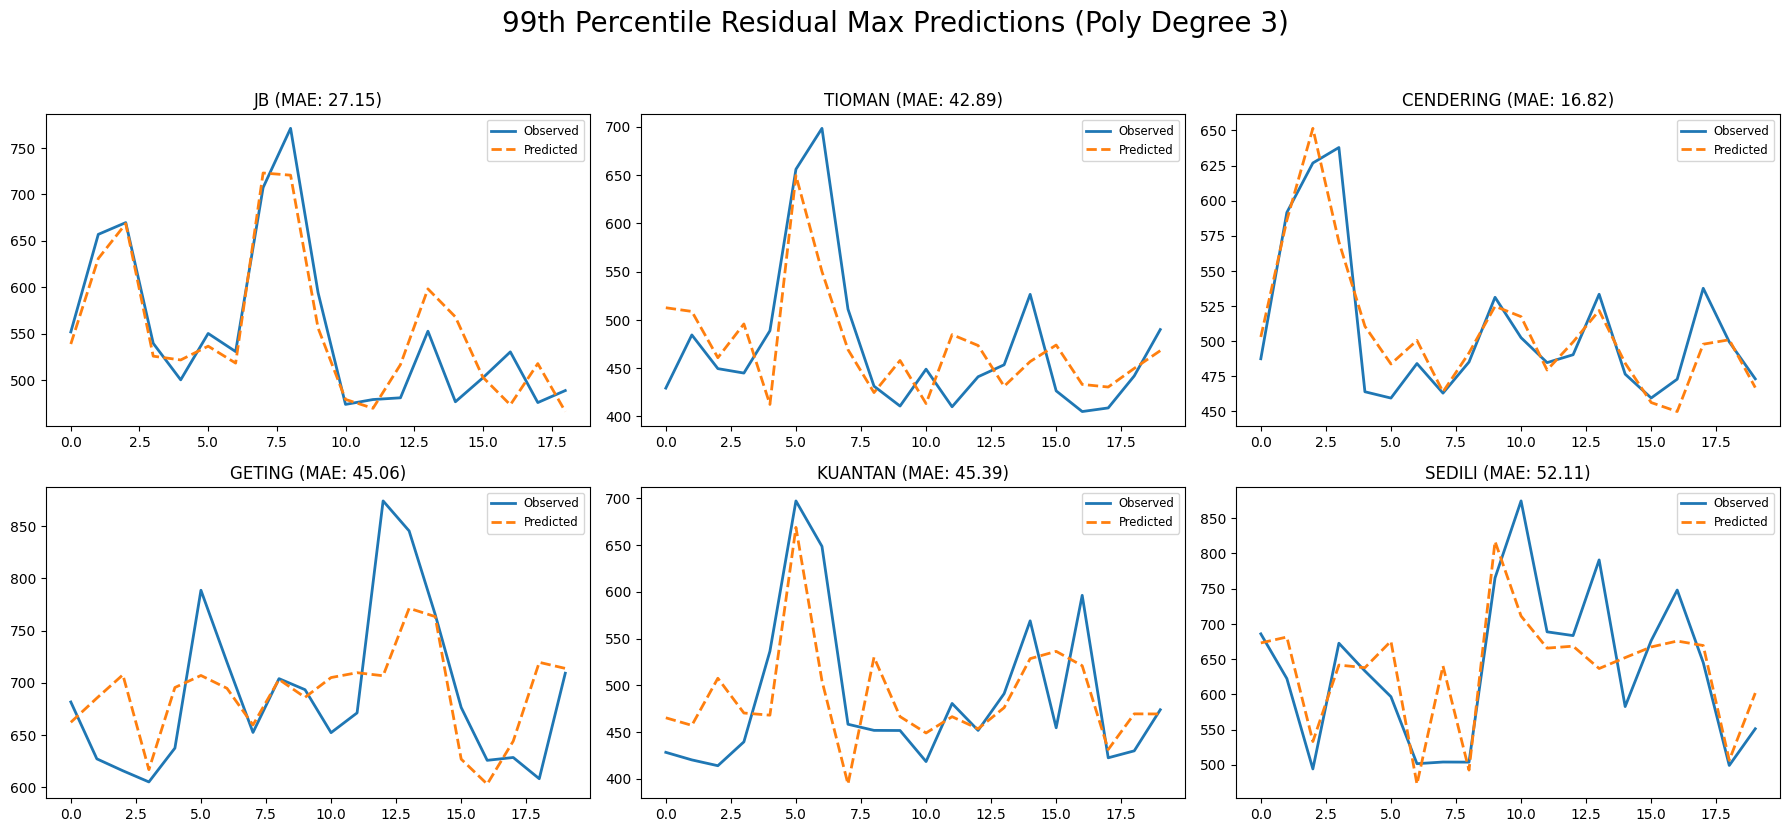
\includegraphics[width=\linewidth]{Figures/99th_percentile_all_locations.png}
        \caption{Comparison of predicted and observed values across Malaysian gauges using a cubic polynomial fit}
        \label{99_poly3_fit}
    \end{figure*}

  \begin{figure*}[htbp]
        \centering
        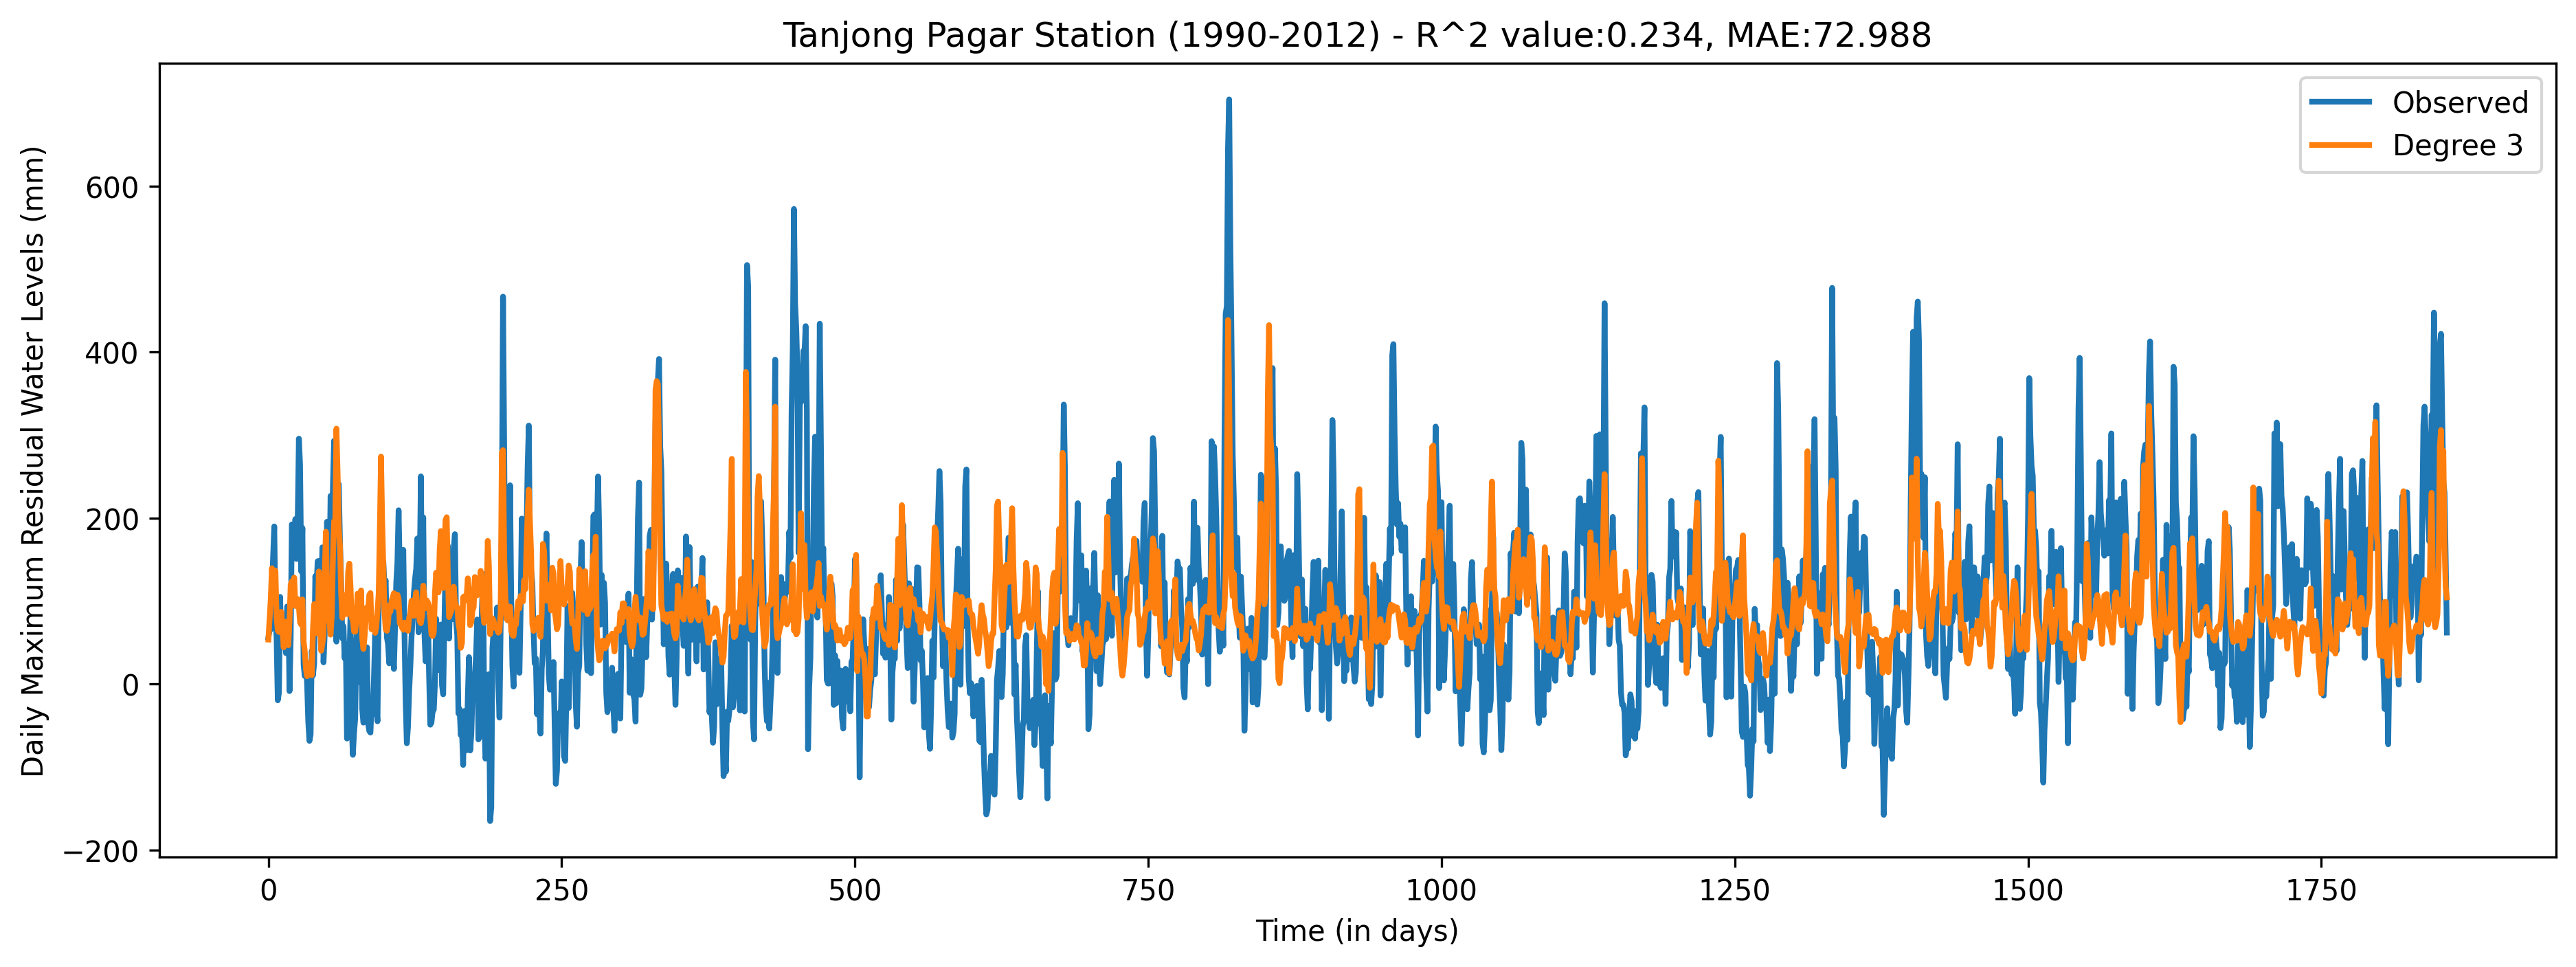
\includegraphics[width=\linewidth]{Figures/TP_Model_trained.png}
        \caption{Comparison of predicted and observed values for Tanjong Pagar station from 1990 to 2013 using a cubic polynomial fit}
        \label{tp_full_fit}
    \end{figure*} 

       \begin{paragraph}
        \noindent Figure \ref{tp_full_fit} compares the residual water levels predicted by the cubic polynomial model (in orange) compared with observed residual water levels from 1990 - 2012. The comparisons for the rest of the locations are provided in Appendix D. The R\textsuperscript{2} value of 0.234 and MAE of 72.988, illustrating the discrepancies between the model and the data around the most pronounced peaks. Table \ref{table_3} shows the coefficients for each component along with the intercept for the cubic polynomial fit across the seven gauges. From the table we can observe that Geting has the strongest correlation to both wind and MSLP. This is evident from the coefficients: for wind, Geting's first coefficient (2.2030e-03) is approximately 100 times larger than those of other locations (which are in the e-05 range). For MSLP, Geting's coefficient (3.3377e-03) is comparable to other locations, but when considered alongside the wind correlation, Geting stands out as having strong relationships with both variables. 
        \end{paragraph}
    

        \begin{paragraph}
            \noindent We've further cross-validated the model with other inputs from two distinct time periods: 1984-1986 (Figure \ref{hindcast_tp}) and 2014-2016 (Figure \ref{forecast_tp}) for Tanjong Pagar station. The corresponding figures for the remaining seven locations are provided in Appendix D. Throughout the validation periods, vertical red lines mark the days where cold surge events were observed. From an evaluation standpoint, these periods of peak water level activity, in combination with the cross-validation periods, are the most critical from a model performance standpoint and showcase the model’s ability to tackle extreme cases across diverse time periods. The validation demonstrates that while overall performance aligns with observed trends, there is a noticeable disparity where the highest surge events are underestimated.
        \end{paragraph}

        \begin{figure*}[htbp]
        \centering
        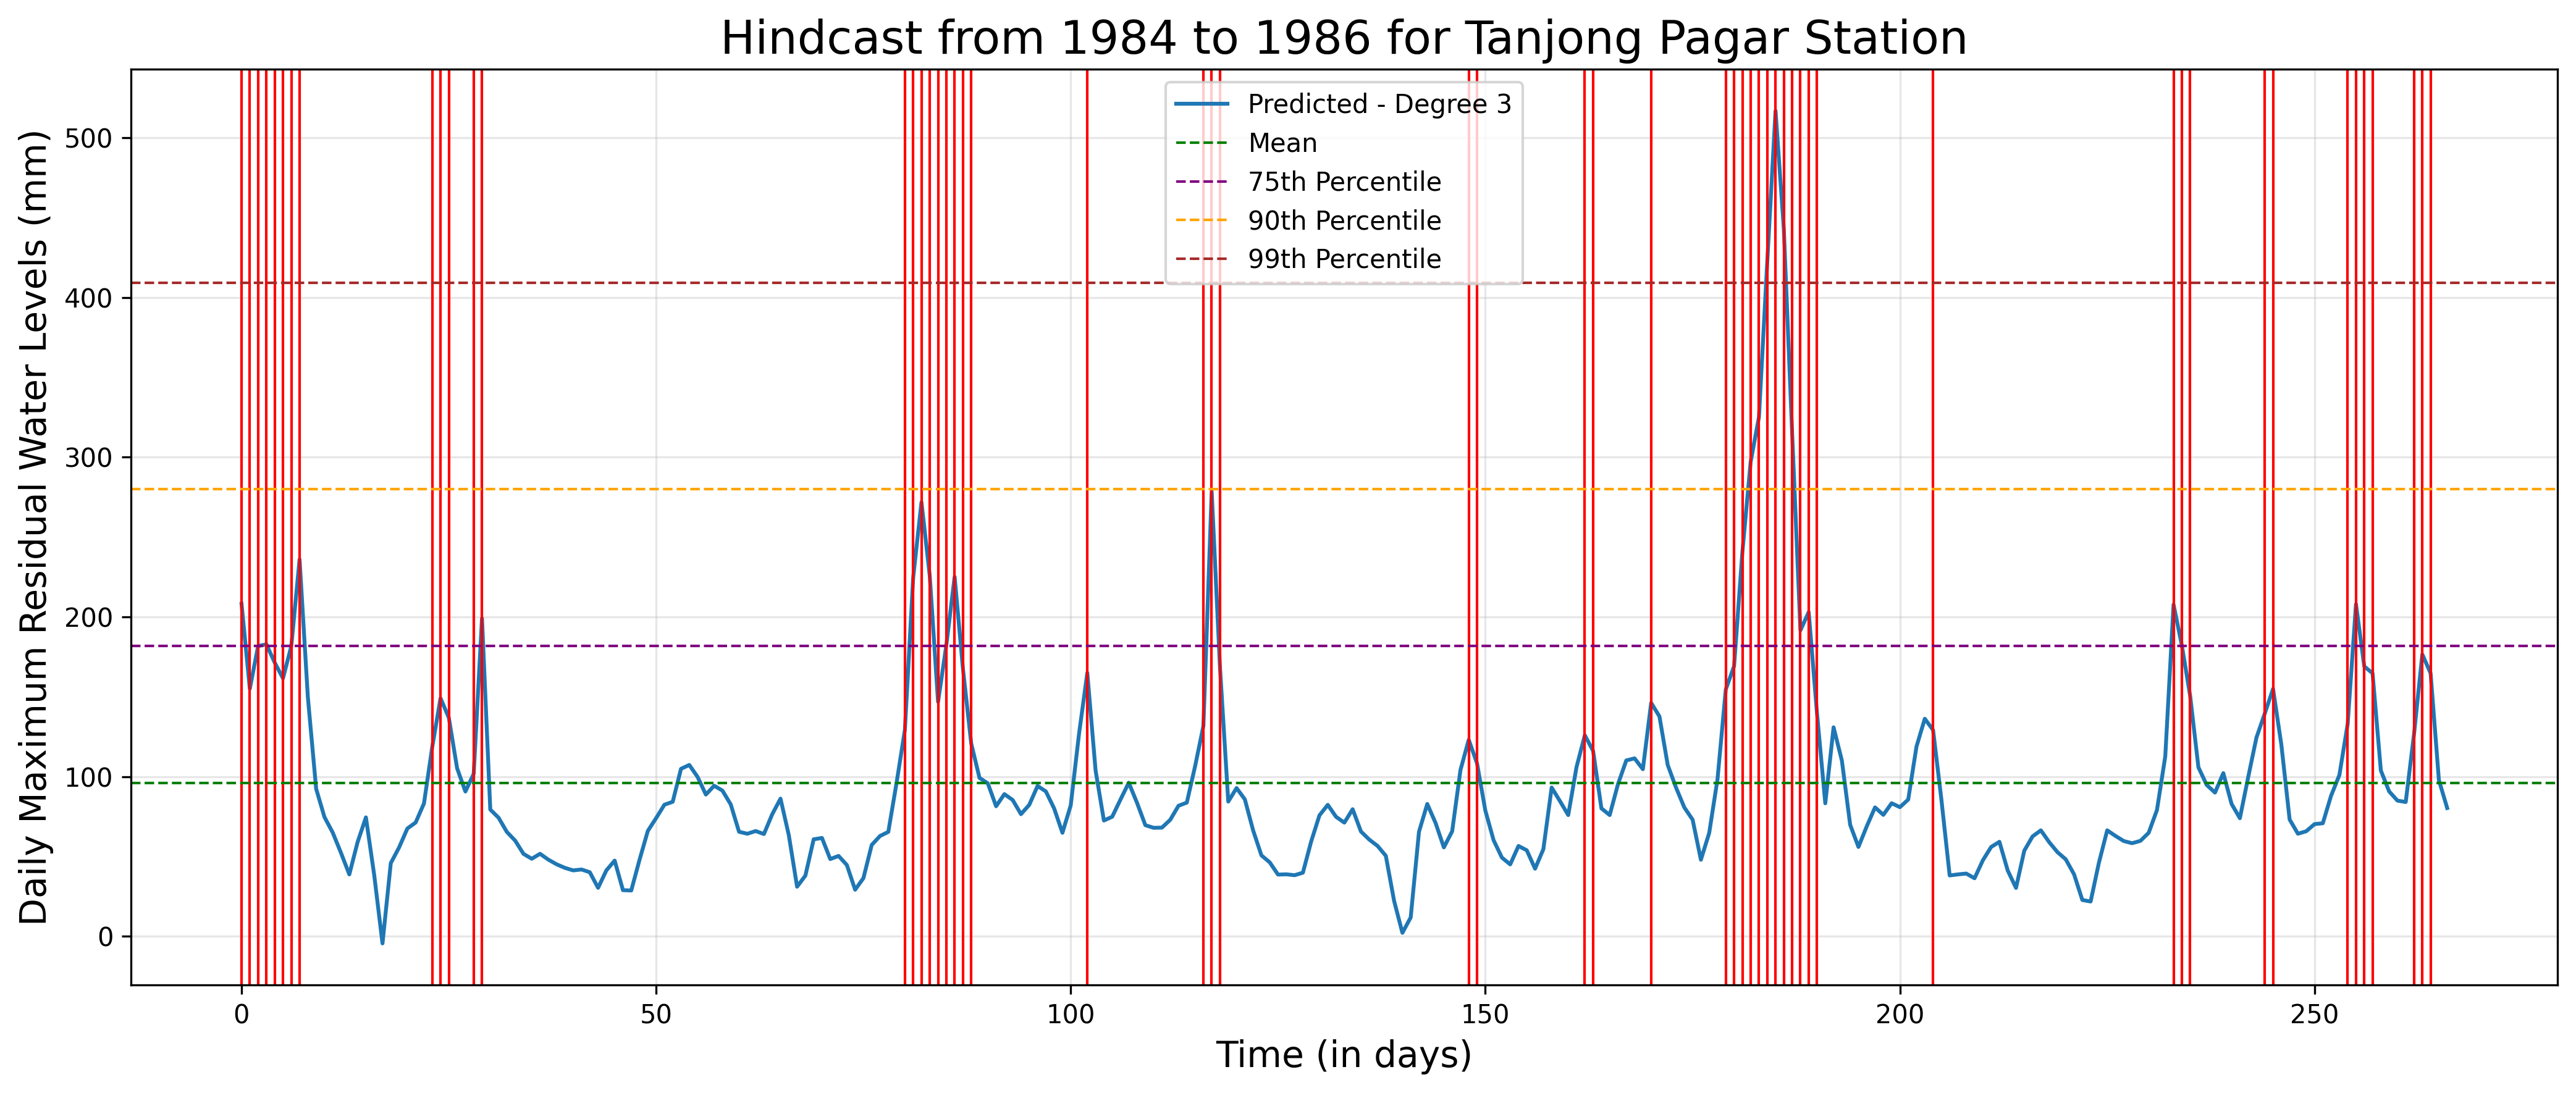
\includegraphics[width=\linewidth]{Figures/HIndcast_1984_1986_TP_SD.png}
        \caption{Behaviour of the model with respect to extreme sea levels and surge days from 1984-1986 at Tanjong Pagar Station}
        \label{hindcast_tp}
    \end{figure*}

    \begin{paragraph}
        \noindent Surge days for both the hindcast (1984-1986) and forecast (2014-2016) periods were accurately predicted, as shown by vertical red lines - the substantial peaks mostly coincide with the red vertical lines (which indicate a surge day). In both Figure 13 and 14, we can see that a reasonable estimate for the threshold for `extreme' tides lies around 75th percentile (purple dashed line) and 90th percentile (yellow dashed line). This optimal balance improves discrimination of actual surge events and minimizes false alarm detection. The model avoided using the 99th percentile which is too restrictive, while rising above 75th percentiles allows a balance between sensitivity and specificity. This allows us to strike a balance by reaching a practical compromise and making the prediction system reliable with further improvements.
    \end{paragraph}


    

    \begin{figure*}[htbp]
        \centering
        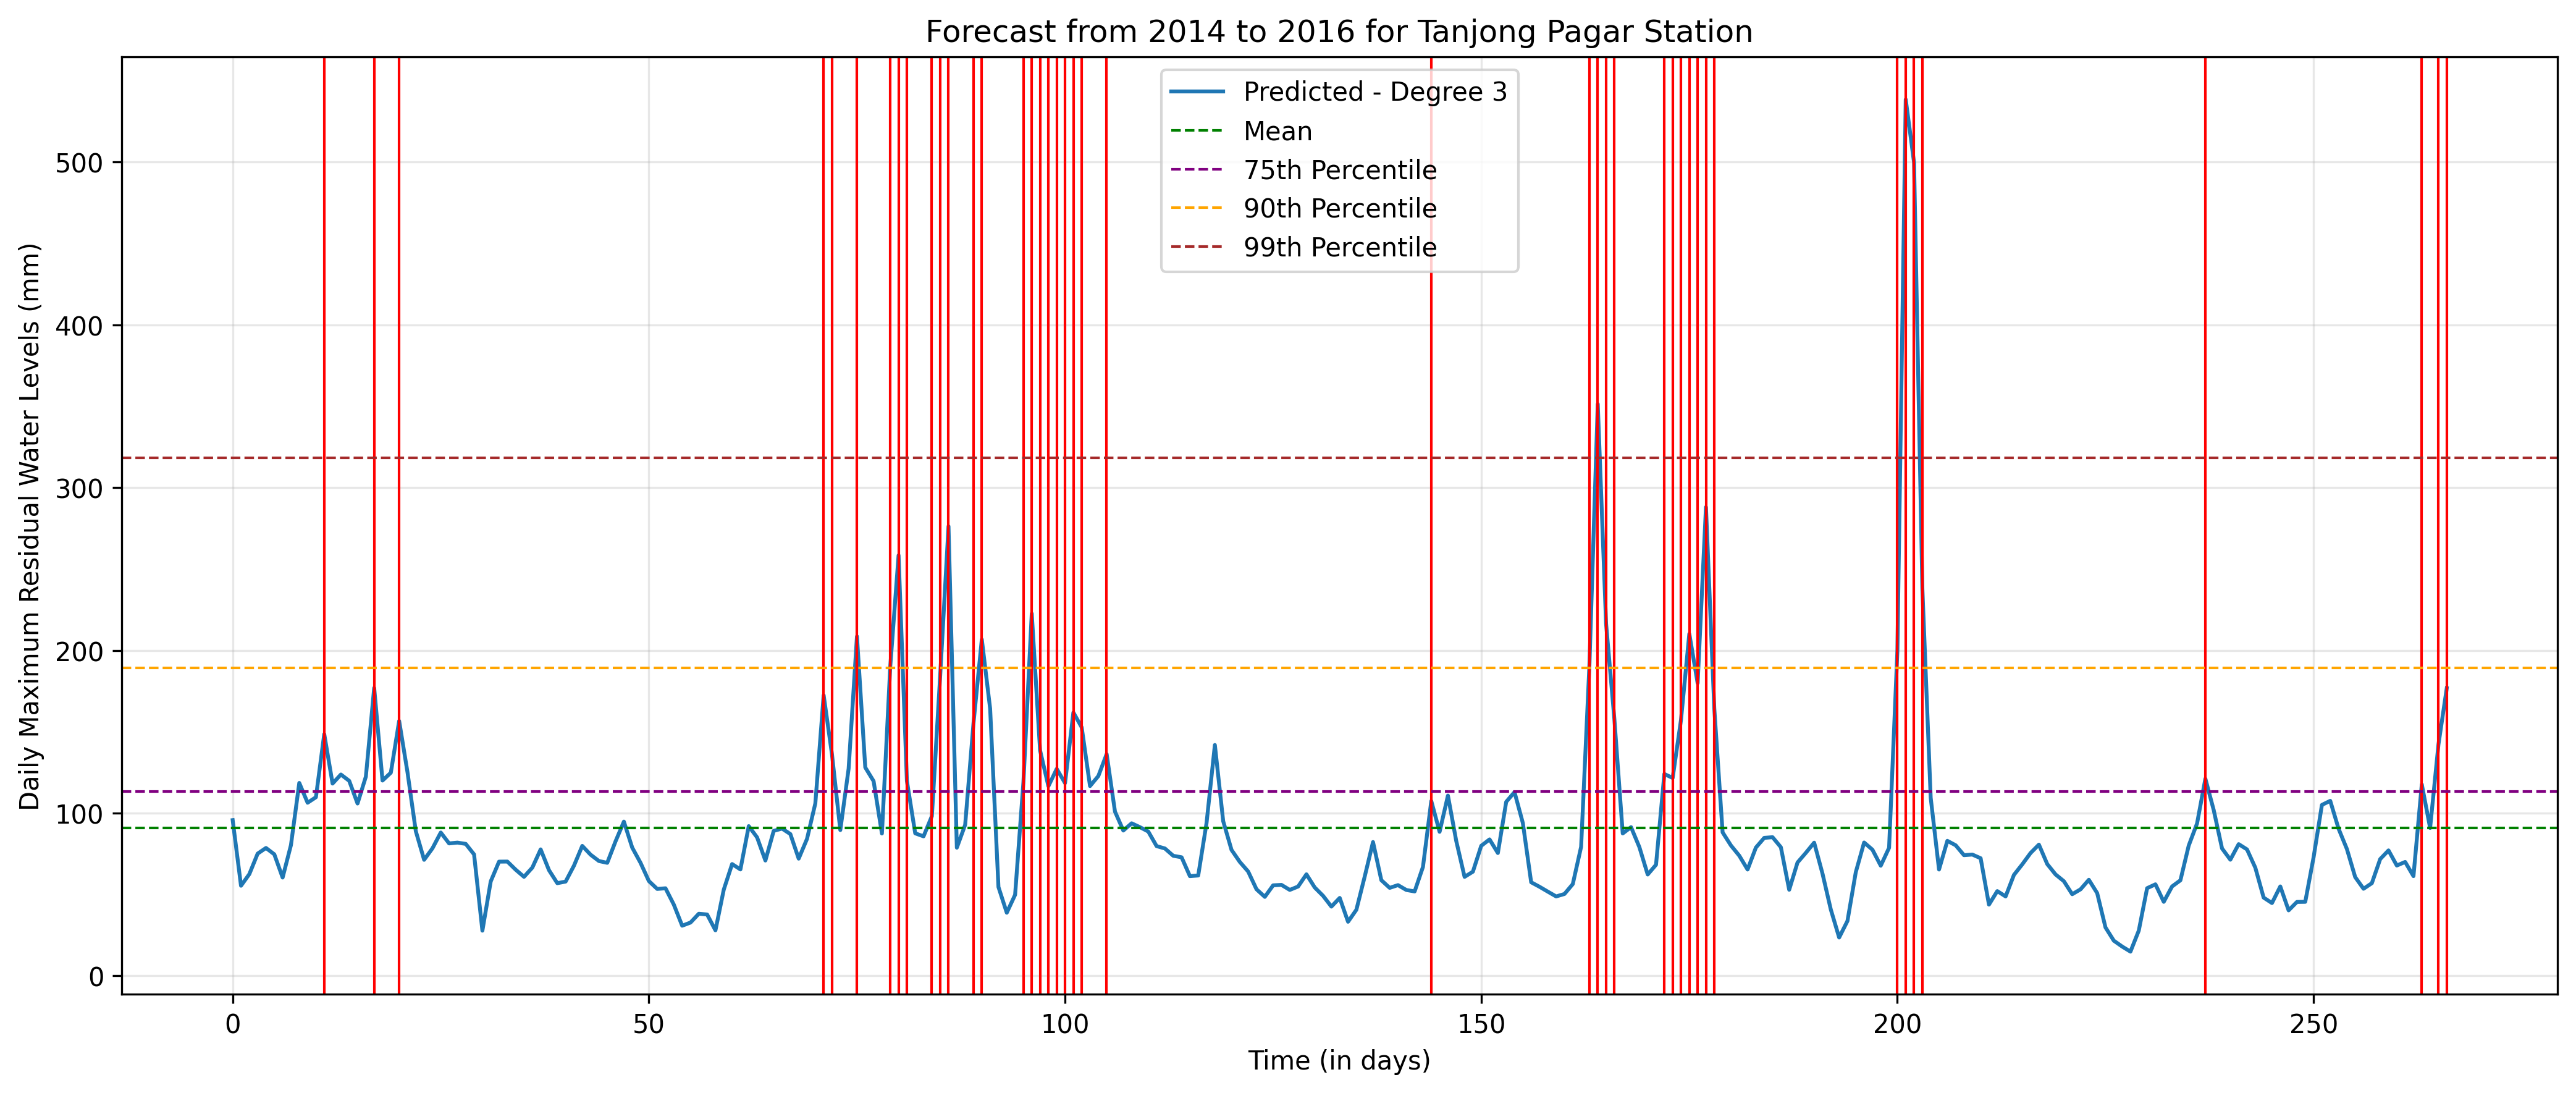
\includegraphics[width=\linewidth]{Figures/Forecast_2014_2016_TP_SD.png}
        \caption{Behaviour of the model with respect to extreme sea levels and surge days from 2014-2016 at Tanjong Pagar Station}
        \label{forecast_tp}
    \end{figure*}

    \newpage
    \section*{Limitations and Future Work}
    \addcontentsline{toc}{section}{Future Work}
    \begin{paragraph}
        \noindent The advancement of our climate model necessitates higher-resolution data gathering, that is, 6-minute frequencies rather than hourly observations. More temporal resolution would be better at identifying tidal behavior on downsampled analysis while maintaining the nuance of water level variability hourly observations cannot capture. This development demands access to more computational resources since the computation of the UTide harmonic analysis on such exponentially larger datasets exceeds our current resources. However we ensured that the methods used here are reproducible (with modifications to handling of the data structures) with a dataset of higher granularity as well.
    \end{paragraph}

    \begin{paragraph}
        \noindent To transcend traditional statistical methods, we recommend applying advanced deep learning methods such as Long Short-Term Memory (LSTM) networks and Deep Reinforcement Learning (DRL) models to forecast water level. These would potentially be able to spot more evasive, non-linear patterns of coastal water dynamics but would require using supercomputing centers. Second, our model framework must be expanded to encompass recognized climate oscillation indices, most importantly the El Niño-Southern Oscillation (ENSO) and Madden-Julian Oscillation (MJO) (\cite{Lim2017_MonsoonRainfall}), which have demonstrated significant influence on coastal water levels but as yet are not in our parameter set.
    \end{paragraph}

    \begin{paragraph}
        \noindent An overall appreciation of long-term `extreme' water level behavior requires our analysis time being lengthened to capture inter-decadal trends. Climate variability and long-term trends of increase in mean sea water level, operate on very large temporal scales that our current dataset cannot resolve fully. Access to longer records in the past would enable cyclical behavior and secular trends to be resolved. The longer dataset, along with the aforementioned increased granularity of data and model complexity, would dramatically enhance our forecasting ability for water levels under a changing climate.
    \end{paragraph}

    
   \section*{Conclusion}
    \addcontentsline{toc}{section}{Conclusion}
    \begin{paragraph}
        \noindent In this study, we aimed to mathematically explore the relation between residual water levels, with factors that lead to the development of cold surge events across a region of the Western Maritime Continent. We first established the difference between deterministic signals based on astronomical positions of the Sun and the Moon, and stochastic signals brought about by meteorological influences, using harmonic analysis. To predict daily maximum residual water levels, we tested several statistical frameworks incorporating wind speed and MSLP. The dependent variables were taken from two domains across the SCS, and cold surge indices were defined on the basis of these metrics, as per a relative methodolody that allows reproducibility across different locations.
    \end{paragraph}

    \begin{paragraph}
        \noindent  Among the tested models, including linear, quadratic, cubic polynomials, and L1/L2 regularized regressions, a cubic polynomial fit consistently demonstrated the best performance across all seven tide gauge locations, exhibiting the highest R\textsuperscript{2} values and the lowest mean absolute error. While the overall variance explained by the models was modest, the cubic model captured non-linear relationships in the data more effectively than simpler or regularized approaches. Cross-validation of the cubic polynomial model on independent time periods (1984-1986 and 2014-2016) revealed its ability to generally align with observed water level trends and accurately identify surge days. Analysis of the model's performance during these periods suggested that a threshold between the 75th and 90th percentile offered a balanced approach for defining 'extreme' tides in the context of CS events.
    \end{paragraph}

    \begin{paragraph}
        \noindent Our study acknowledges limitations, including the hourly resolution of the available water level data and the exclusion of other significant climate oscillation indices. Future work should focus on incorporating higher-resolution data (such as the data obtained from the MPA), integrating influences from phenomena like ENSO and MJO, and employing statistical and machine learning frameworks to enhance predictive capabilities. Furthermore, extending the analysis to longer historical datasets will be crucial for capturing inter-decadal trends and improving our understanding of surge-induced flooding risks in a changing climate, ultimately aiding disaster preparedness and risk mitigation strategies in Southeast Asia.
    \end{paragraph}
    
     % <- This now properly ends the 2-column layout
\end{multicols}

\newpage
\bibliographystyle{agsm} % Choose your bibliography style
\bibliography{references}

\newpage
\section*{Appendices}
\addcontentsline{toc}{section}{Appendices}
\addcontentsline{toc}{subsection}{Appendix A - Distribution of datasets}
\subsection*{Appendix A - Distribution of datasets}
\begin{itemize}
    \item Distribution of Wind Speeds
    \begin{figure*}[htbp]
        \centering
        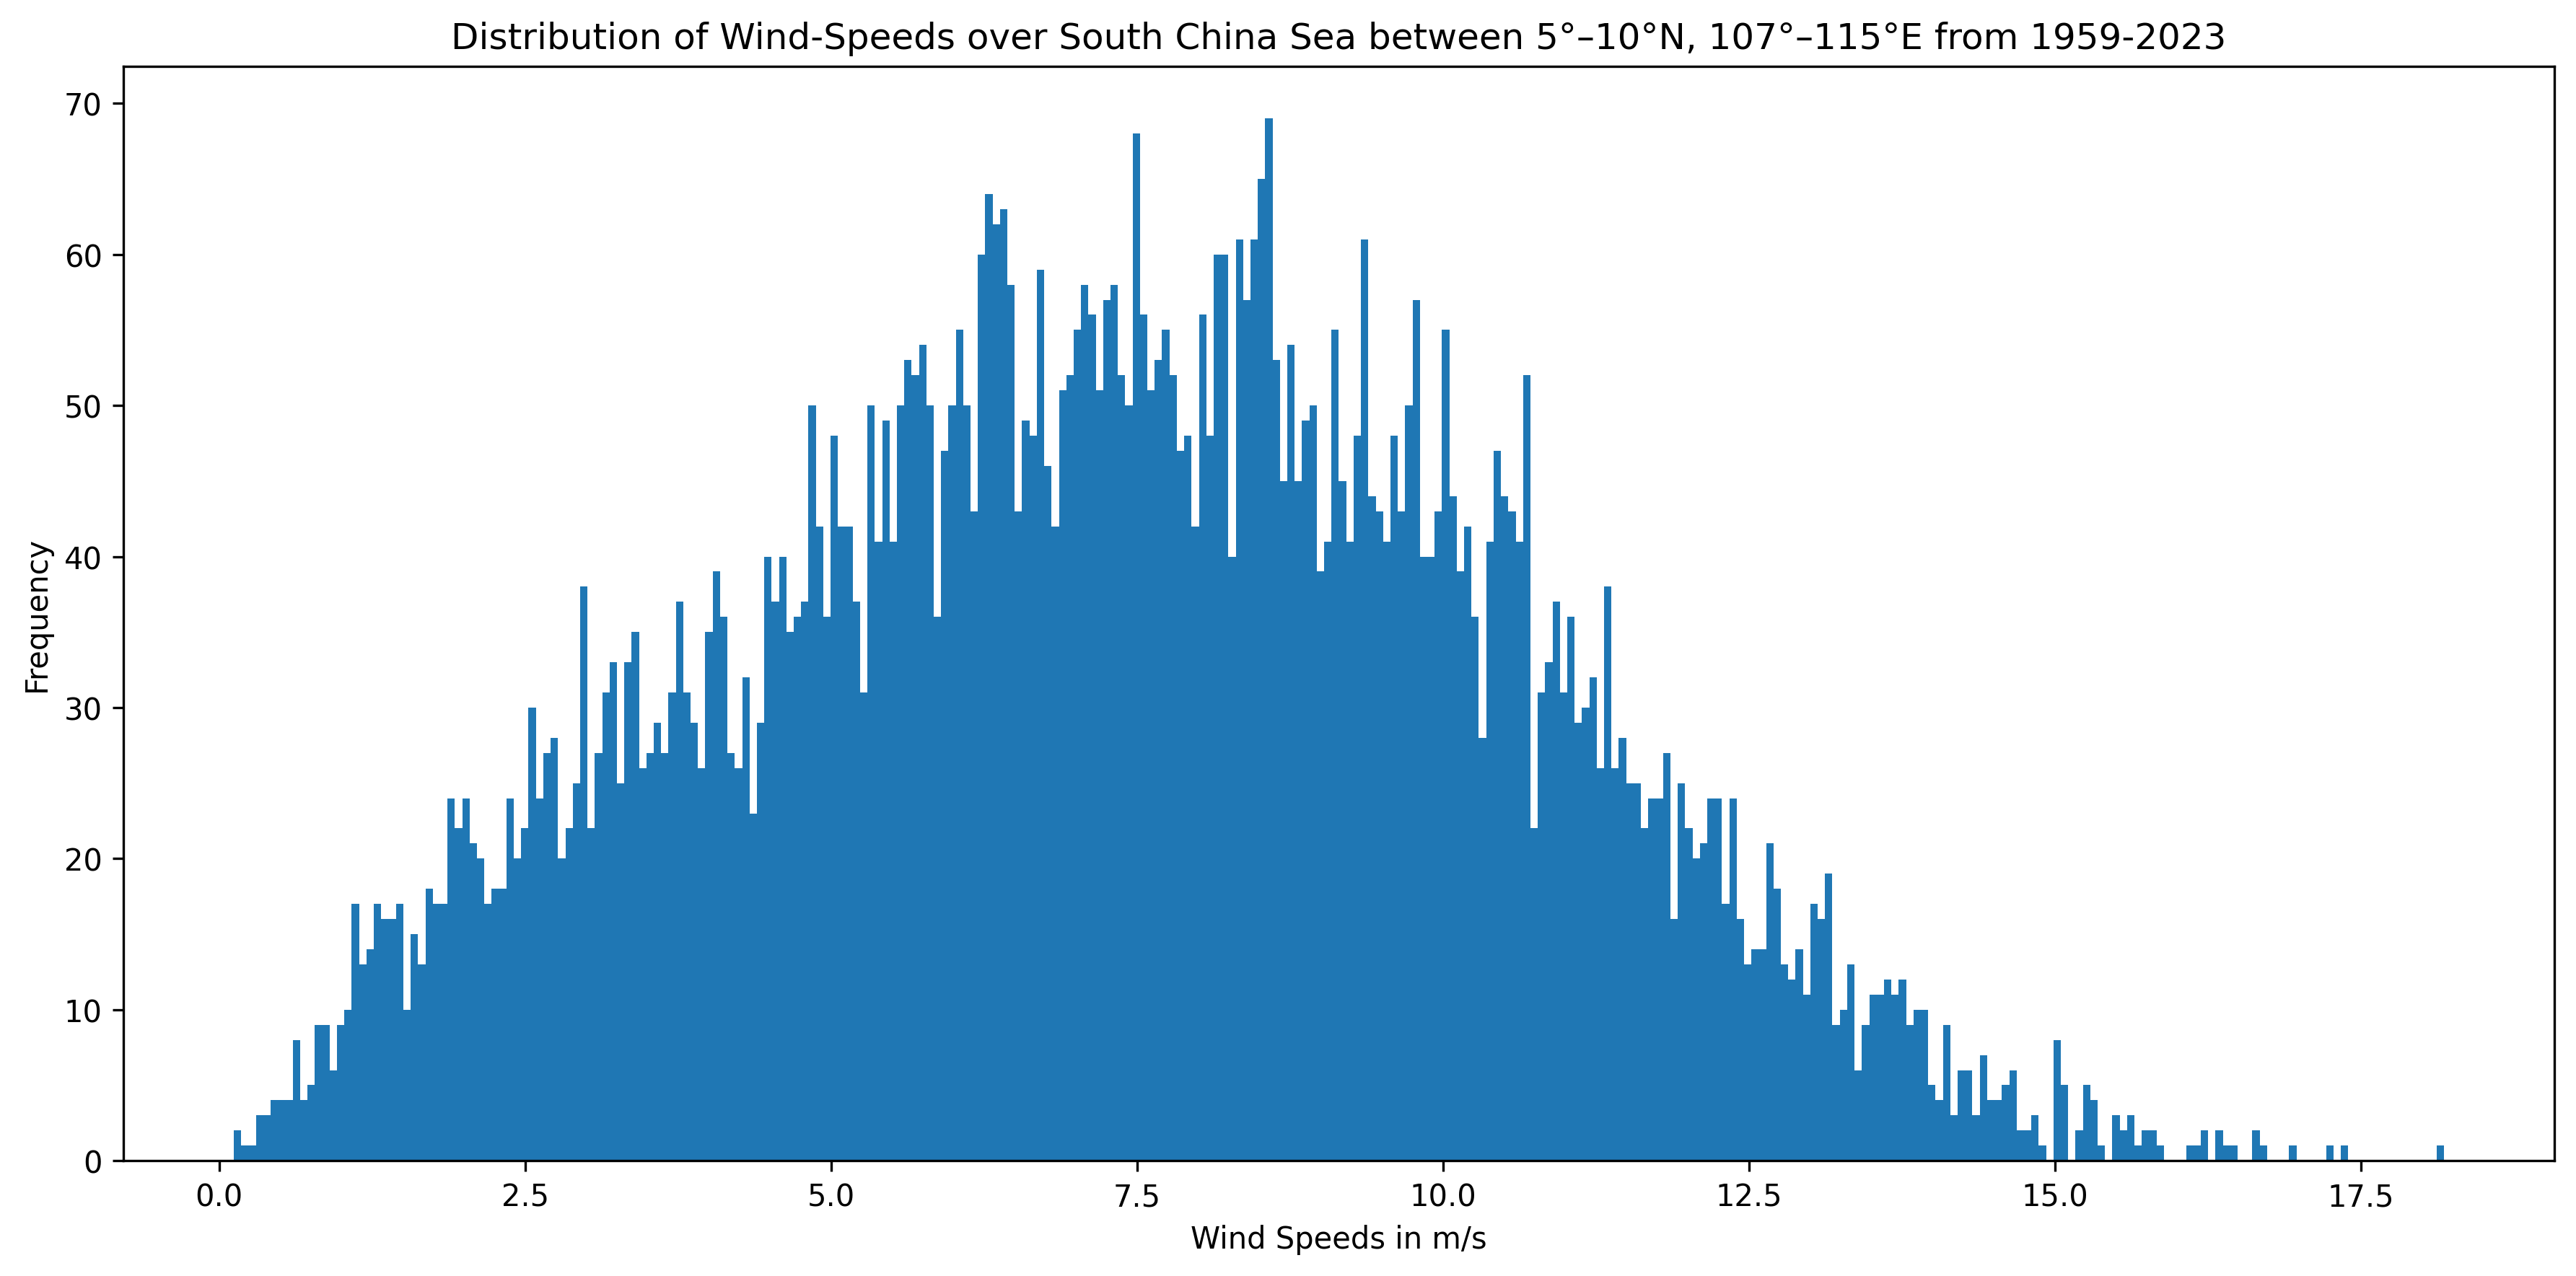
\includegraphics[width=0.8\linewidth]{Figures/Wind_Speed_Dist_1959_2023.png}
        \caption{Distribution of Area-Weighted Average of Wind Speeds over D1 from 1959 - 2023}
        \label{fig:enter-label}
    \end{figure*}
    \item Distribution of Mean Sea Level Pressure
    \begin{figure*}[htbp]
        \centering
        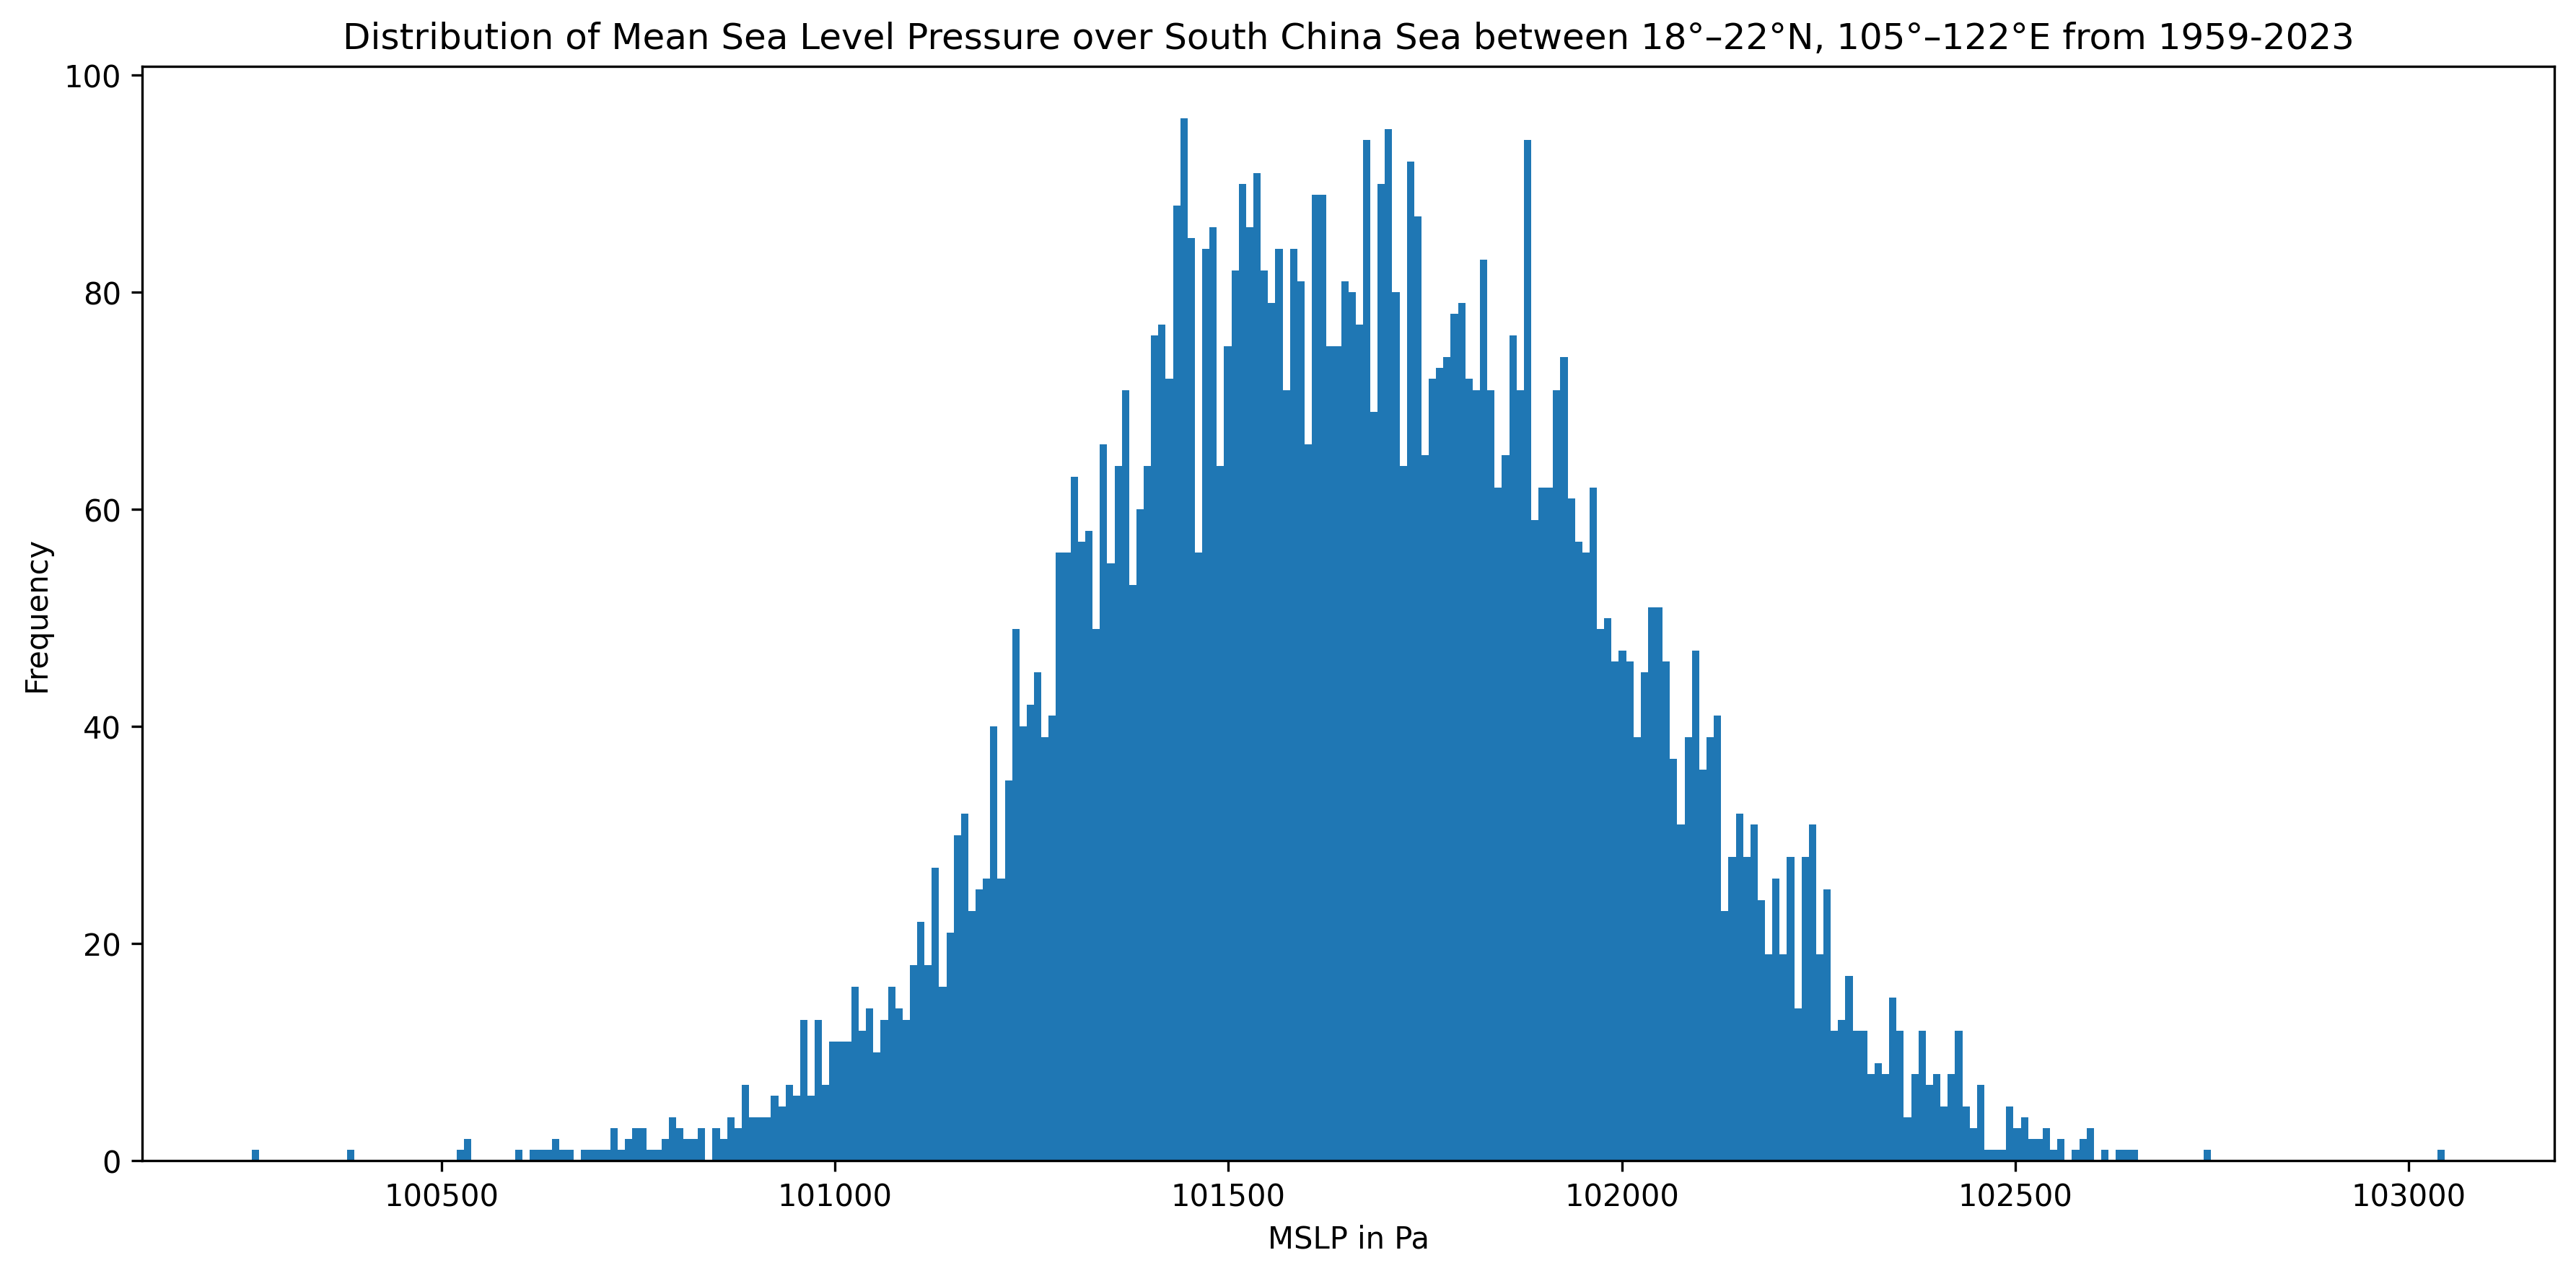
\includegraphics[width=0.8\linewidth]{Figures/MSLP_Dist_1959_2023.png}
        \caption{Distribution of Area-Weighted Average of MSLP over D2 from 1959 - 2023}
        \label{fig:enter-label}
    \end{figure*}
\end{itemize}
\newpage
\subsection*{Appendix B - UTide Results}
\addcontentsline{toc}{subsection}{Appendix B - UTide Results}
\begin{itemize}
    \item Cendering :
    \begin{itemize}
        \item Total Water Level
        \begin{figure*}[htbp]
        \centering
        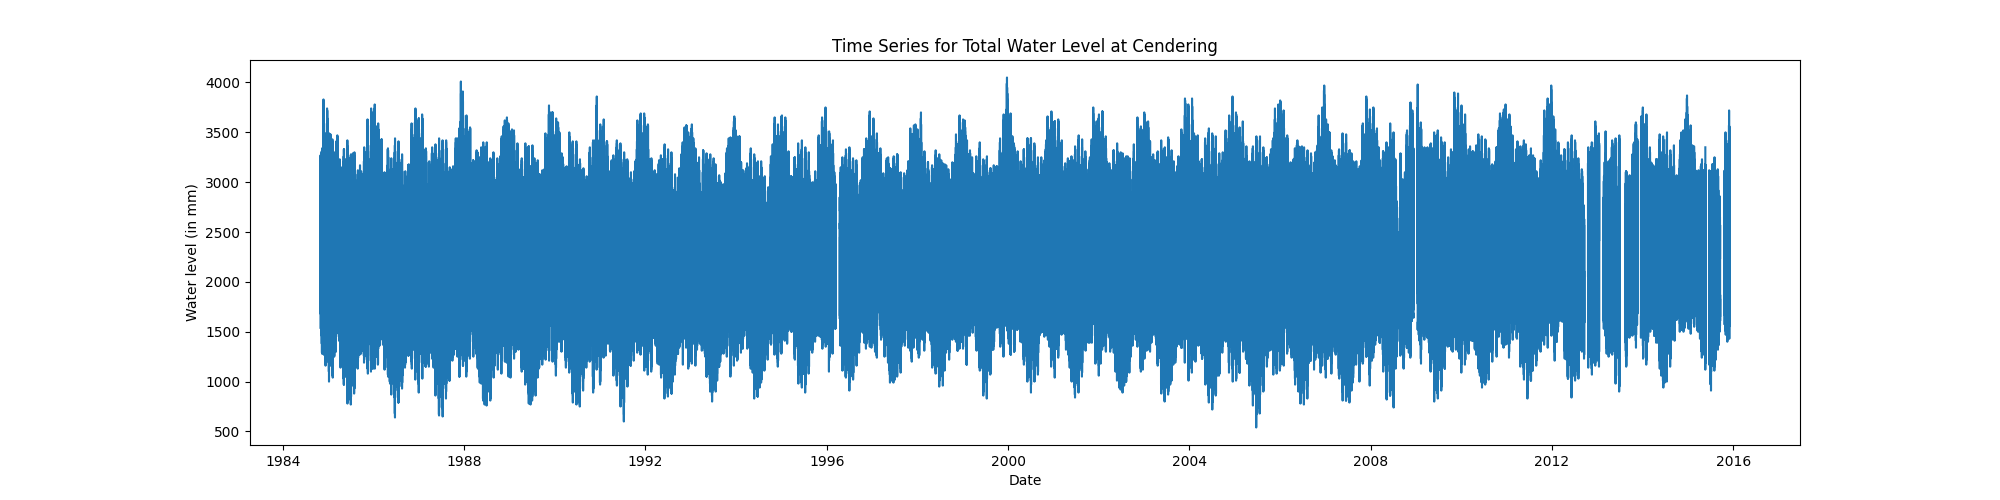
\includegraphics[width=\linewidth]{Figures/Time Series for Total Water Level at Cendering.png}
        \caption{Total Water Level at Cendering}
    \end{figure*}
    \item Predicted Water Level
        \begin{figure*}[htbp]
        \centering
        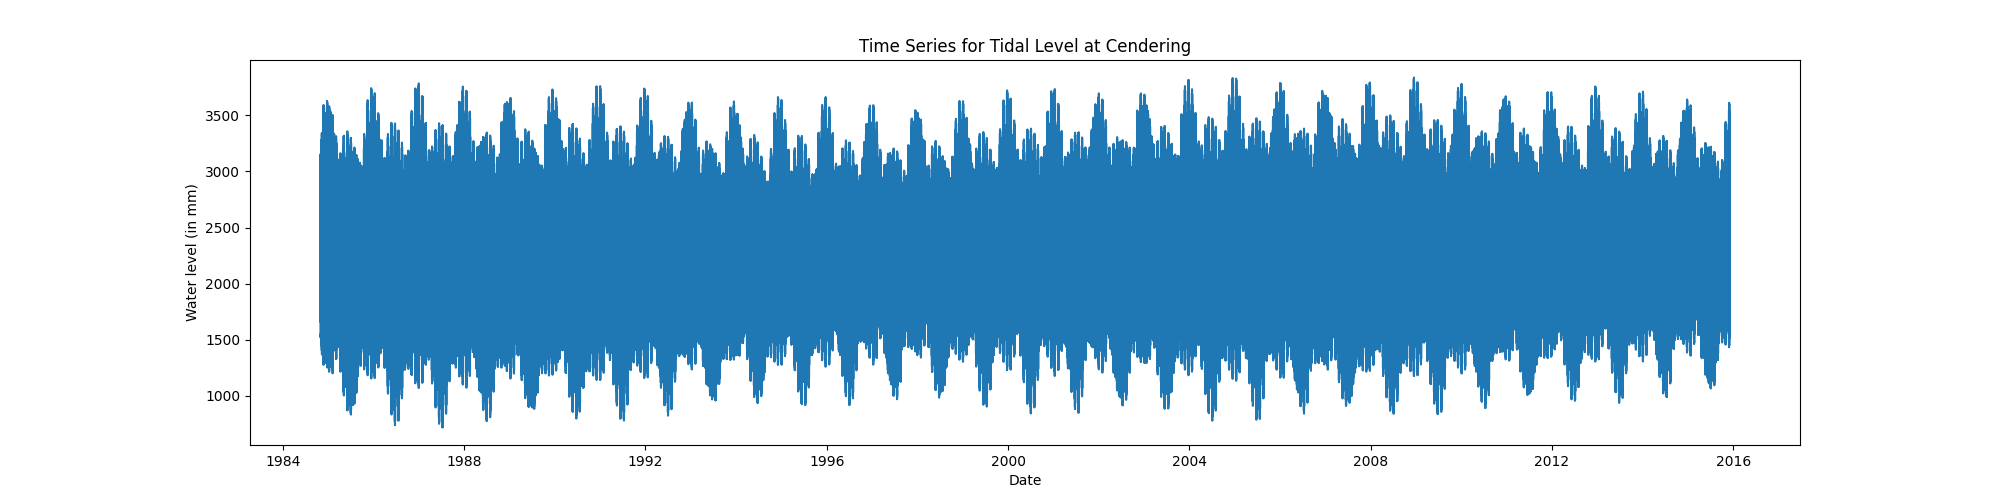
\includegraphics[width=\linewidth]{Figures/Time Series for Tidal Level at Cendering.png}
        \caption{Predicted Water Level at Cendering}
    \end{figure*}
    \item Residual Water Level
        \begin{figure*}[htbp]
        \centering
        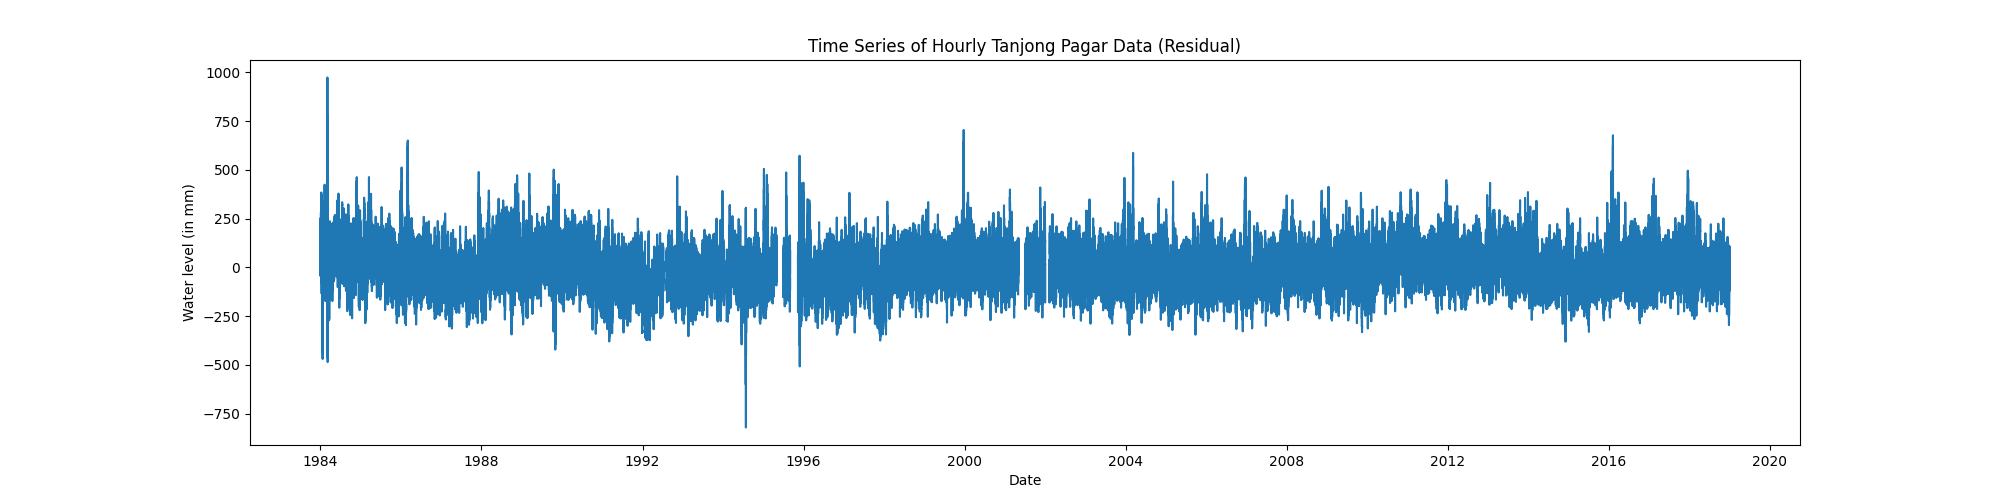
\includegraphics[width=\linewidth]{Figures/Time Series of Hourly Tanjong Pagar Data (Residual).png}
        \caption{Residual Water Level at Cendering}
    \end{figure*}
    \end{itemize}
\newpage
    \item Geting :
    \begin{itemize}
        \item Total Water Level
        \begin{figure*}[htbp]
        \centering
        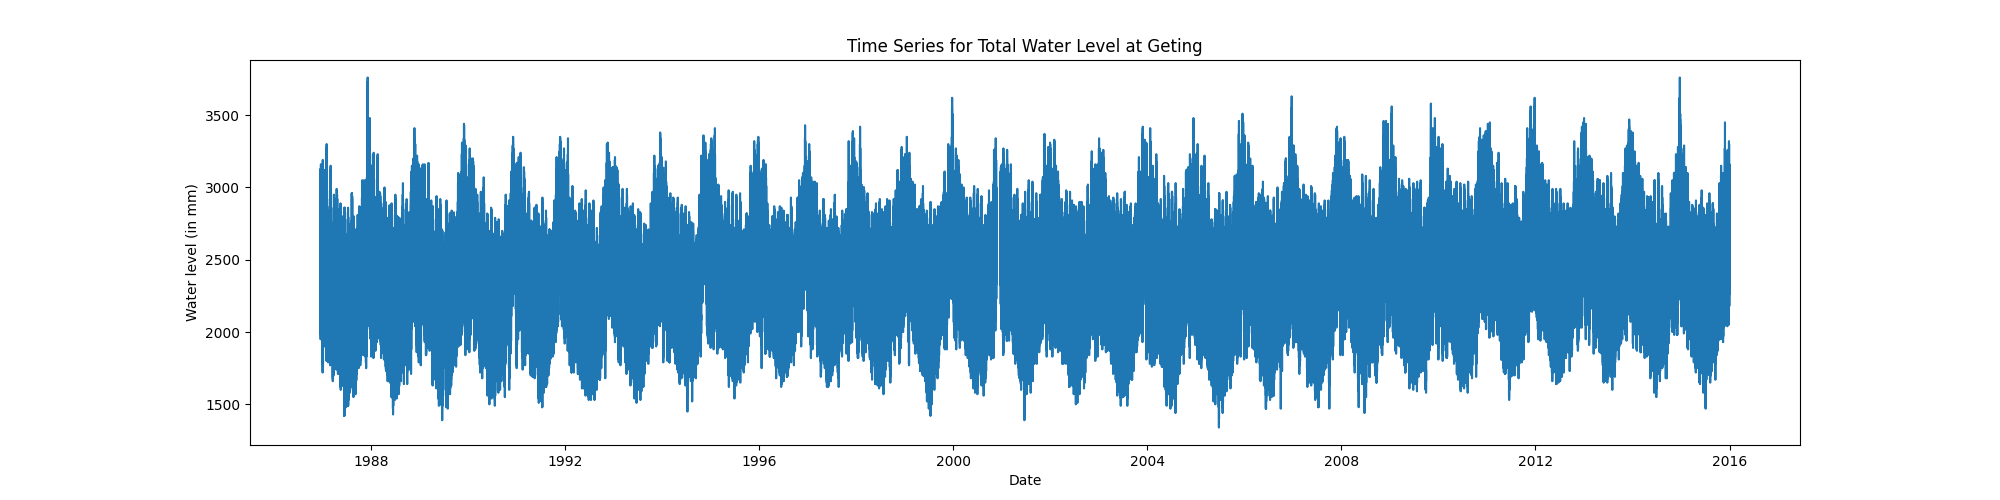
\includegraphics[width=\linewidth]{Figures/Time Series for Total Water Level at Geting.png}
        \caption{Total Water Level at Geting}
    \end{figure*}
    \item Predicted Water Level
        \begin{figure*}[htbp]
        \centering
        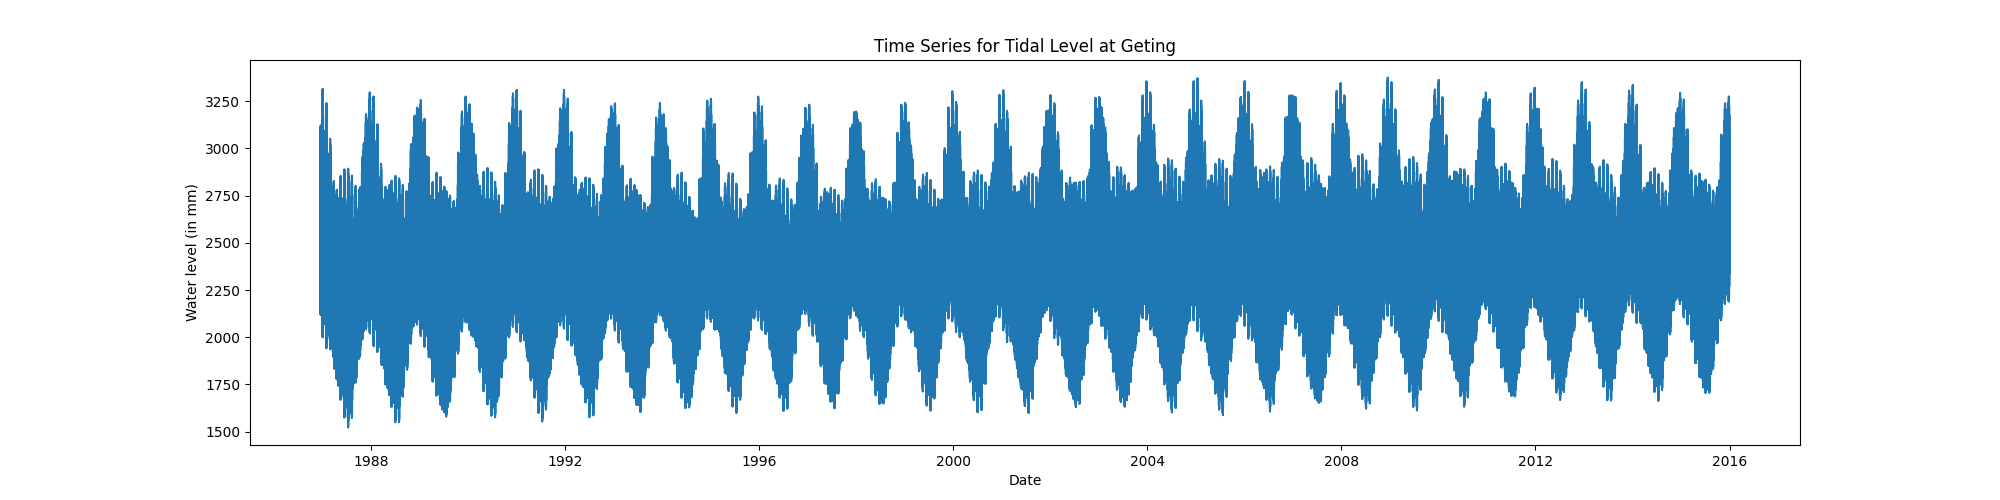
\includegraphics[width=\linewidth]{Figures/Time Series for Tidal Level at Geting.png}
        \caption{Predicted Water Level at Geting}
    \end{figure*}
    \item Residual Water Level
        \begin{figure*}[htbp]
        \centering
        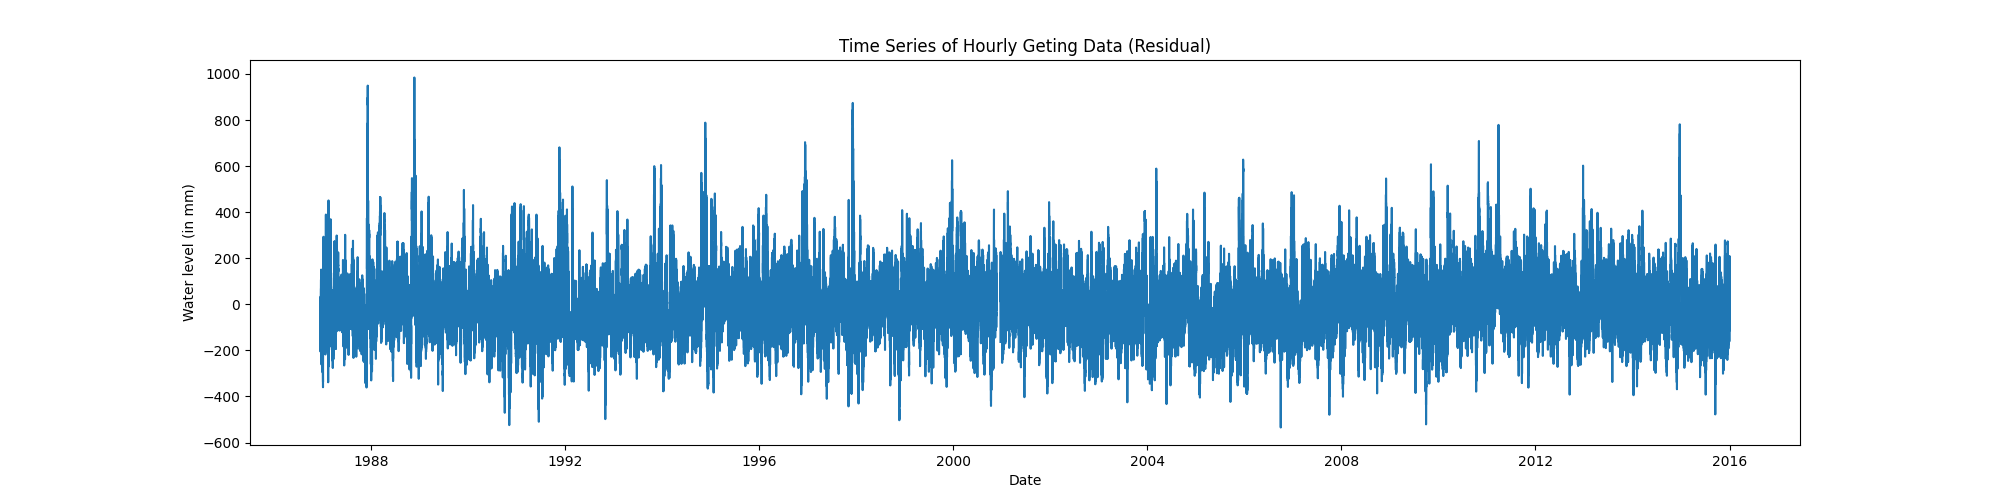
\includegraphics[width=\linewidth]{Figures/Time Series of Hourly Geting Data (Residual).png}
        \caption{Residual Water Level at Geting}
    \end{figure*}
    \end{itemize}
\newpage
        \item Kuantan :
    \begin{itemize}
        \item Total Water Level
        \begin{figure*}[htbp]
        \centering
        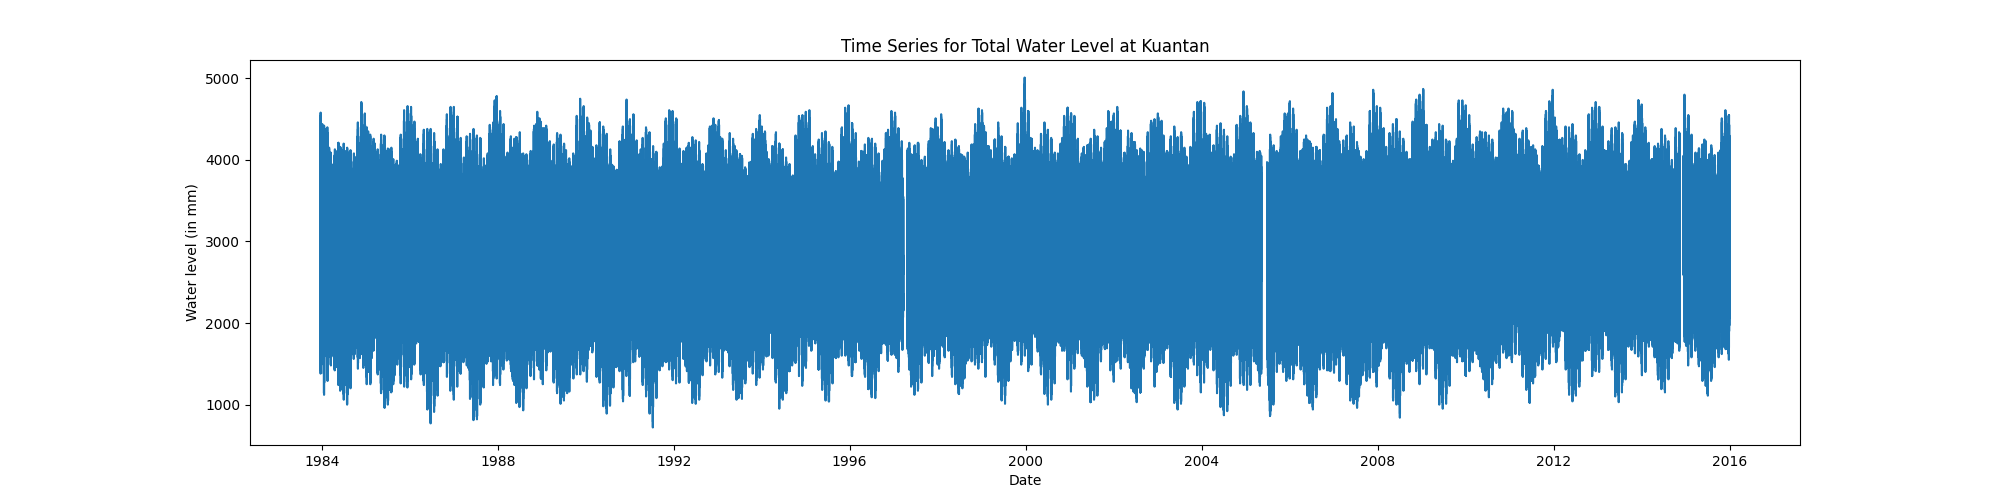
\includegraphics[width=\linewidth]{Figures/Time Series for Total Water Level at Kuantan.png}
        \caption{Total Water Level at Kuantan}
    \end{figure*}
    \item Predicted Water Level
        \begin{figure*}[htbp]
        \centering
        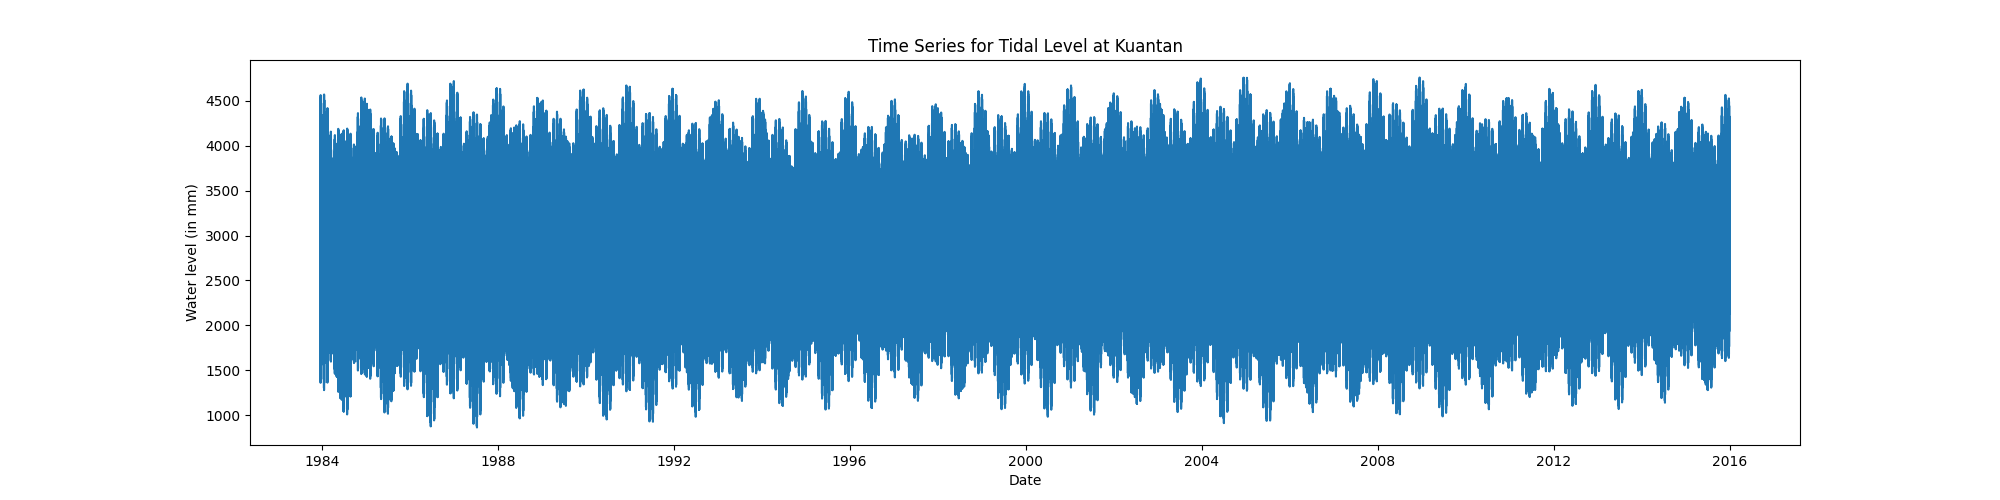
\includegraphics[width=\linewidth]{Figures/Time Series for Tidal Level at Kuantan.png}
        \caption{Predicted Water Level at Kuantan}
    \end{figure*}
    \item Residual Water Level
        \begin{figure*}[htbp]
        \centering
        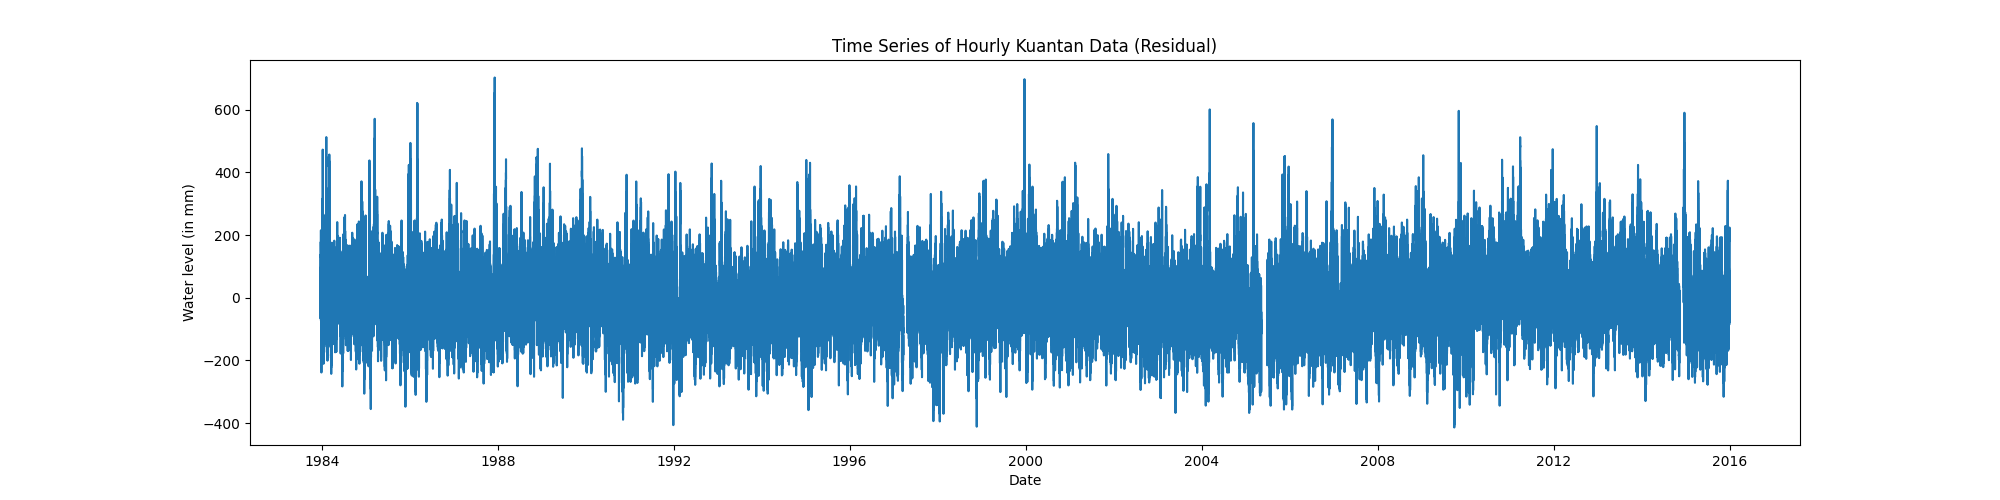
\includegraphics[width=\linewidth]{Figures/Time Series of Hourly Kuantan Data (Residual).png}
        \caption{Residual Water Level at Kuantan}
    \end{figure*}
    \end{itemize}
\newpage
        \item Johor Baharu :
    \begin{itemize}
        \item Total Water Level
        \begin{figure*}[htbp]
        \centering
        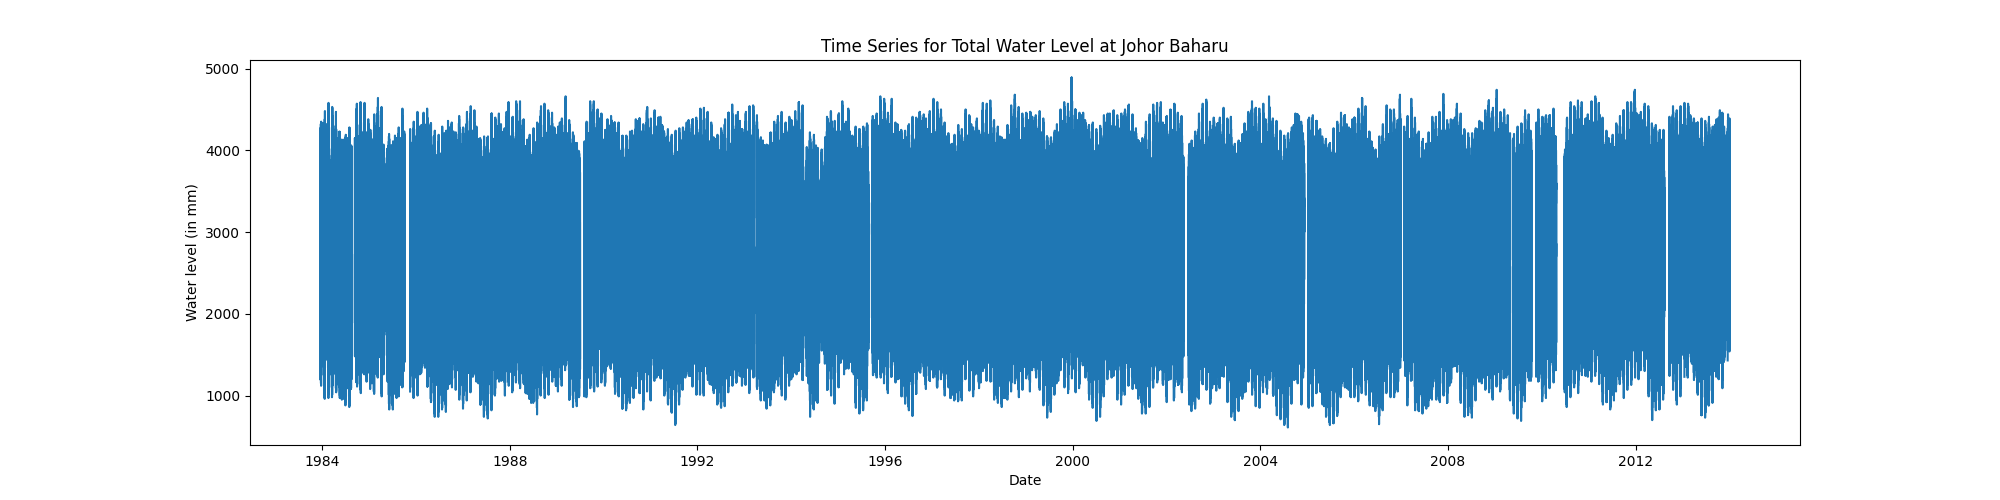
\includegraphics[width=\linewidth]{Figures/Time Series for Total Water Level at Johor Baharu.png}
        \caption{Total Water Level at Johor Baharu}
    \end{figure*}
    \item Predicted Water Level
        \begin{figure*}[htbp]
        \centering
        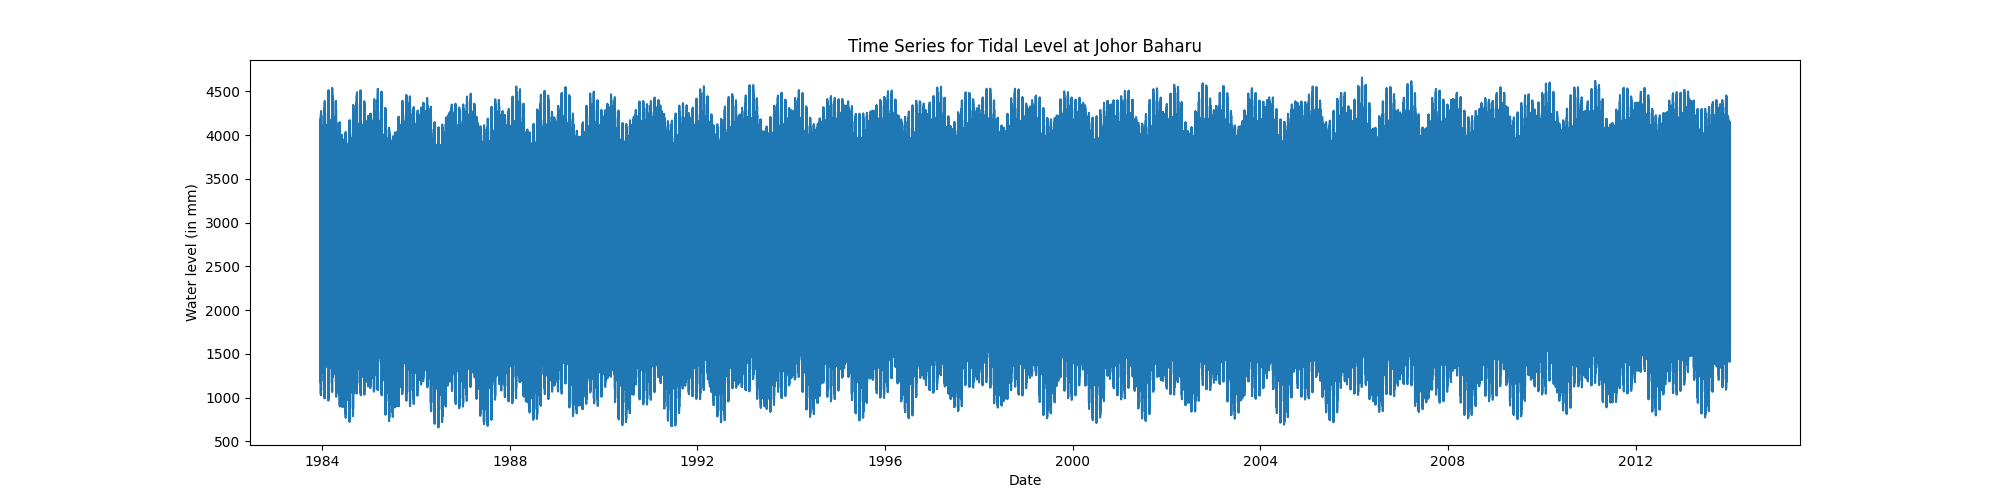
\includegraphics[width=\linewidth]{Figures/Time Series for Tidal Level at Johor Baharu.png}
        \caption{Predicted Water Level at Johor Baharu}
    \end{figure*}
    \item Residual Water Level
        \begin{figure*}[htbp]
        \centering
        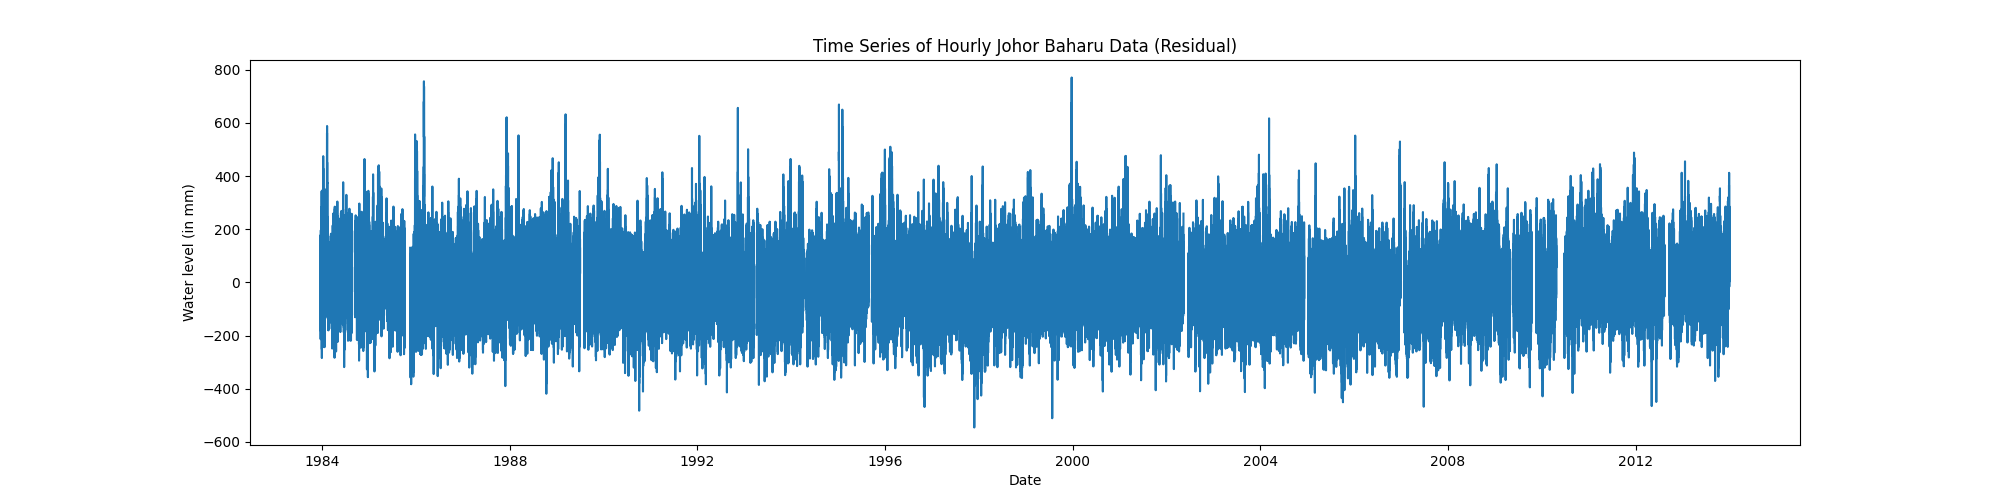
\includegraphics[width=\linewidth]{Figures/Time Series of Hourly Johor Baharu Data (Residual).png}
        \caption{Residual Water Level at Johor Baharu}
    \end{figure*}
    \end{itemize}
\newpage
        \item Sedili :
    \begin{itemize}
        \item Total Water Level
        \begin{figure*}[htbp]
        \centering
        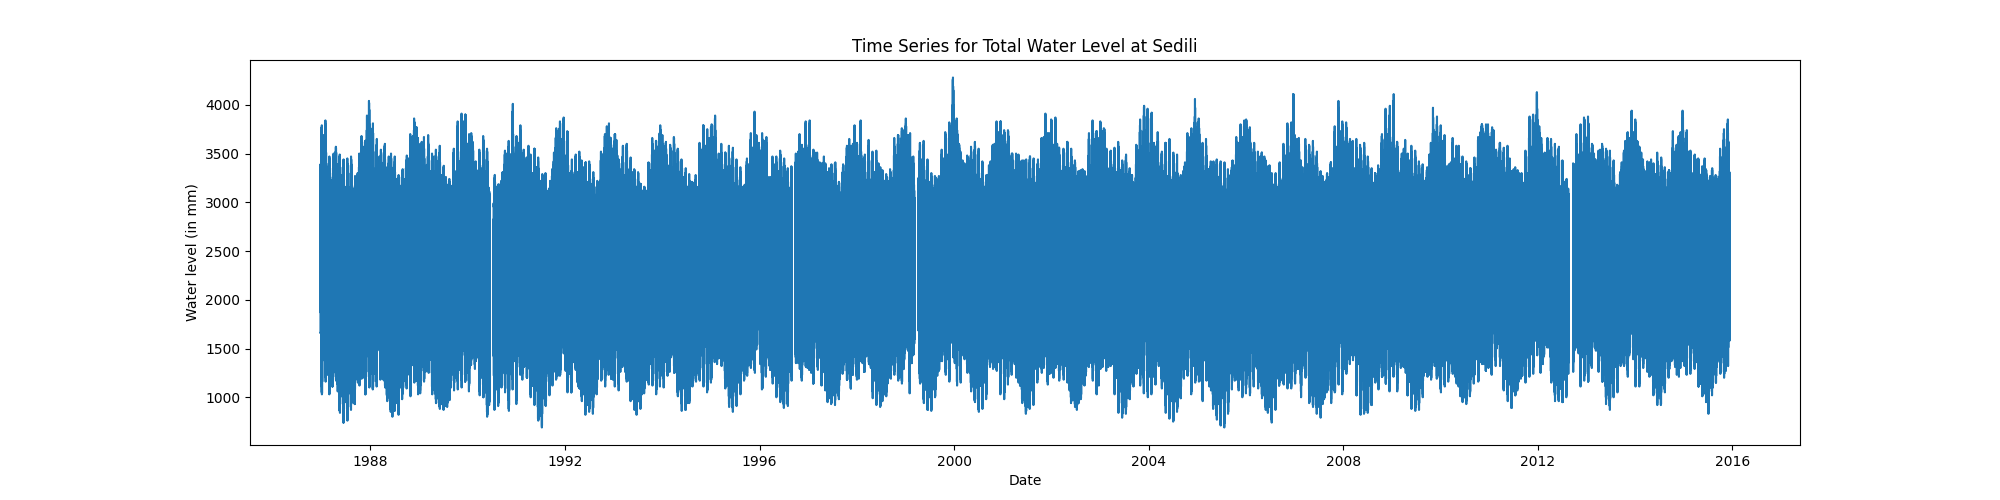
\includegraphics[width=\linewidth]{Figures/Time Series for Total Water Level at Sedili.png}
        \caption{Total Water Level at Sedili}
    \end{figure*}
    \item Predicted Water Level
        \begin{figure*}[htbp]
        \centering
        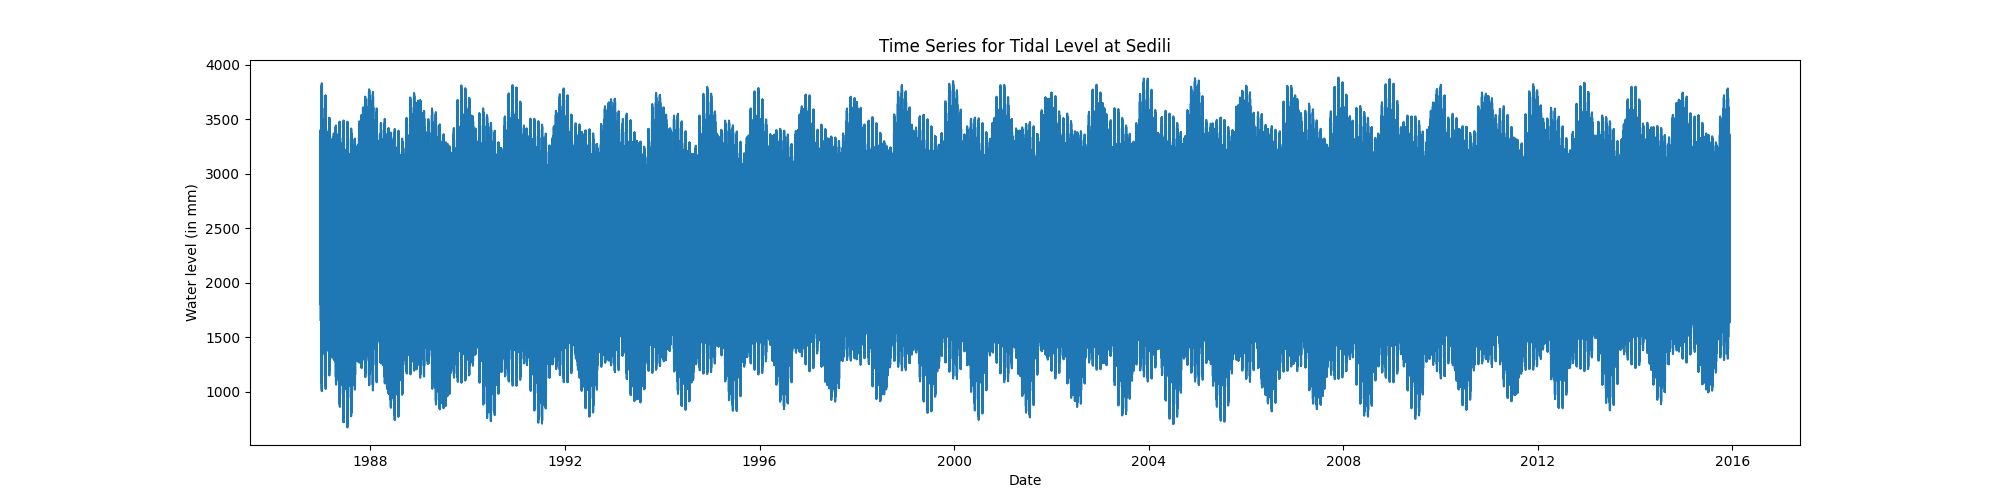
\includegraphics[width=\linewidth]{Figures/Time Series for Tidal Level at Sedili.png}
        \caption{Predicted Water Level at Sedili}
    \end{figure*}
    \item Residual Water Level
        \begin{figure*}[htbp]
        \centering
        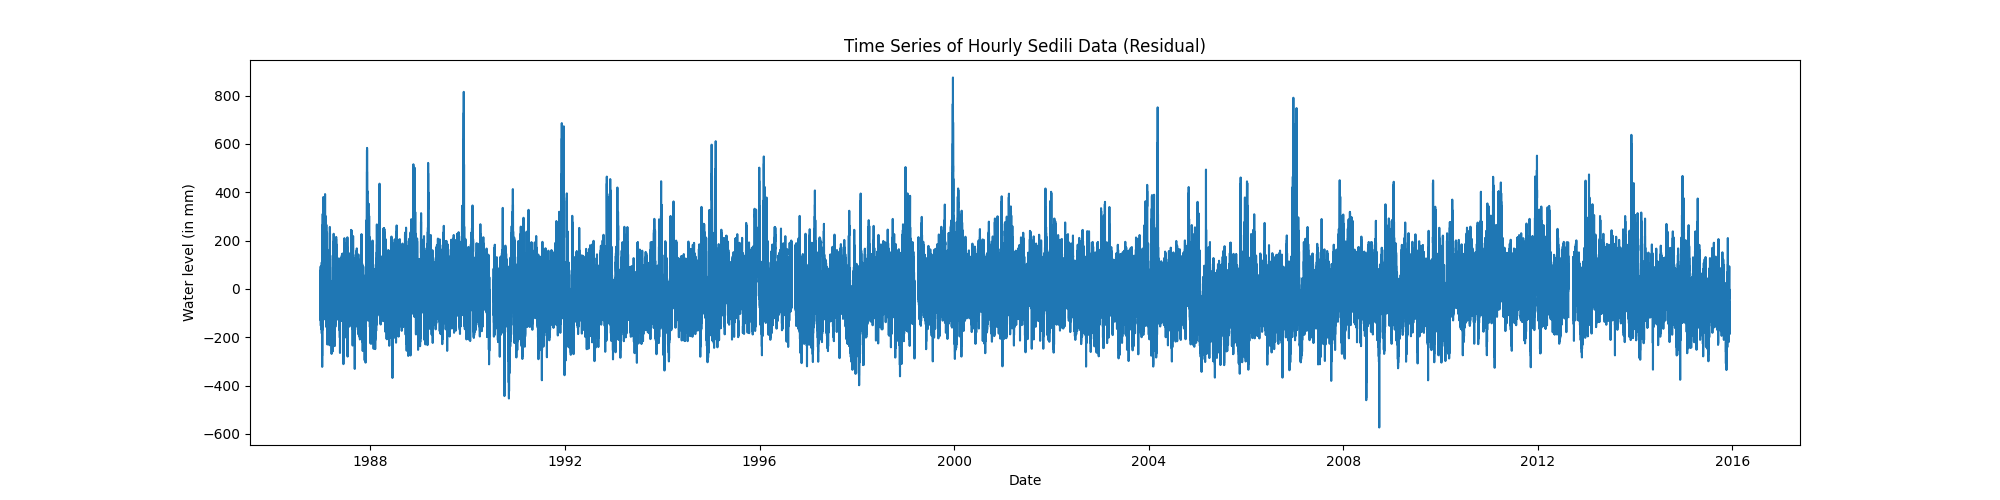
\includegraphics[width=\linewidth]{Figures/Time Series of Hourly Sedili Data (Residual).png}
        \caption{Residual Water Level at Sedili}
    \end{figure*}
    \end{itemize}
\newpage
        \item Tioman :
    \begin{itemize}
        \item Total Water Level
        \begin{figure*}[htbp]
        \centering
        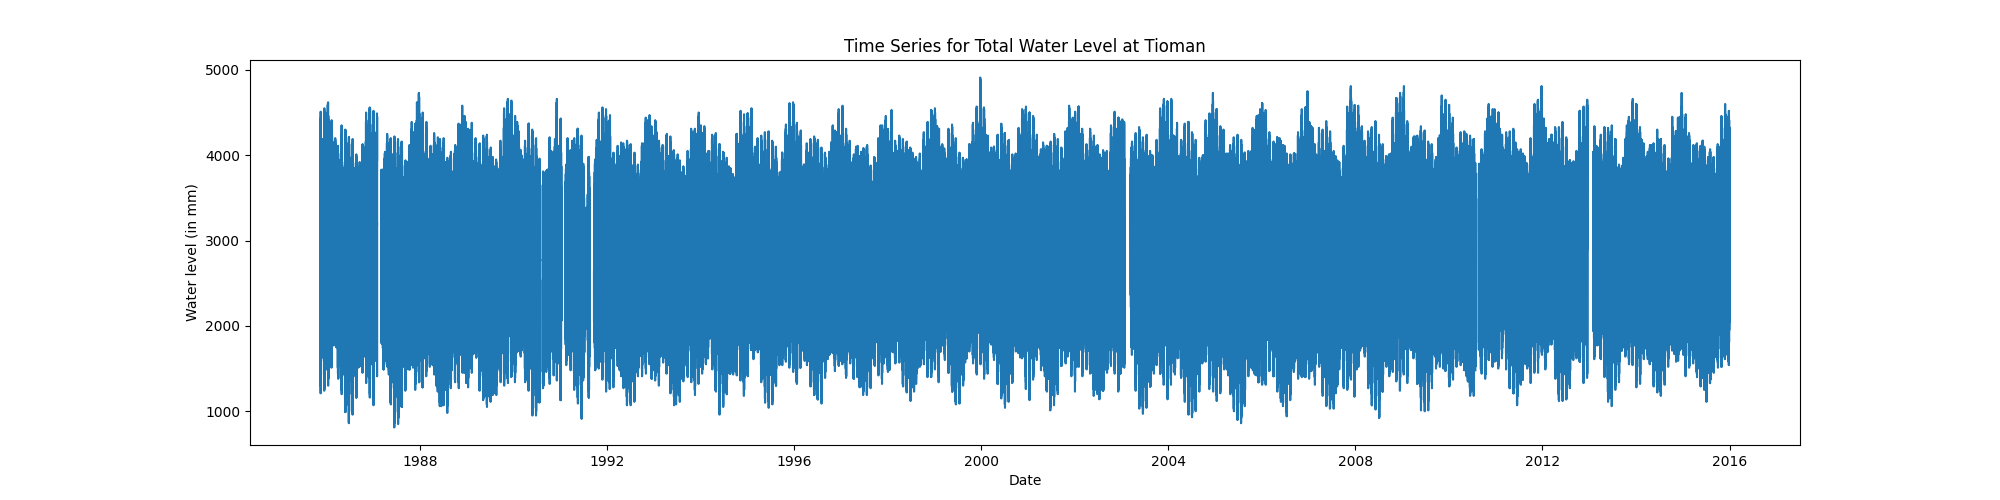
\includegraphics[width=\linewidth]{Figures/Time Series for Total Water Level at Tioman.png}
        \caption{Total Water Level at Tioman}
    \end{figure*}
    \item Predicted Water Level
        \begin{figure*}[htbp]
        \centering
        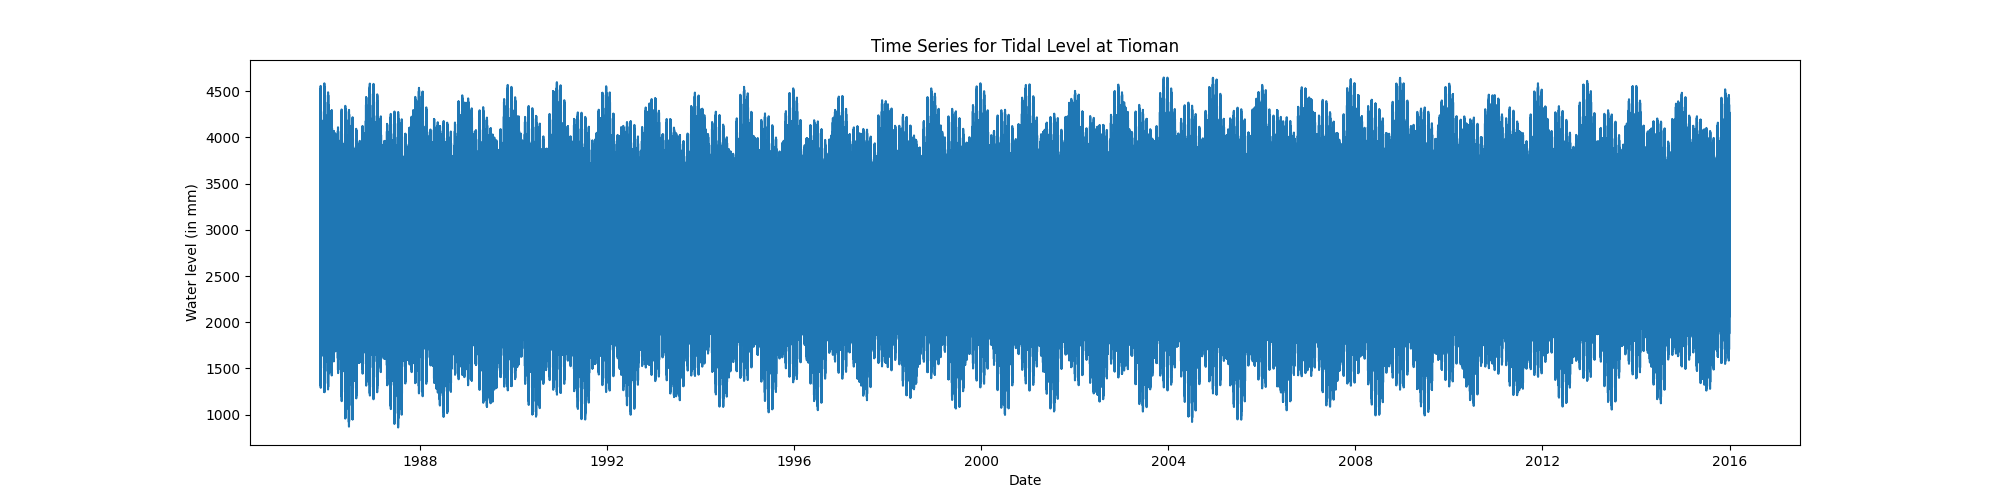
\includegraphics[width=\linewidth]{Figures/Time Series for Tidal Level at Tioman.png}
        \caption{Predicted Water Level at Tioman}
    \end{figure*}
    \item Residual Water Level
        \begin{figure*}[htbp]
        \centering
        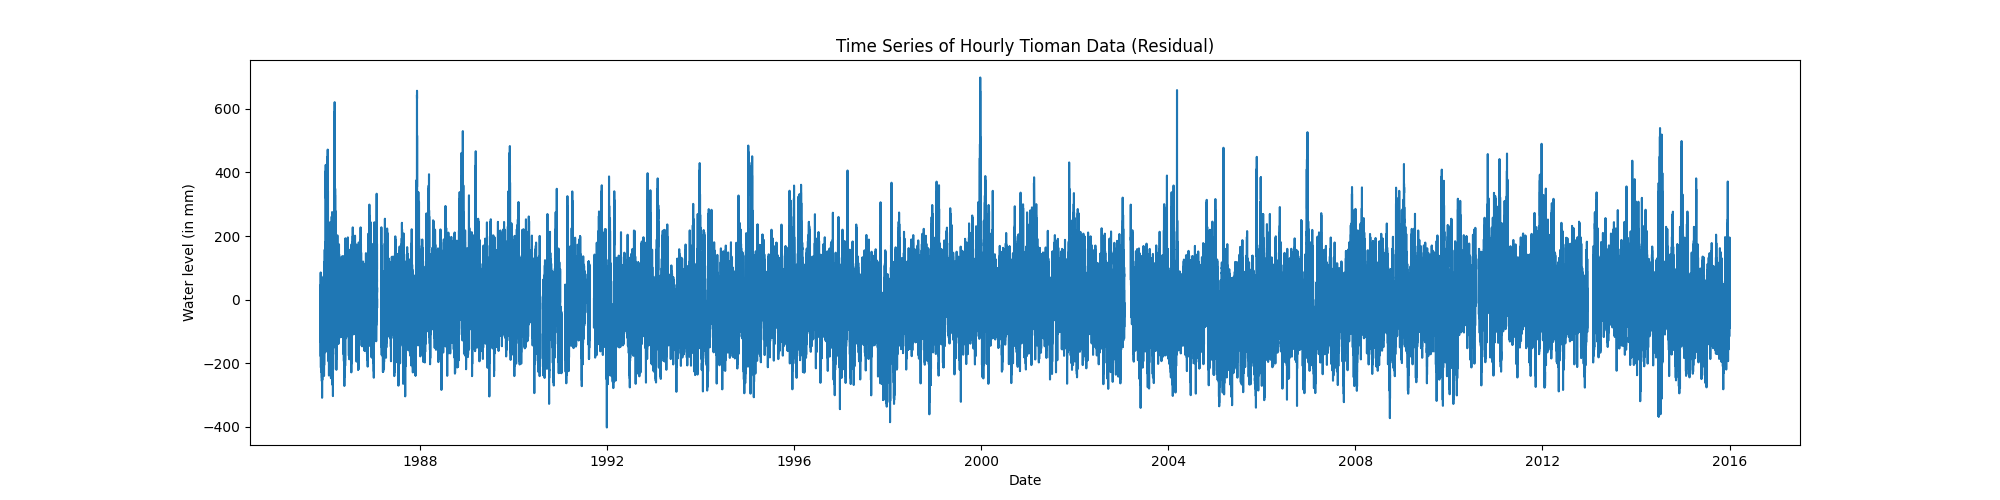
\includegraphics[width=\linewidth]{Figures/Time Series of Hourly Tioman Data (Residual).png}
        \caption{Residual Water Level at Tioman}
    \end{figure*}
    \end{itemize}
\end{itemize}

\newpage
\subsection*{Appendix C - Venn Diagrams}
\addcontentsline{toc}{subsection}{Appendix C - Venn Diagrams}
\begin{itemize}
    \item Cendering
    \begin{figure*}[htbp]
        \centering
        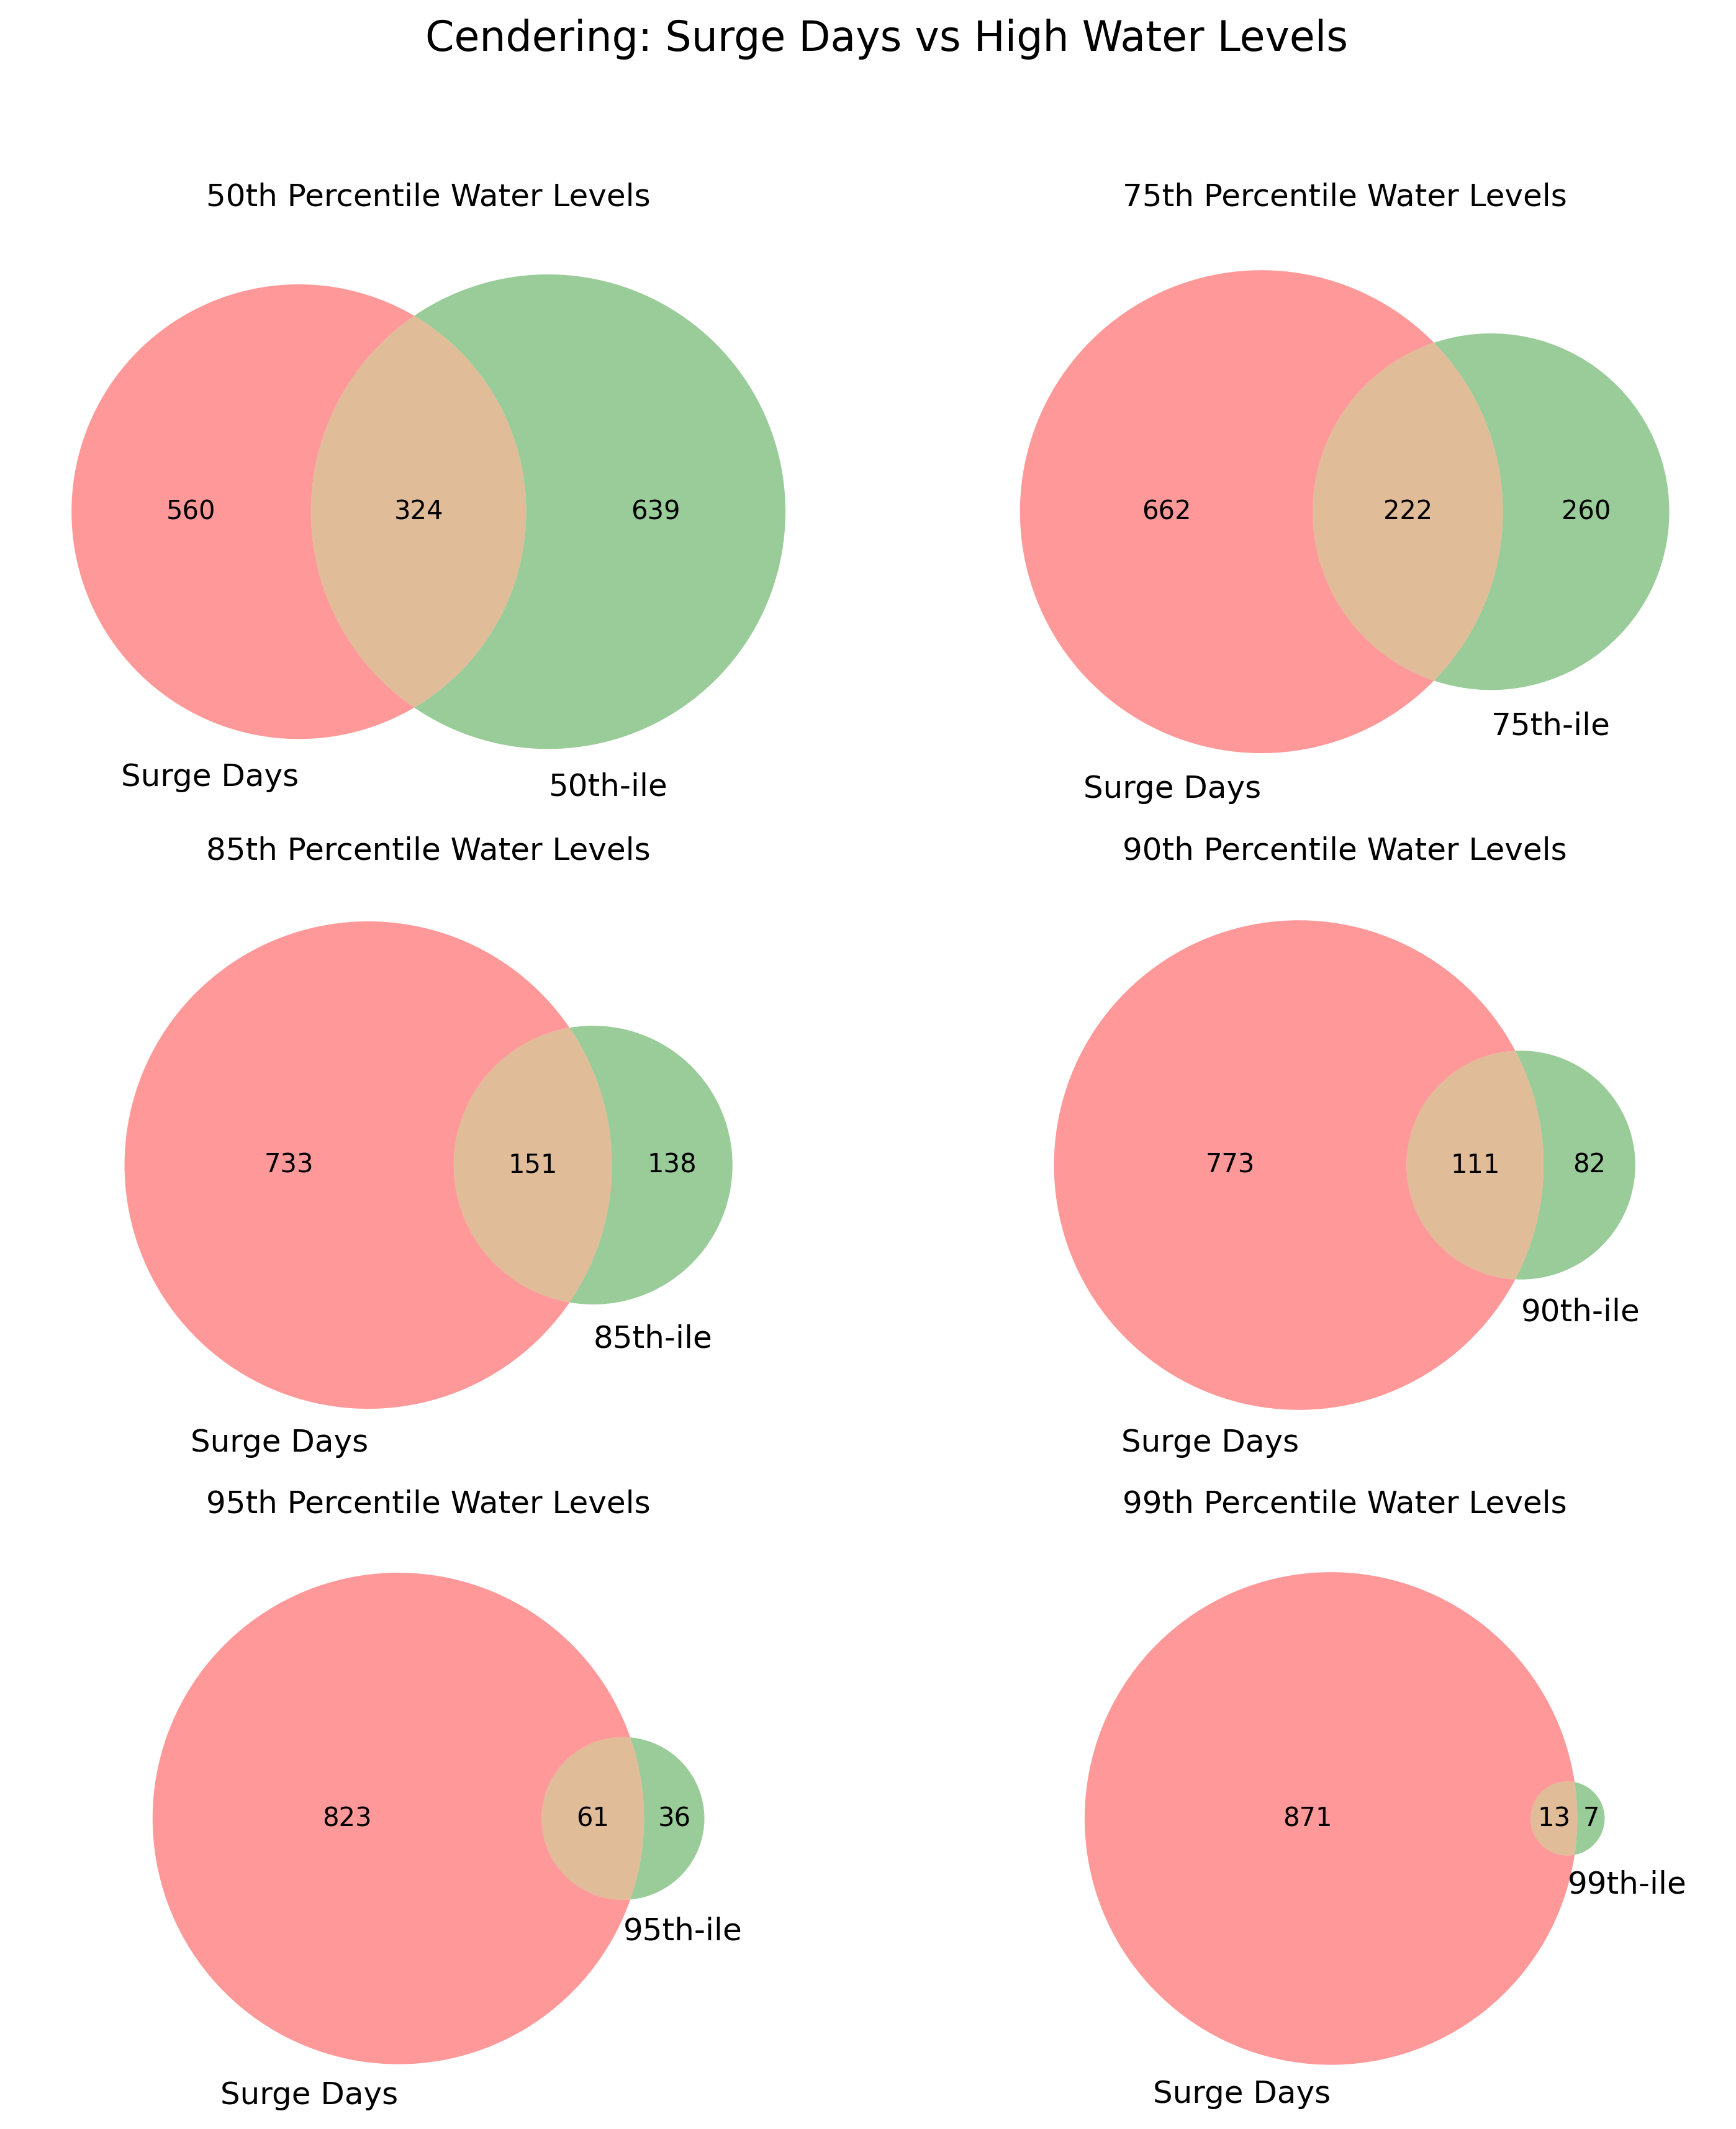
\includegraphics[width=0.8\linewidth]{Figures/cend_venn.png}
        \caption{Venn Diagram for Cendering}
    \end{figure*}
\newpage
    \item Geting
    \begin{figure*}[htbp]
        \centering
        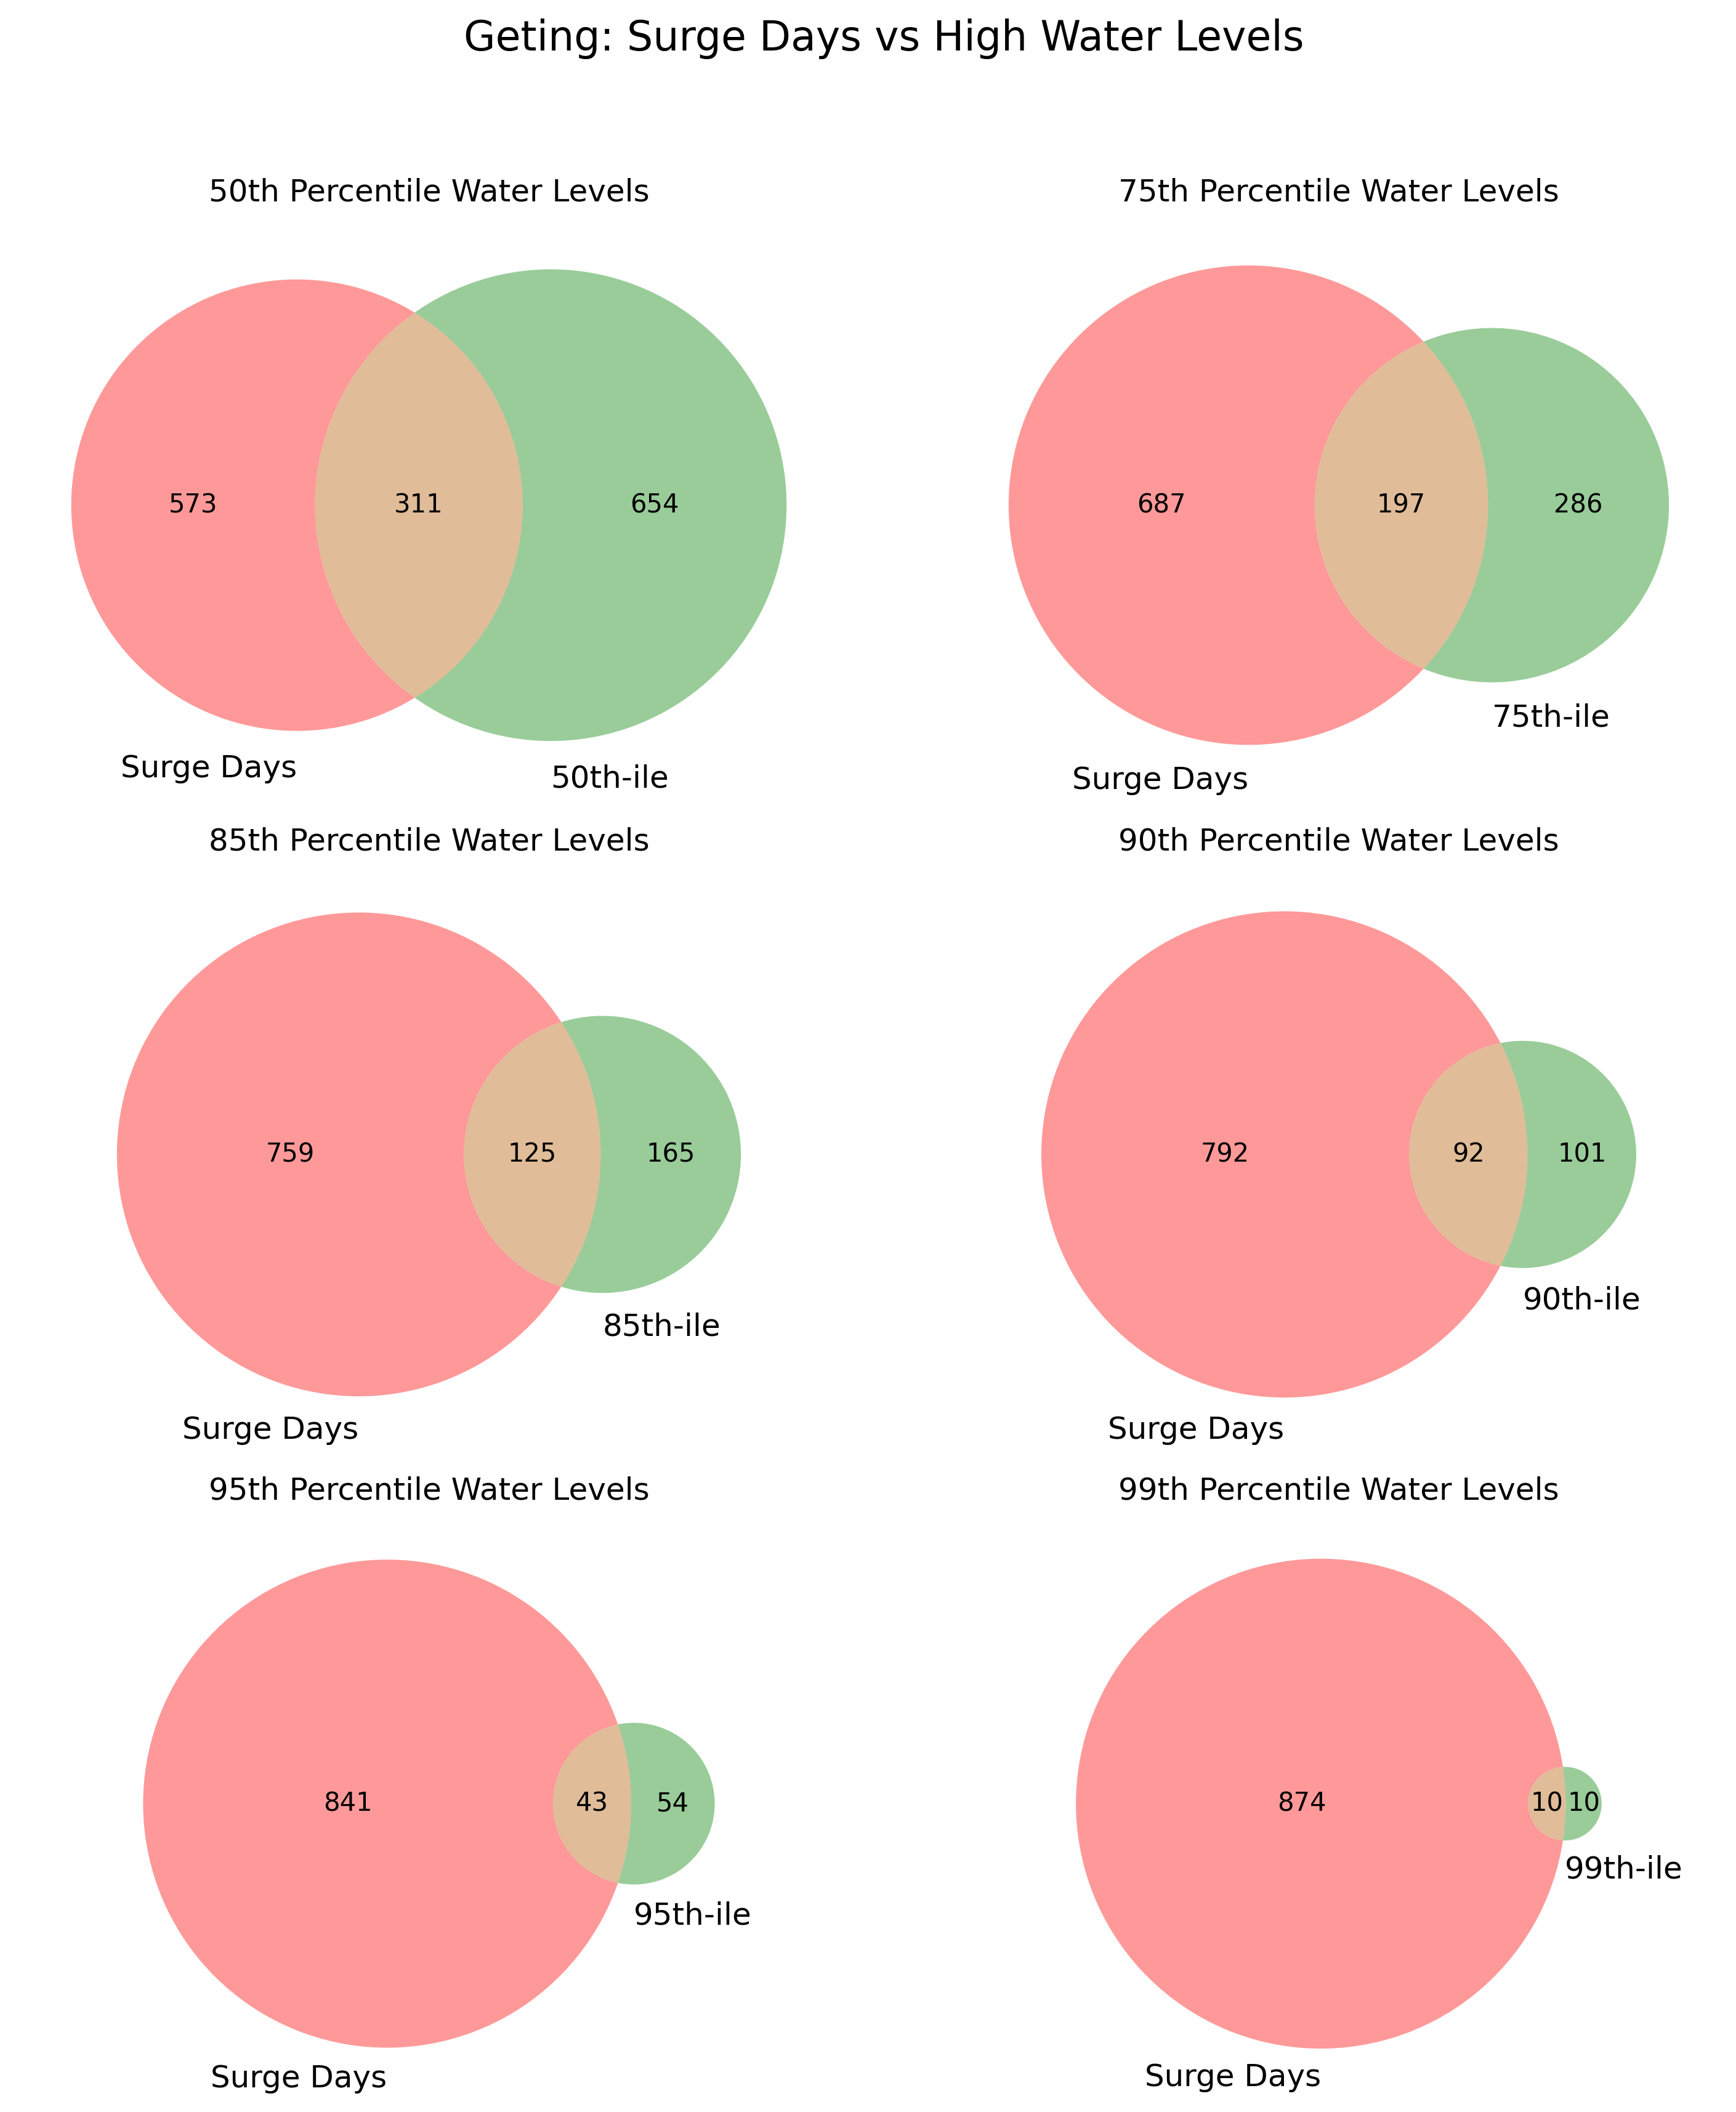
\includegraphics[width=0.8\linewidth]{Figures/geting_venn.png}
        \caption{Venn Diagram for Geting}
    \end{figure*}
\newpage
    \item Johor Baharu
    \begin{figure*}[htbp]
        \centering
        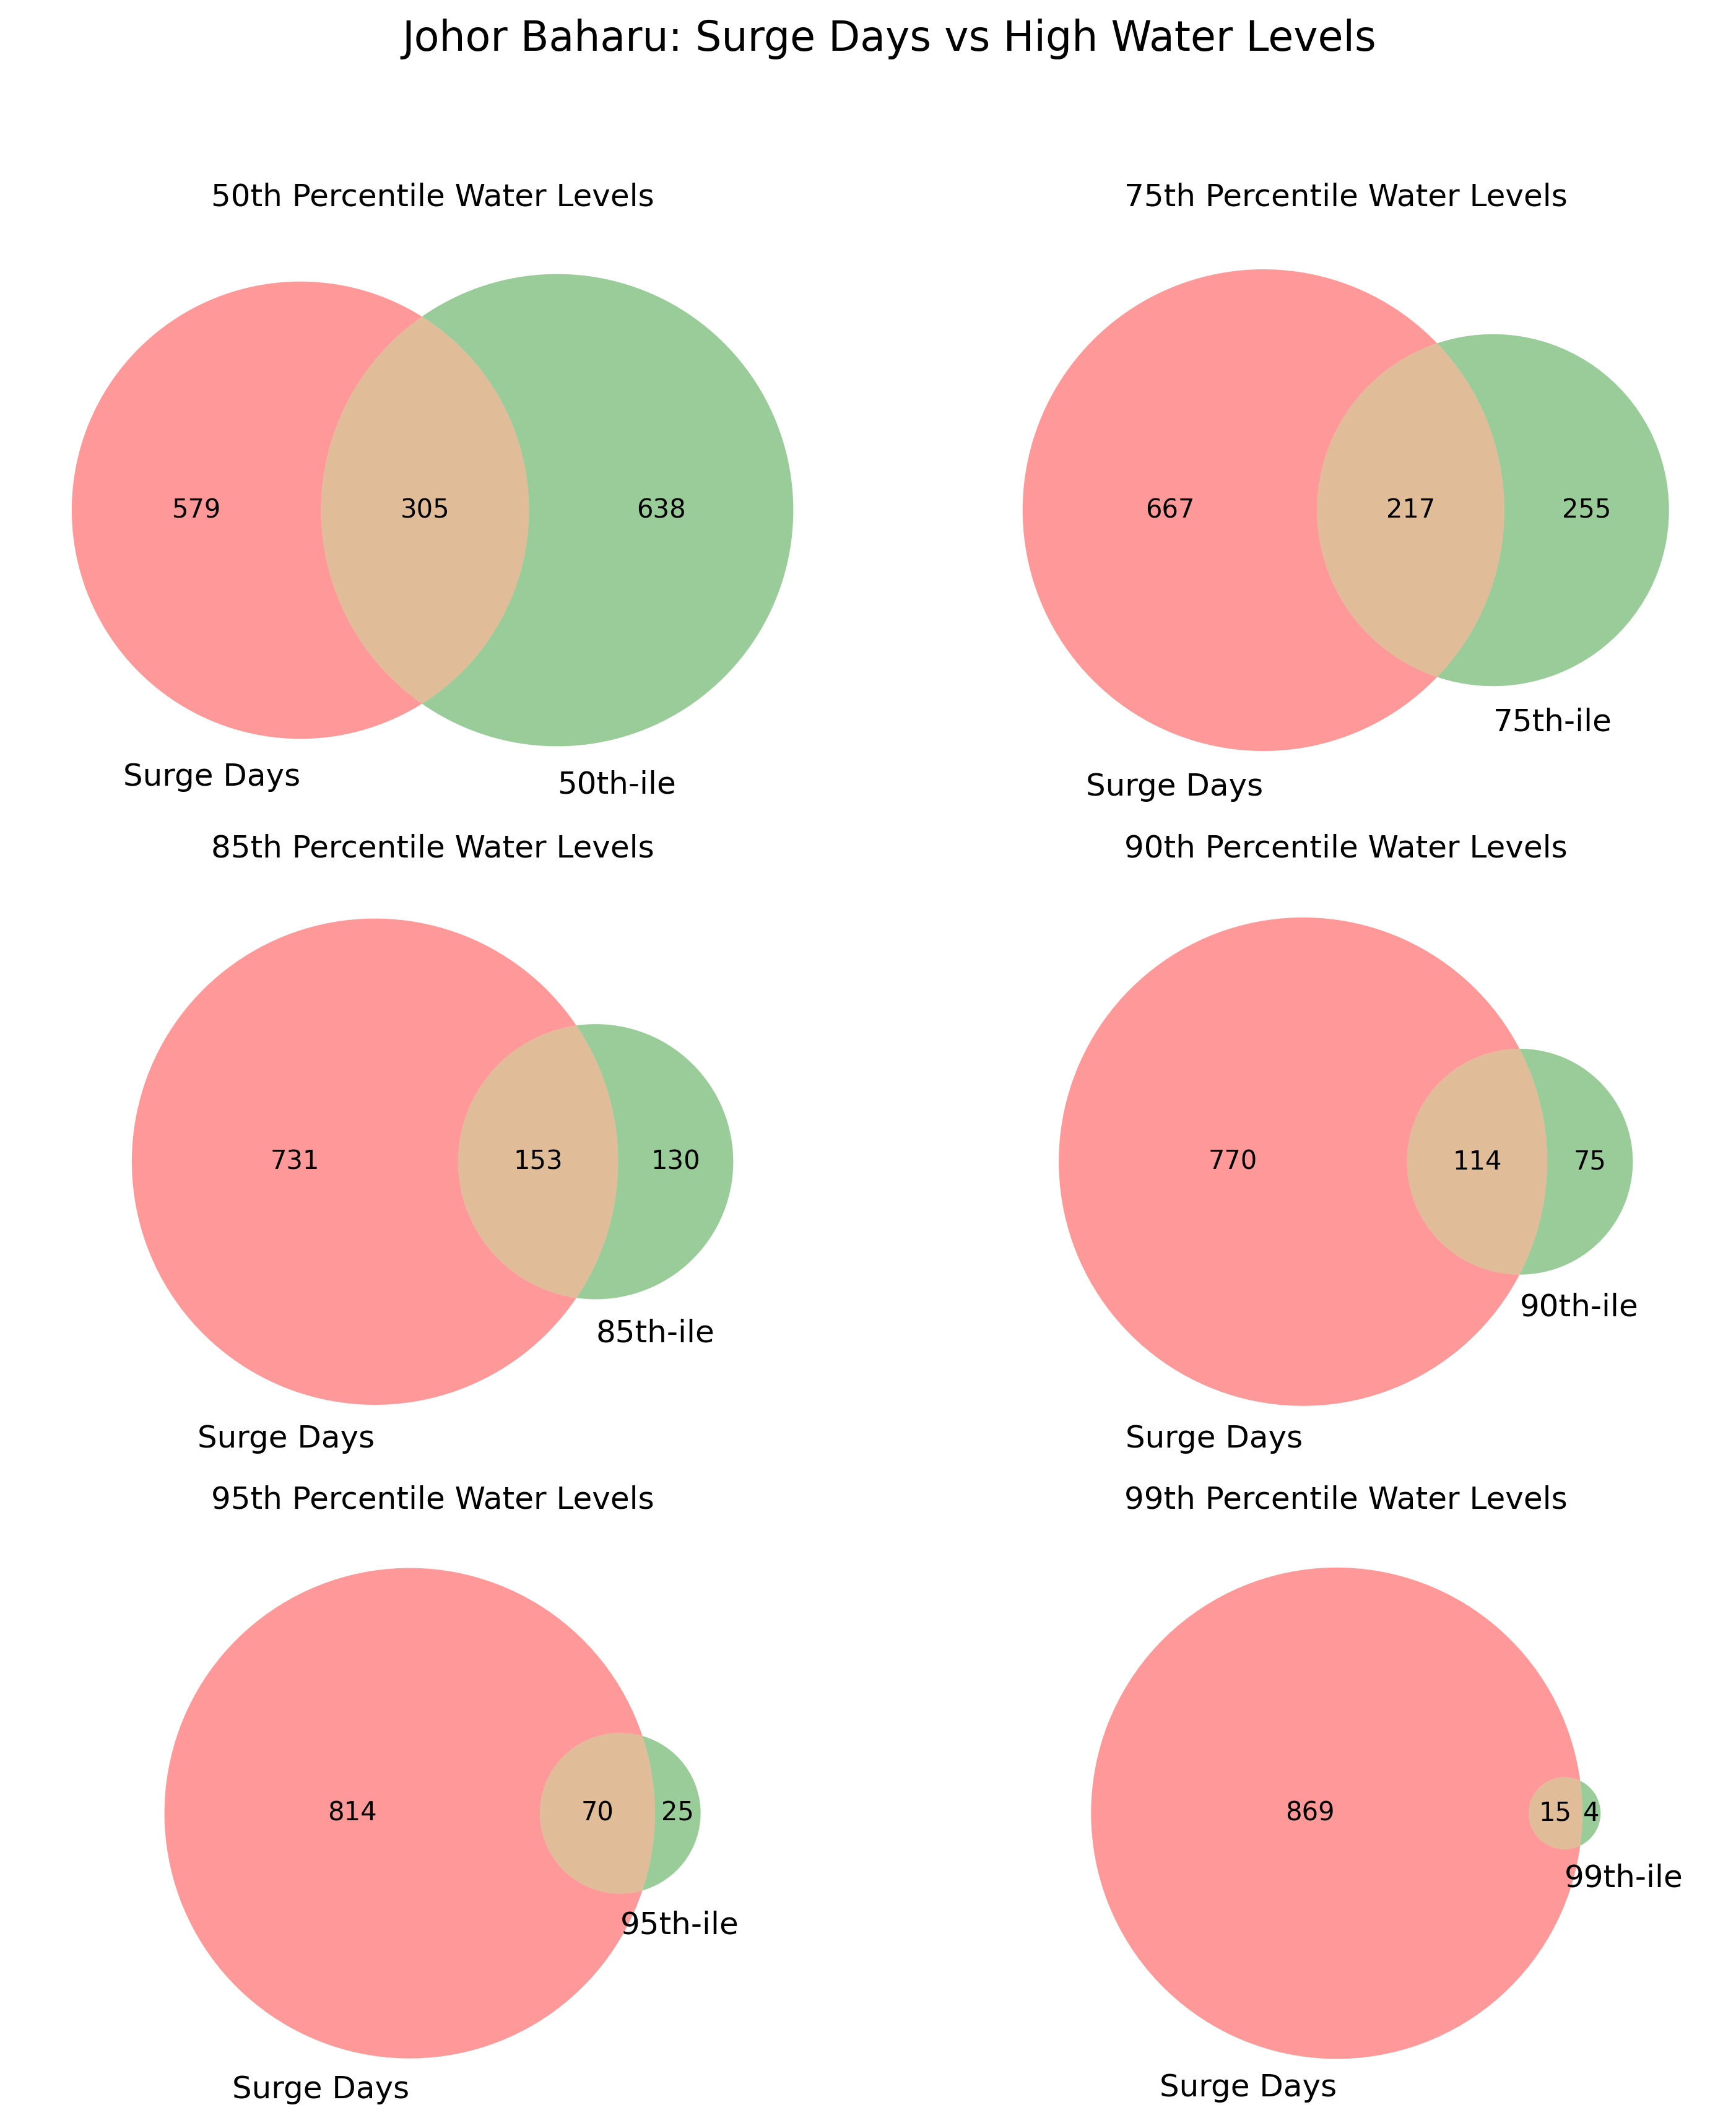
\includegraphics[width=0.8\linewidth]{Figures/jb_venn.png}
        \caption{Venn Diagram for Johor Baharu}
    \end{figure*}
\newpage
    \item Sedili
    \begin{figure*}[htbp]
        \centering
        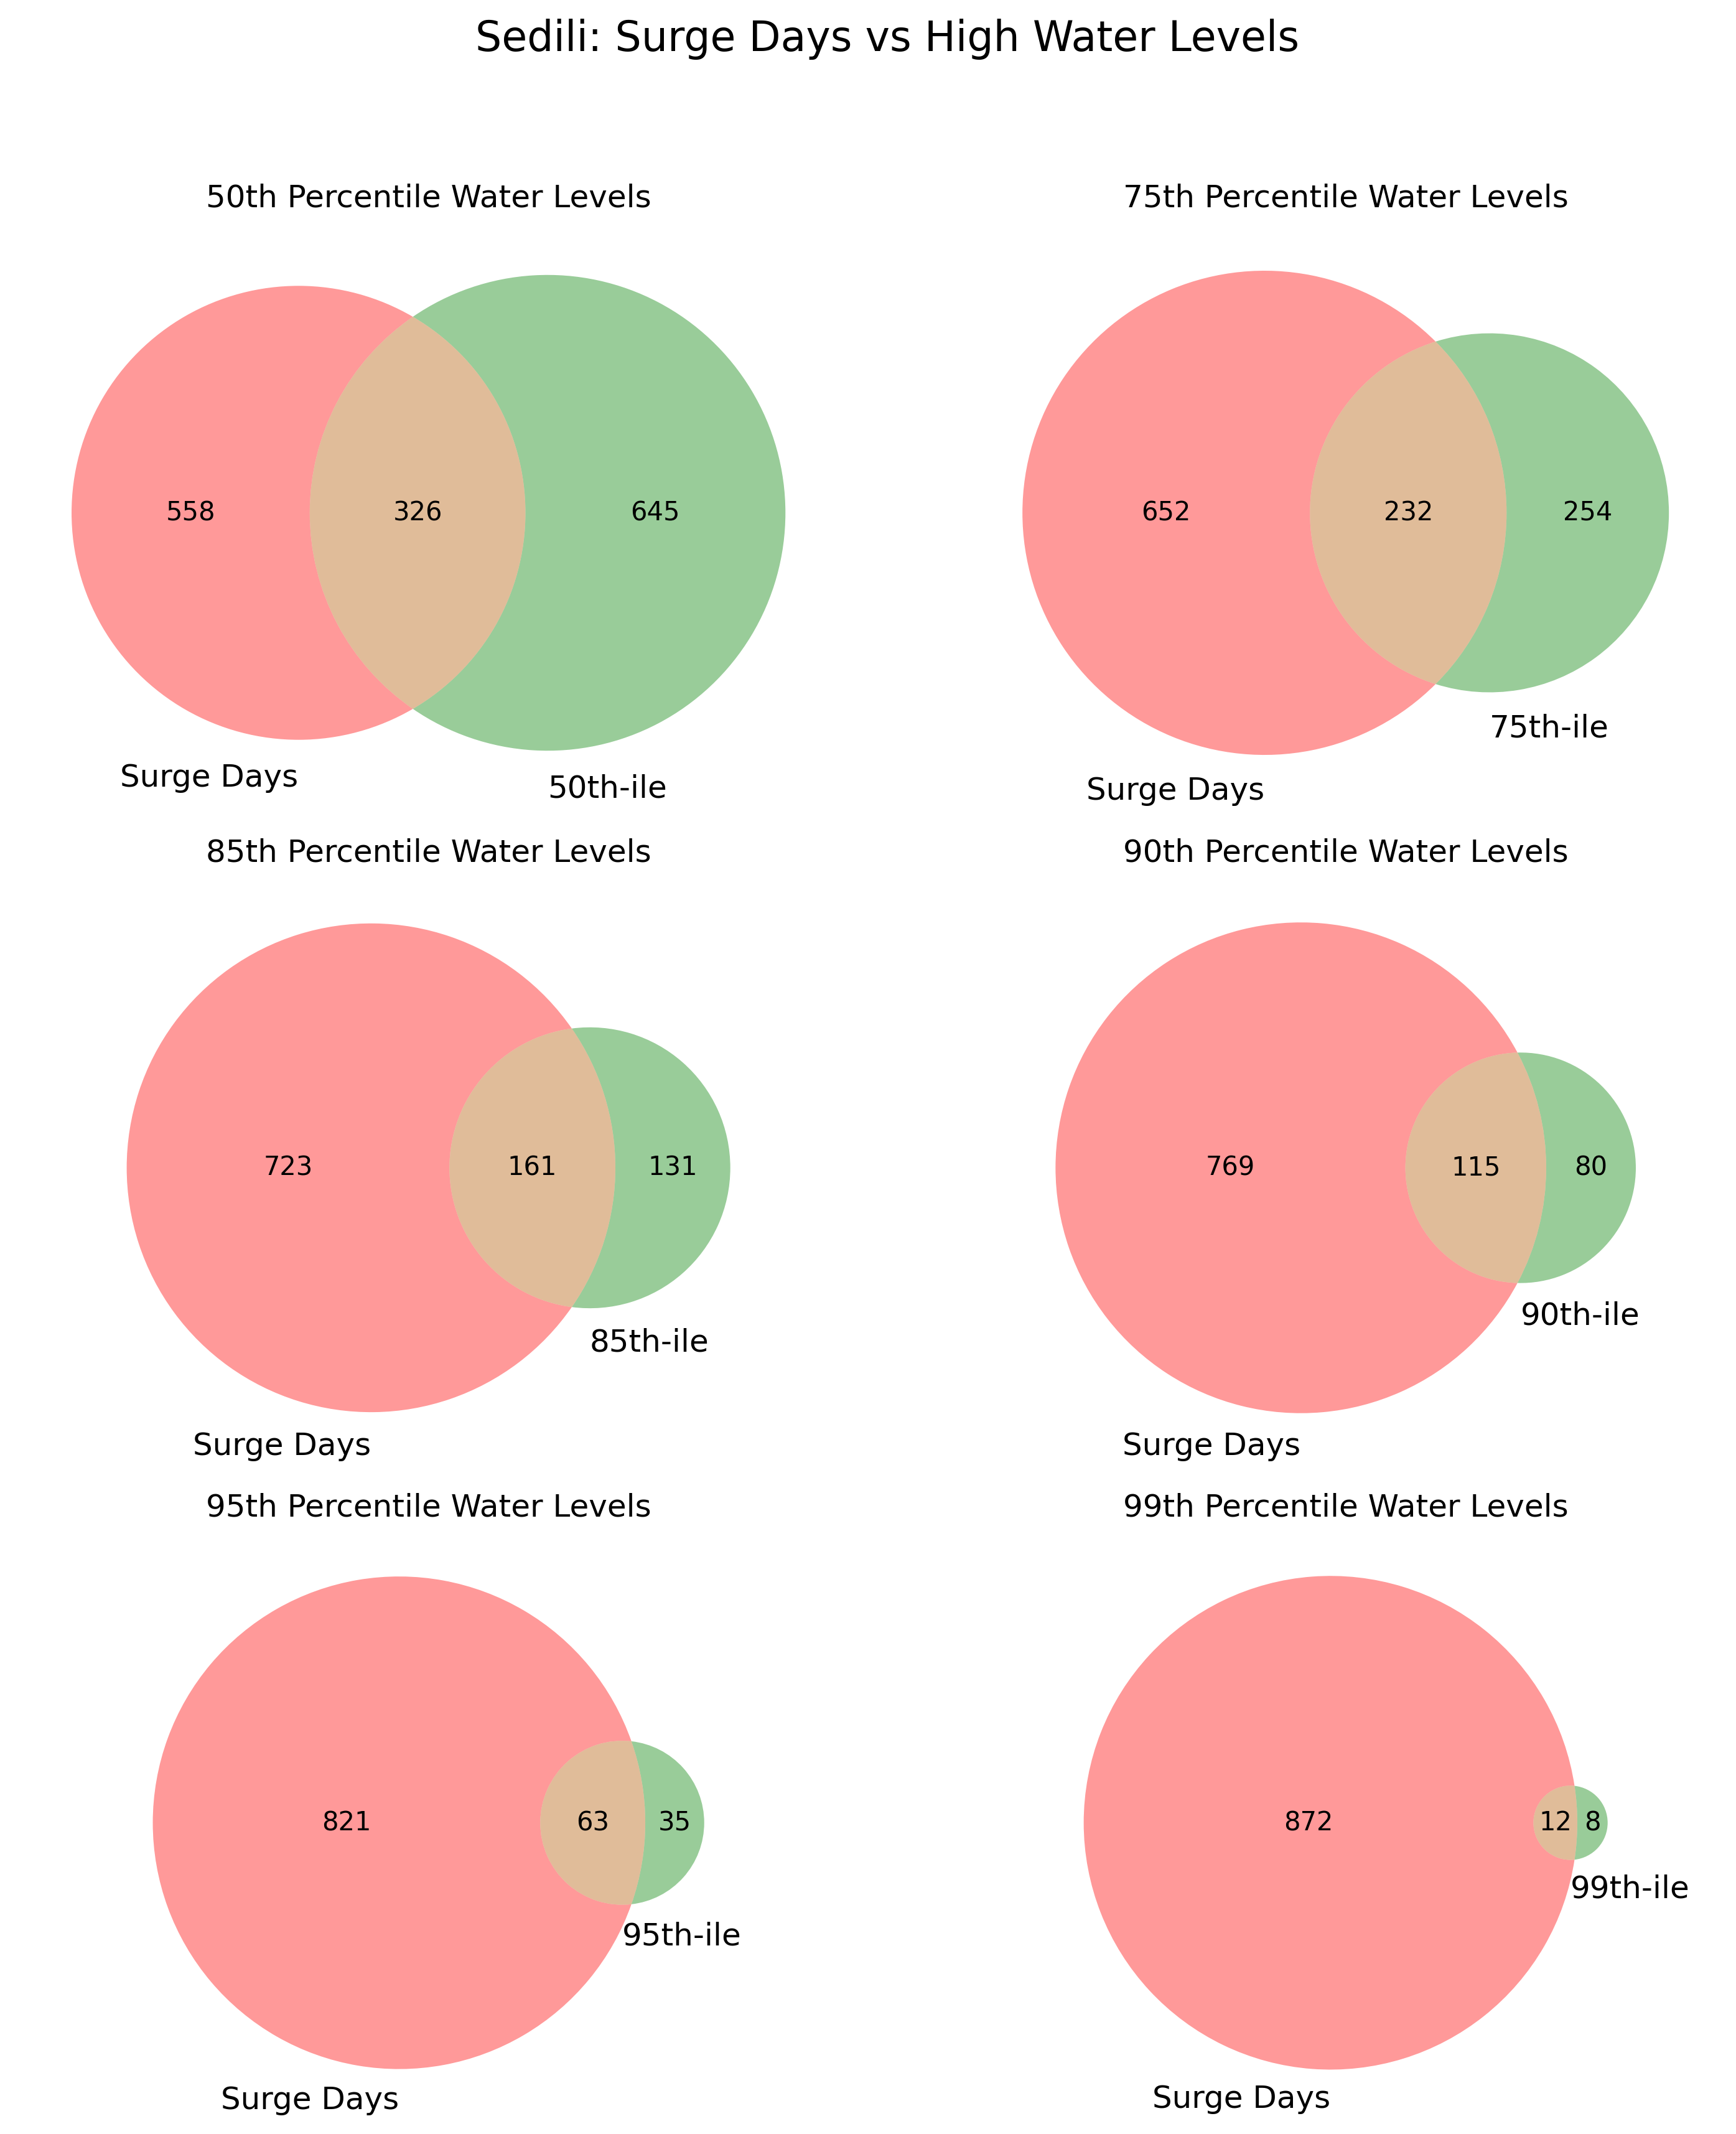
\includegraphics[width=0.8\linewidth]{Figures/sedili_venn.png}
        \caption{Venn Diagram for Sedili}
    \end{figure*}
\newpage
    \item Tioman
    \begin{figure*}[htbp]
        \centering
        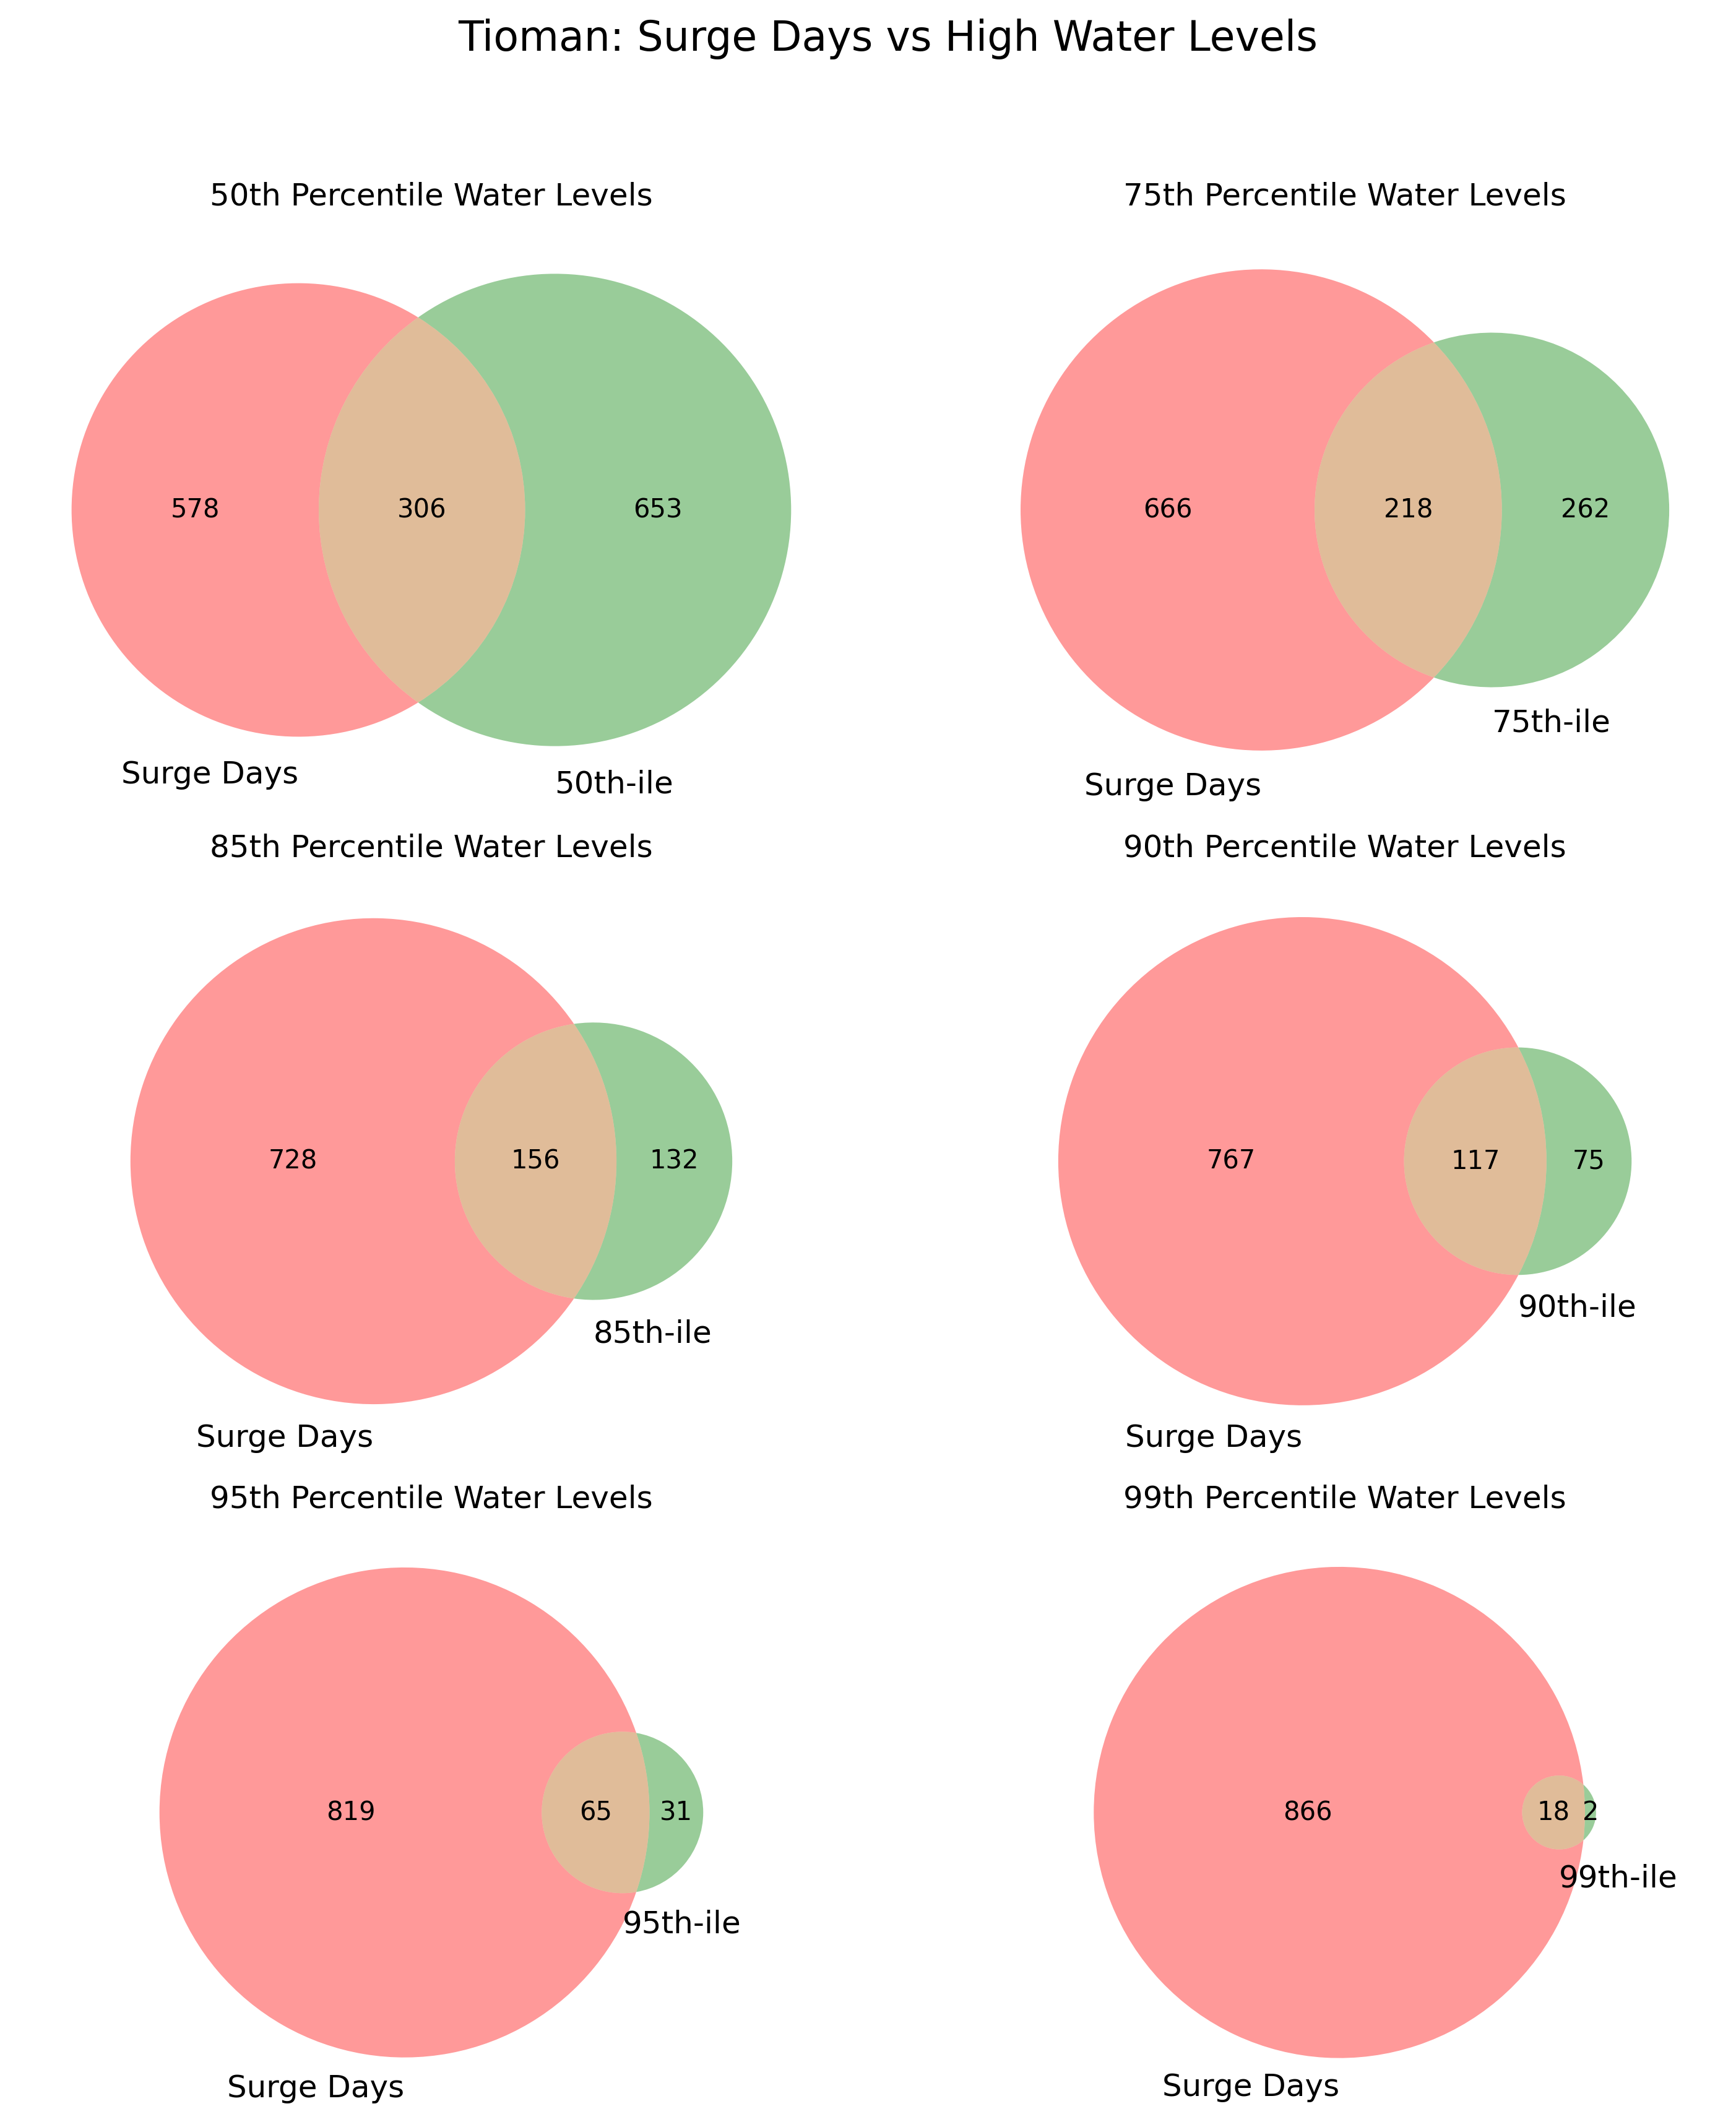
\includegraphics[width=0.8\linewidth]{Figures/tioman_venn.png}
        \caption{Venn Diagram for Tioman}
    \end{figure*}
\end{itemize}

\newpage
\subsection*{Appendix D - Cross Validation}
\addcontentsline{toc}{subsection}{Appendix D - Cross Validation}
\begin{itemize}
    \item Residual Daily Maximum Predictions
    \begin{figure*}[htbp]
        \centering
        \includegraphics[width=\linewidth]{Figures/all_locs_model_trained.png}
        \caption{Residual Daily Maximum Predictions for Malaysian Tide Gauges}
    \end{figure*}
\newpage
    \item Hind-cast graphs with different samples from the distribution between 1985-1990
    \begin{itemize}
        \item Cendering
        \begin{figure*}[htbp]
        \centering
        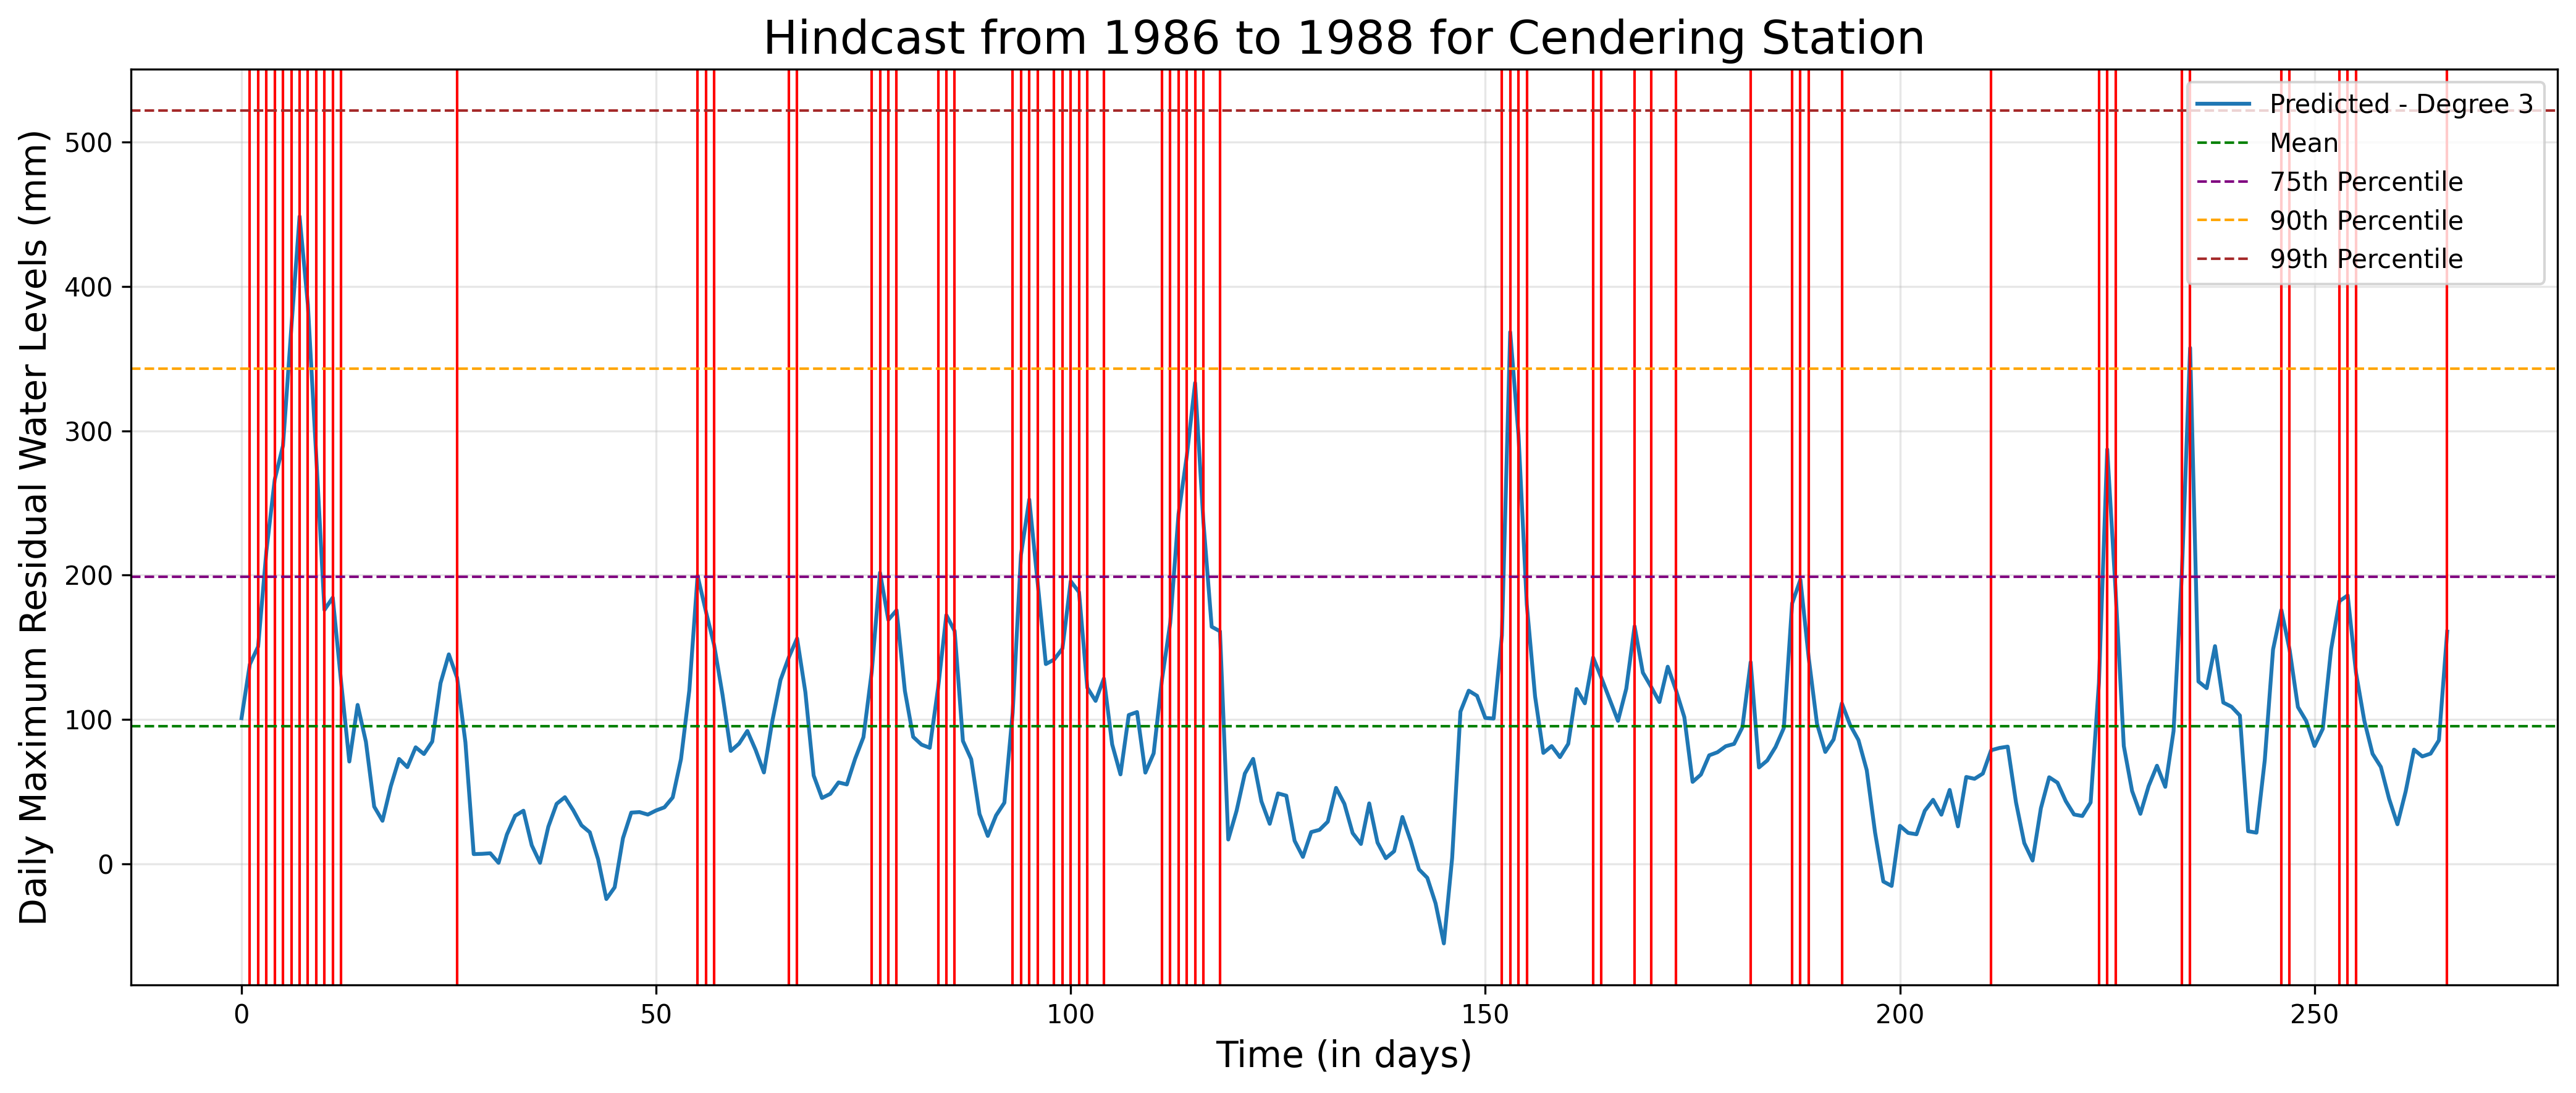
\includegraphics[width=0.9\linewidth]{Figures/HIndcast_1984_1986_cendering_SD.png}
        \caption{Hindcast for Cendering}
    \end{figure*}
    \item Geting
        \begin{figure*}[htbp]
        \centering
        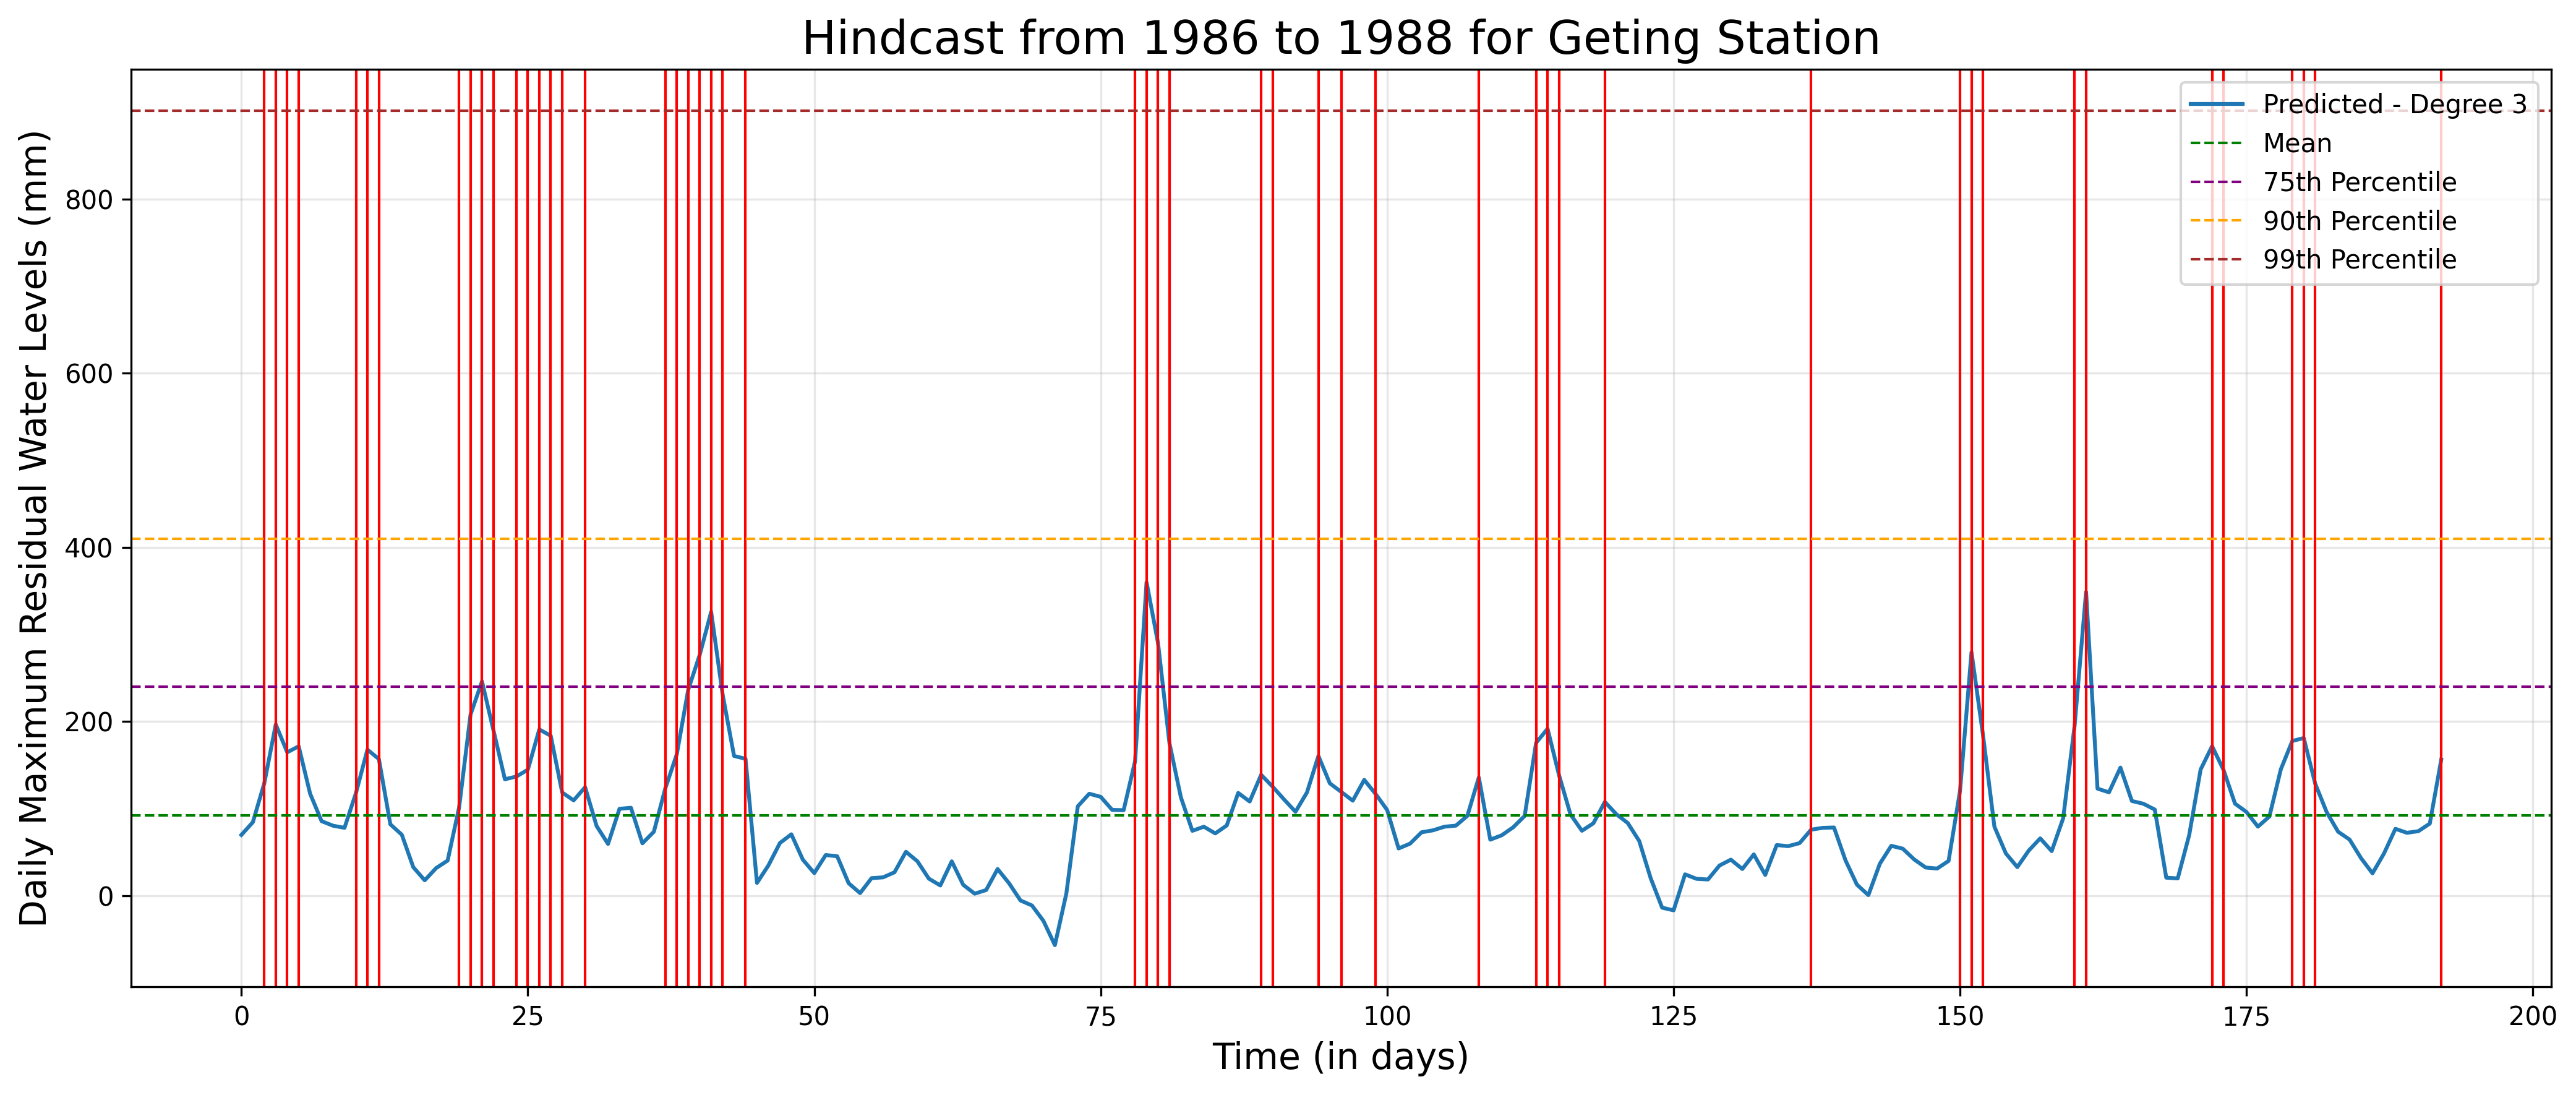
\includegraphics[width=0.9\linewidth]{Figures/HIndcast_1984_1986_geting_SD.png}
        \caption{Hindcast for Geting}
    \end{figure*}
\newpage
    \item Kuantan
        \begin{figure*}[htbp]
        \centering
        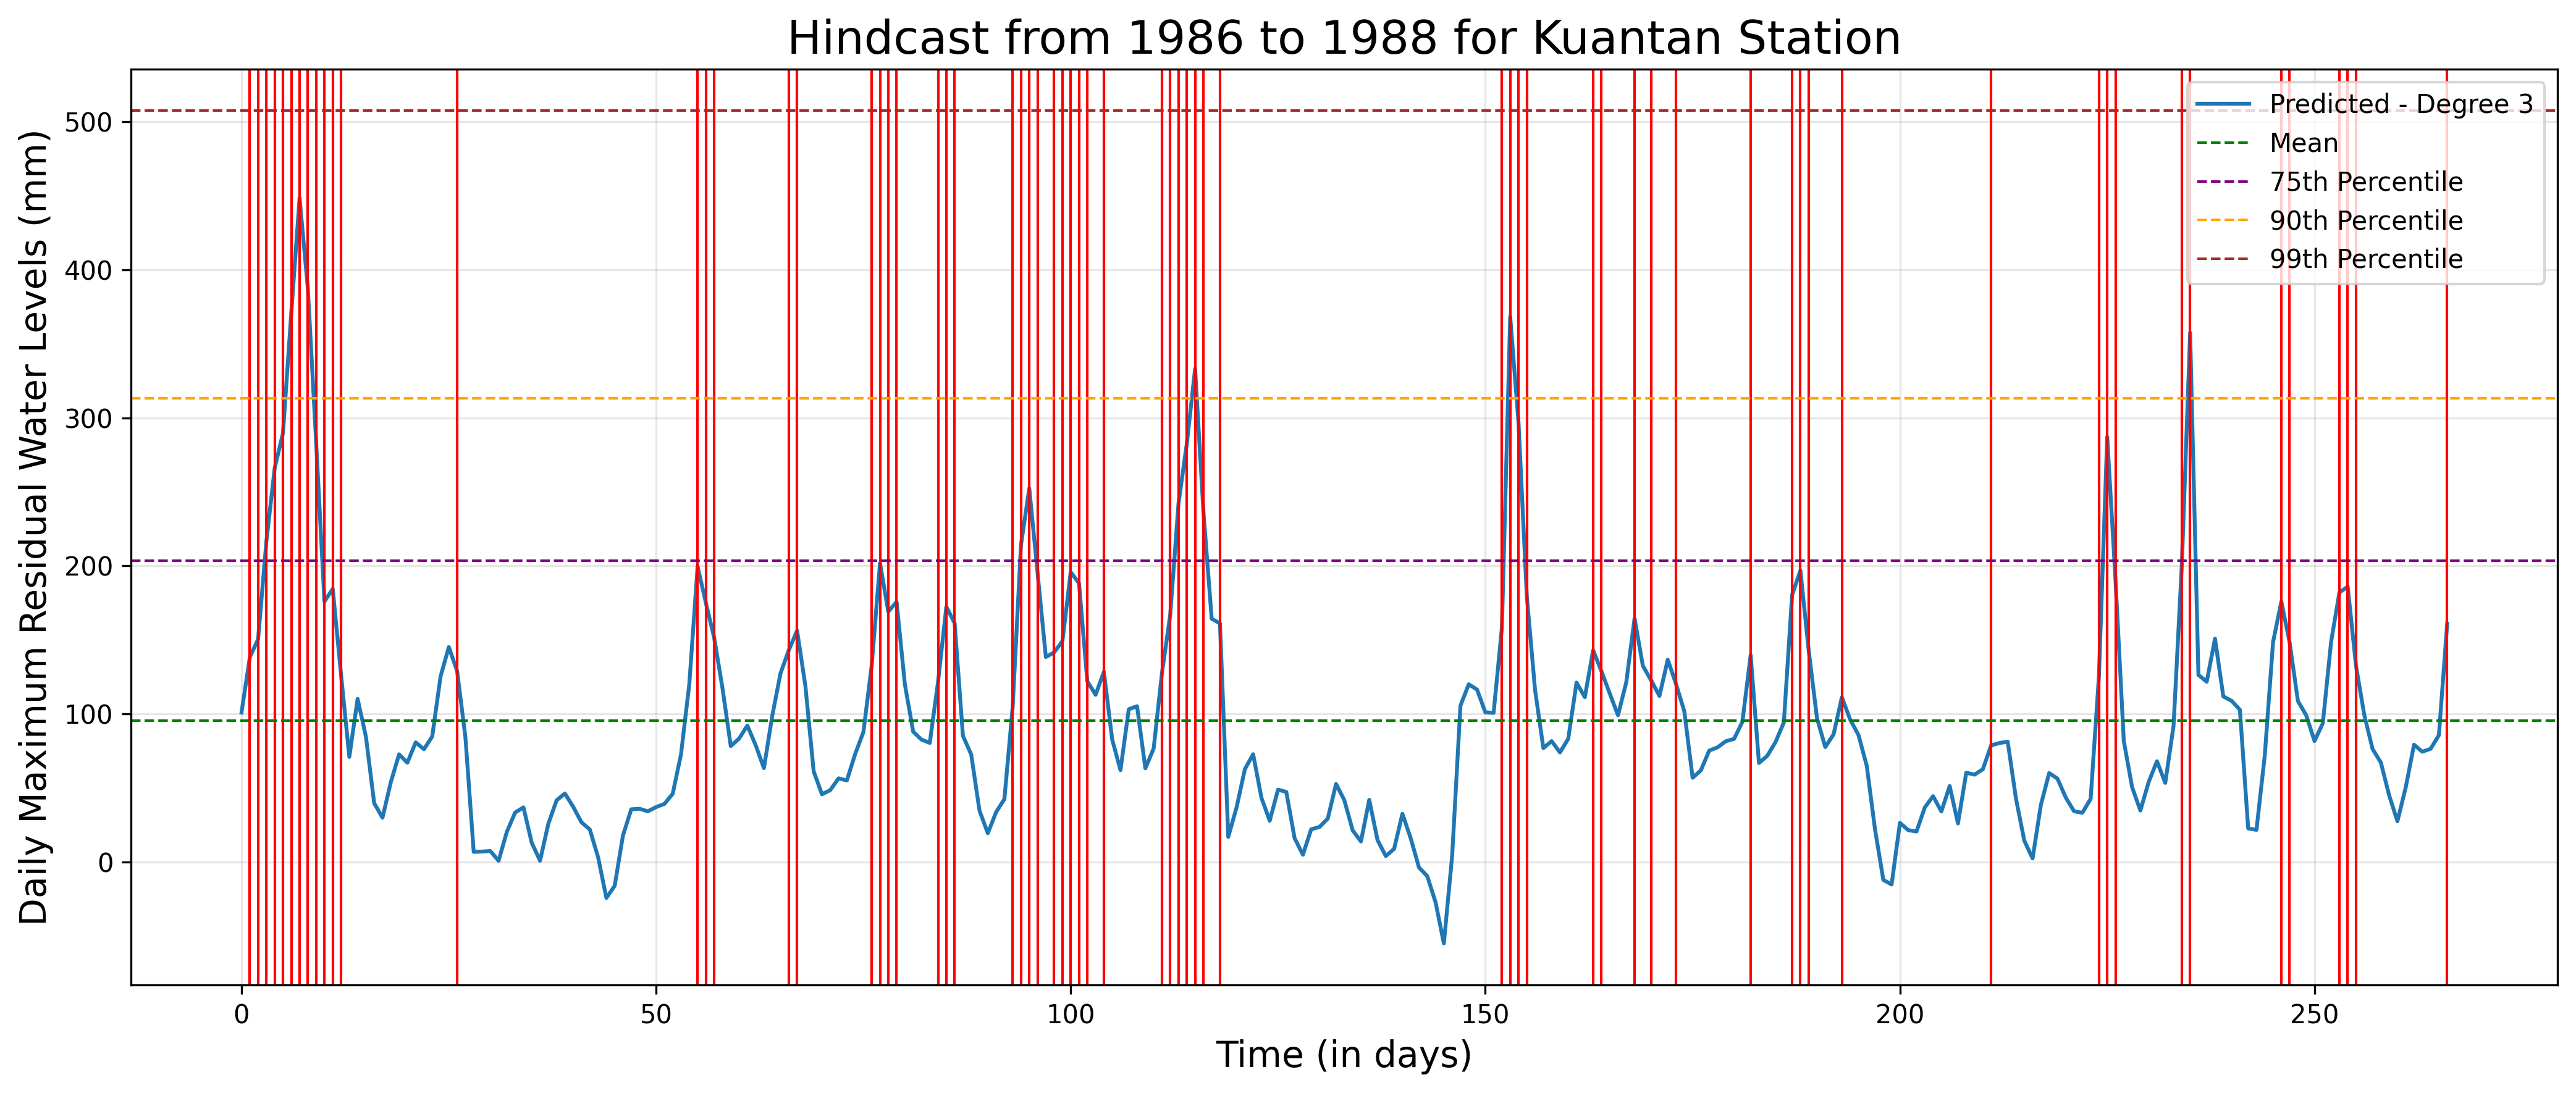
\includegraphics[width=0.9\linewidth]{Figures/HIndcast_1984_1986_kuantan_SD.png}
        \caption{Hindcast for Kuantan}
    \end{figure*}
    \item Johor Baharu
        \begin{figure*}[htbp]
        \centering
        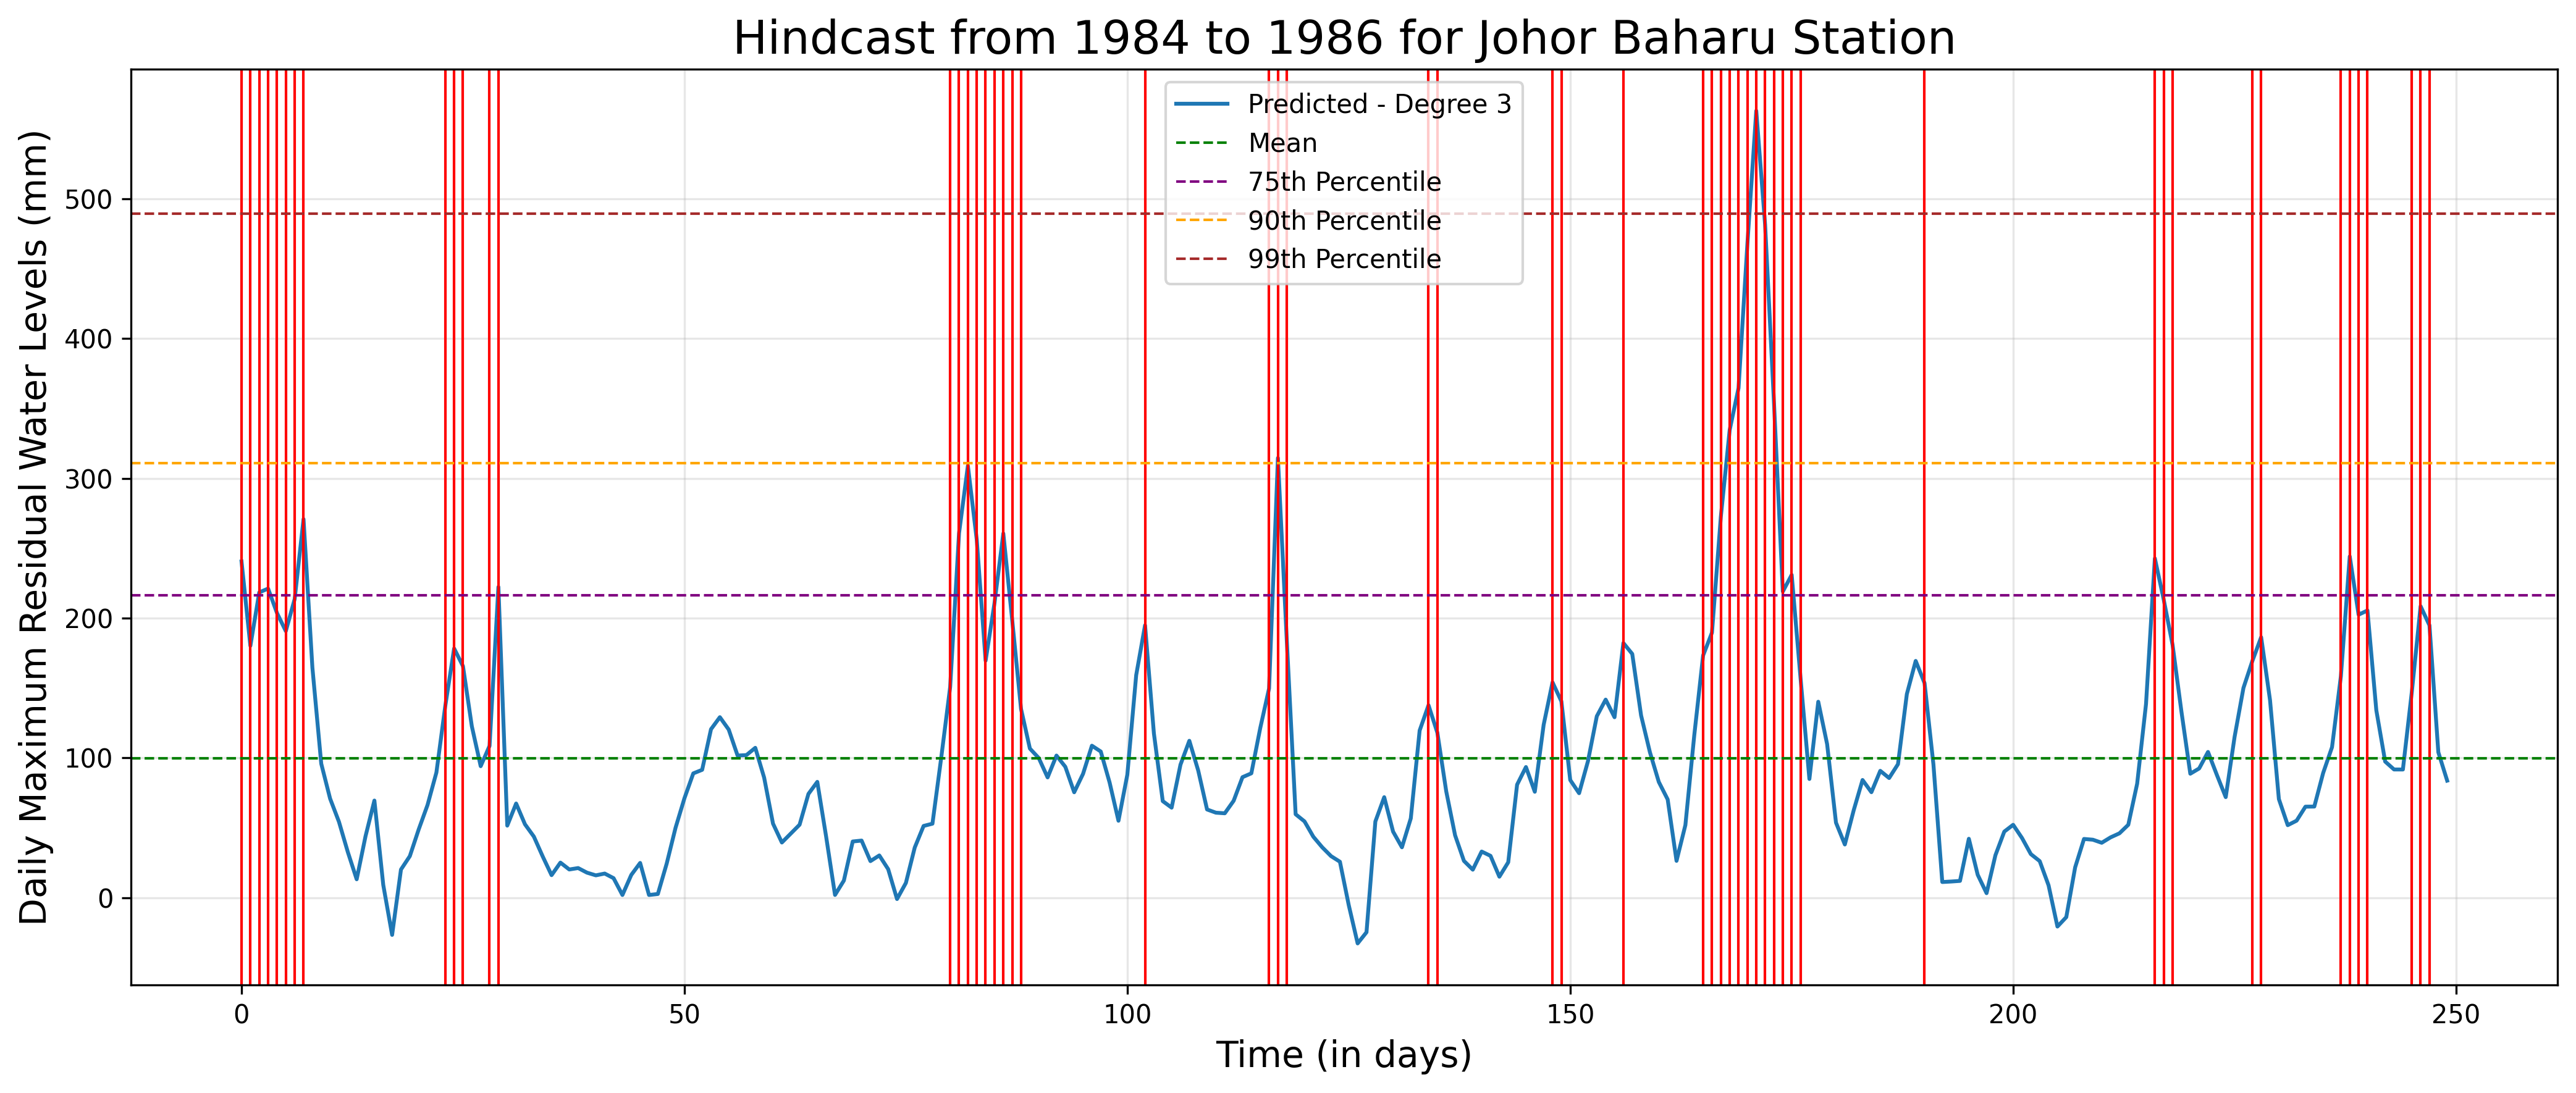
\includegraphics[width=0.9\linewidth]{Figures/HIndcast_1984_1986_JB_SD.png}
        \caption{Hindcast for Johor Baharu}
    \end{figure*}
\newpage
    \item Sedili
        \begin{figure*}[htbp]
        \centering
        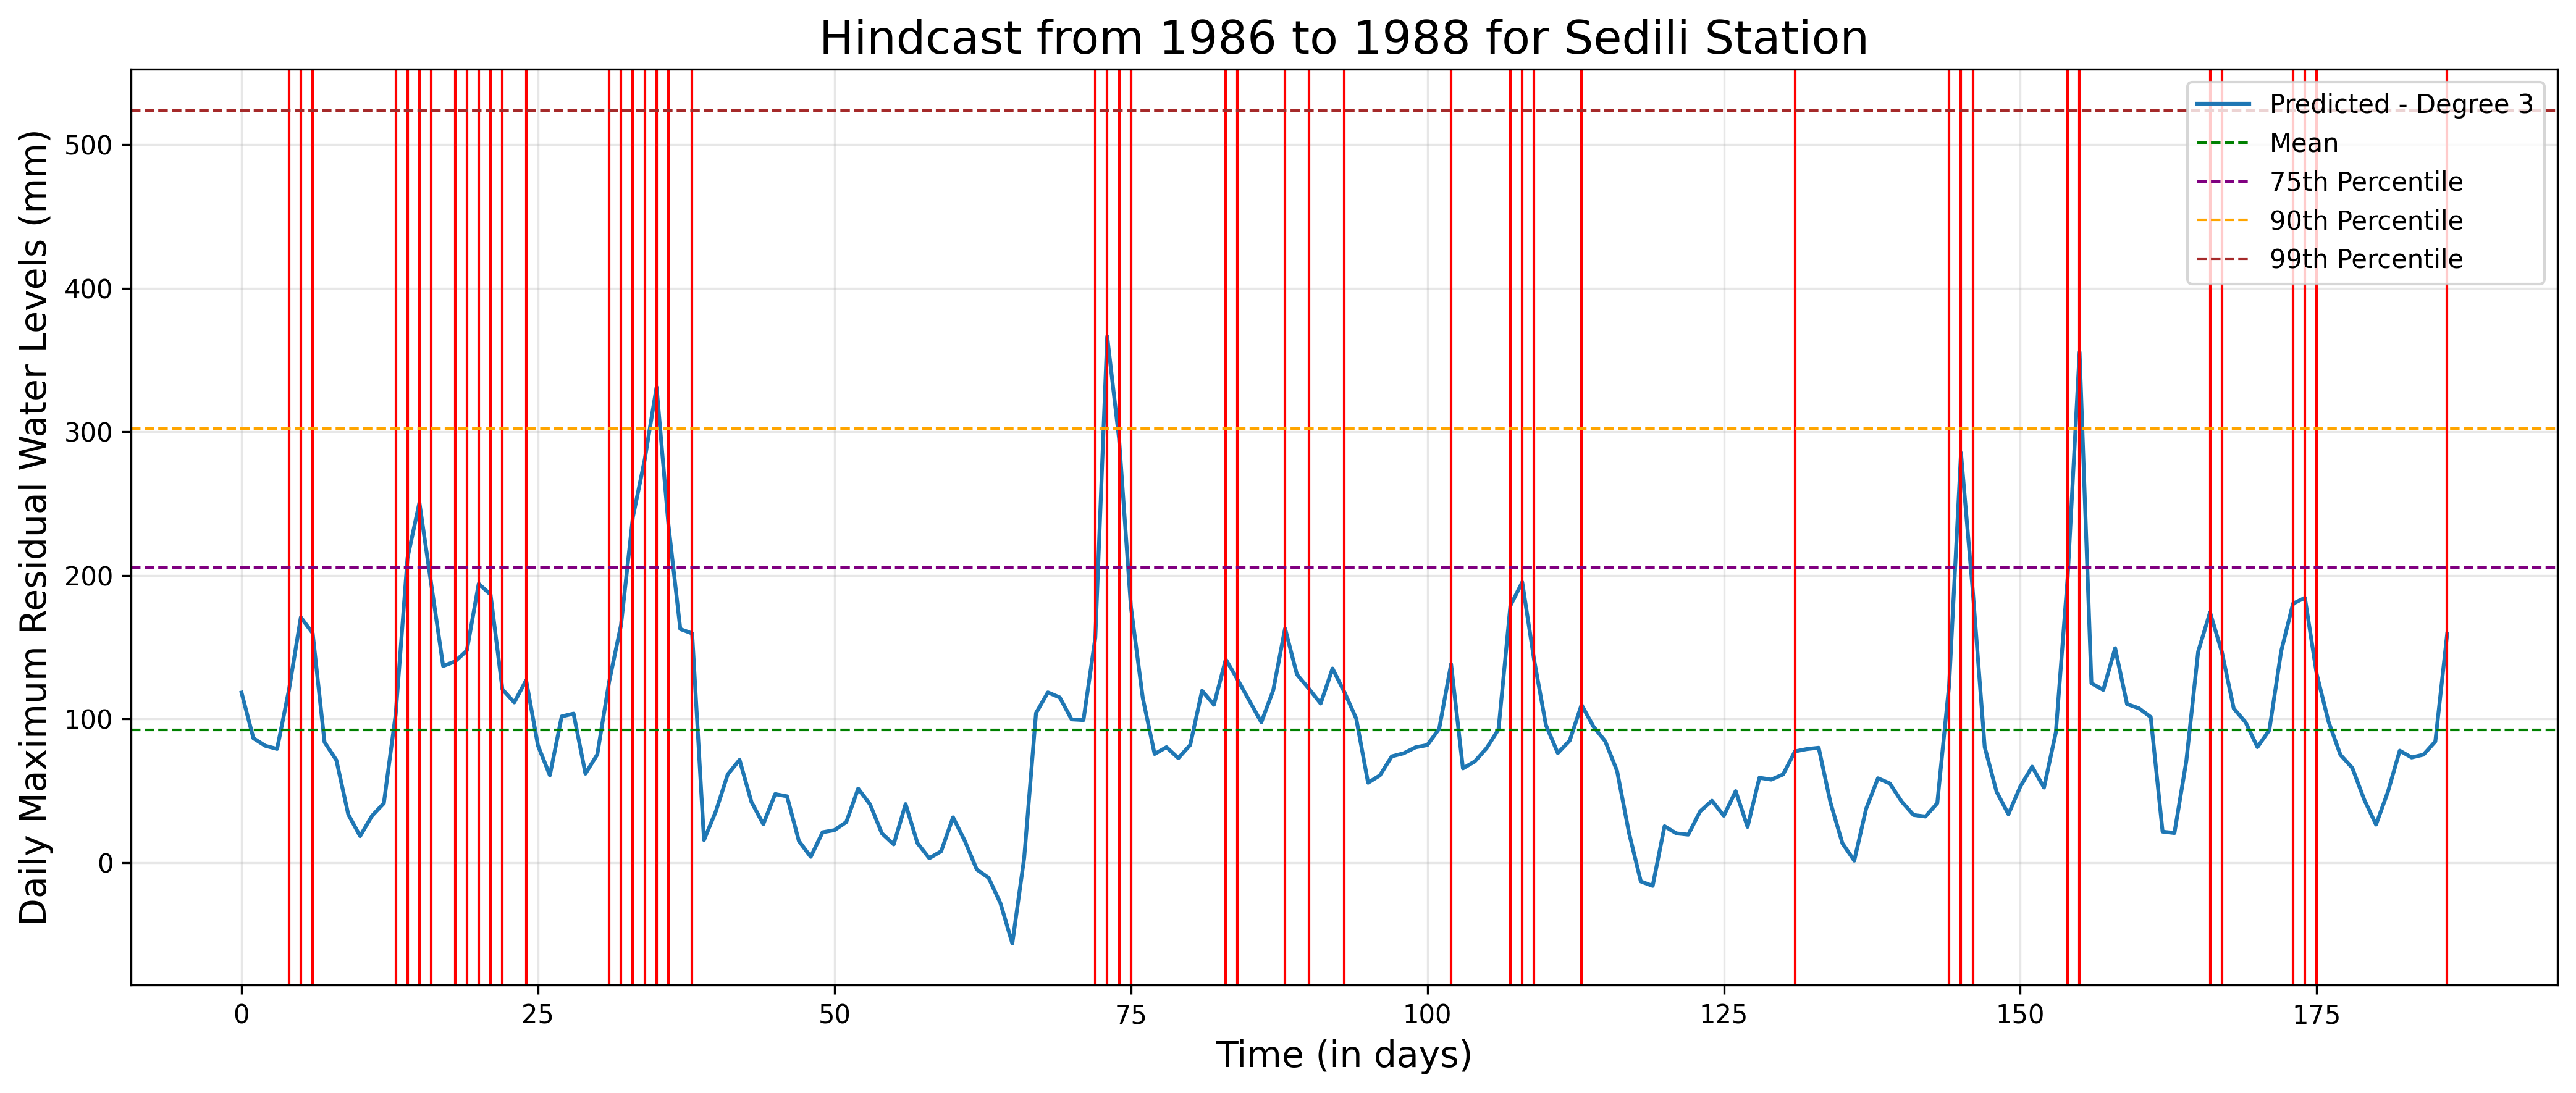
\includegraphics[width=0.9\linewidth]{Figures/HIndcast_1984_1986_sedili_SD.png}
        \caption{Hindcast for Sedili}
    \end{figure*}
    \item Tioman
        \begin{figure*}[htbp]
        \centering
        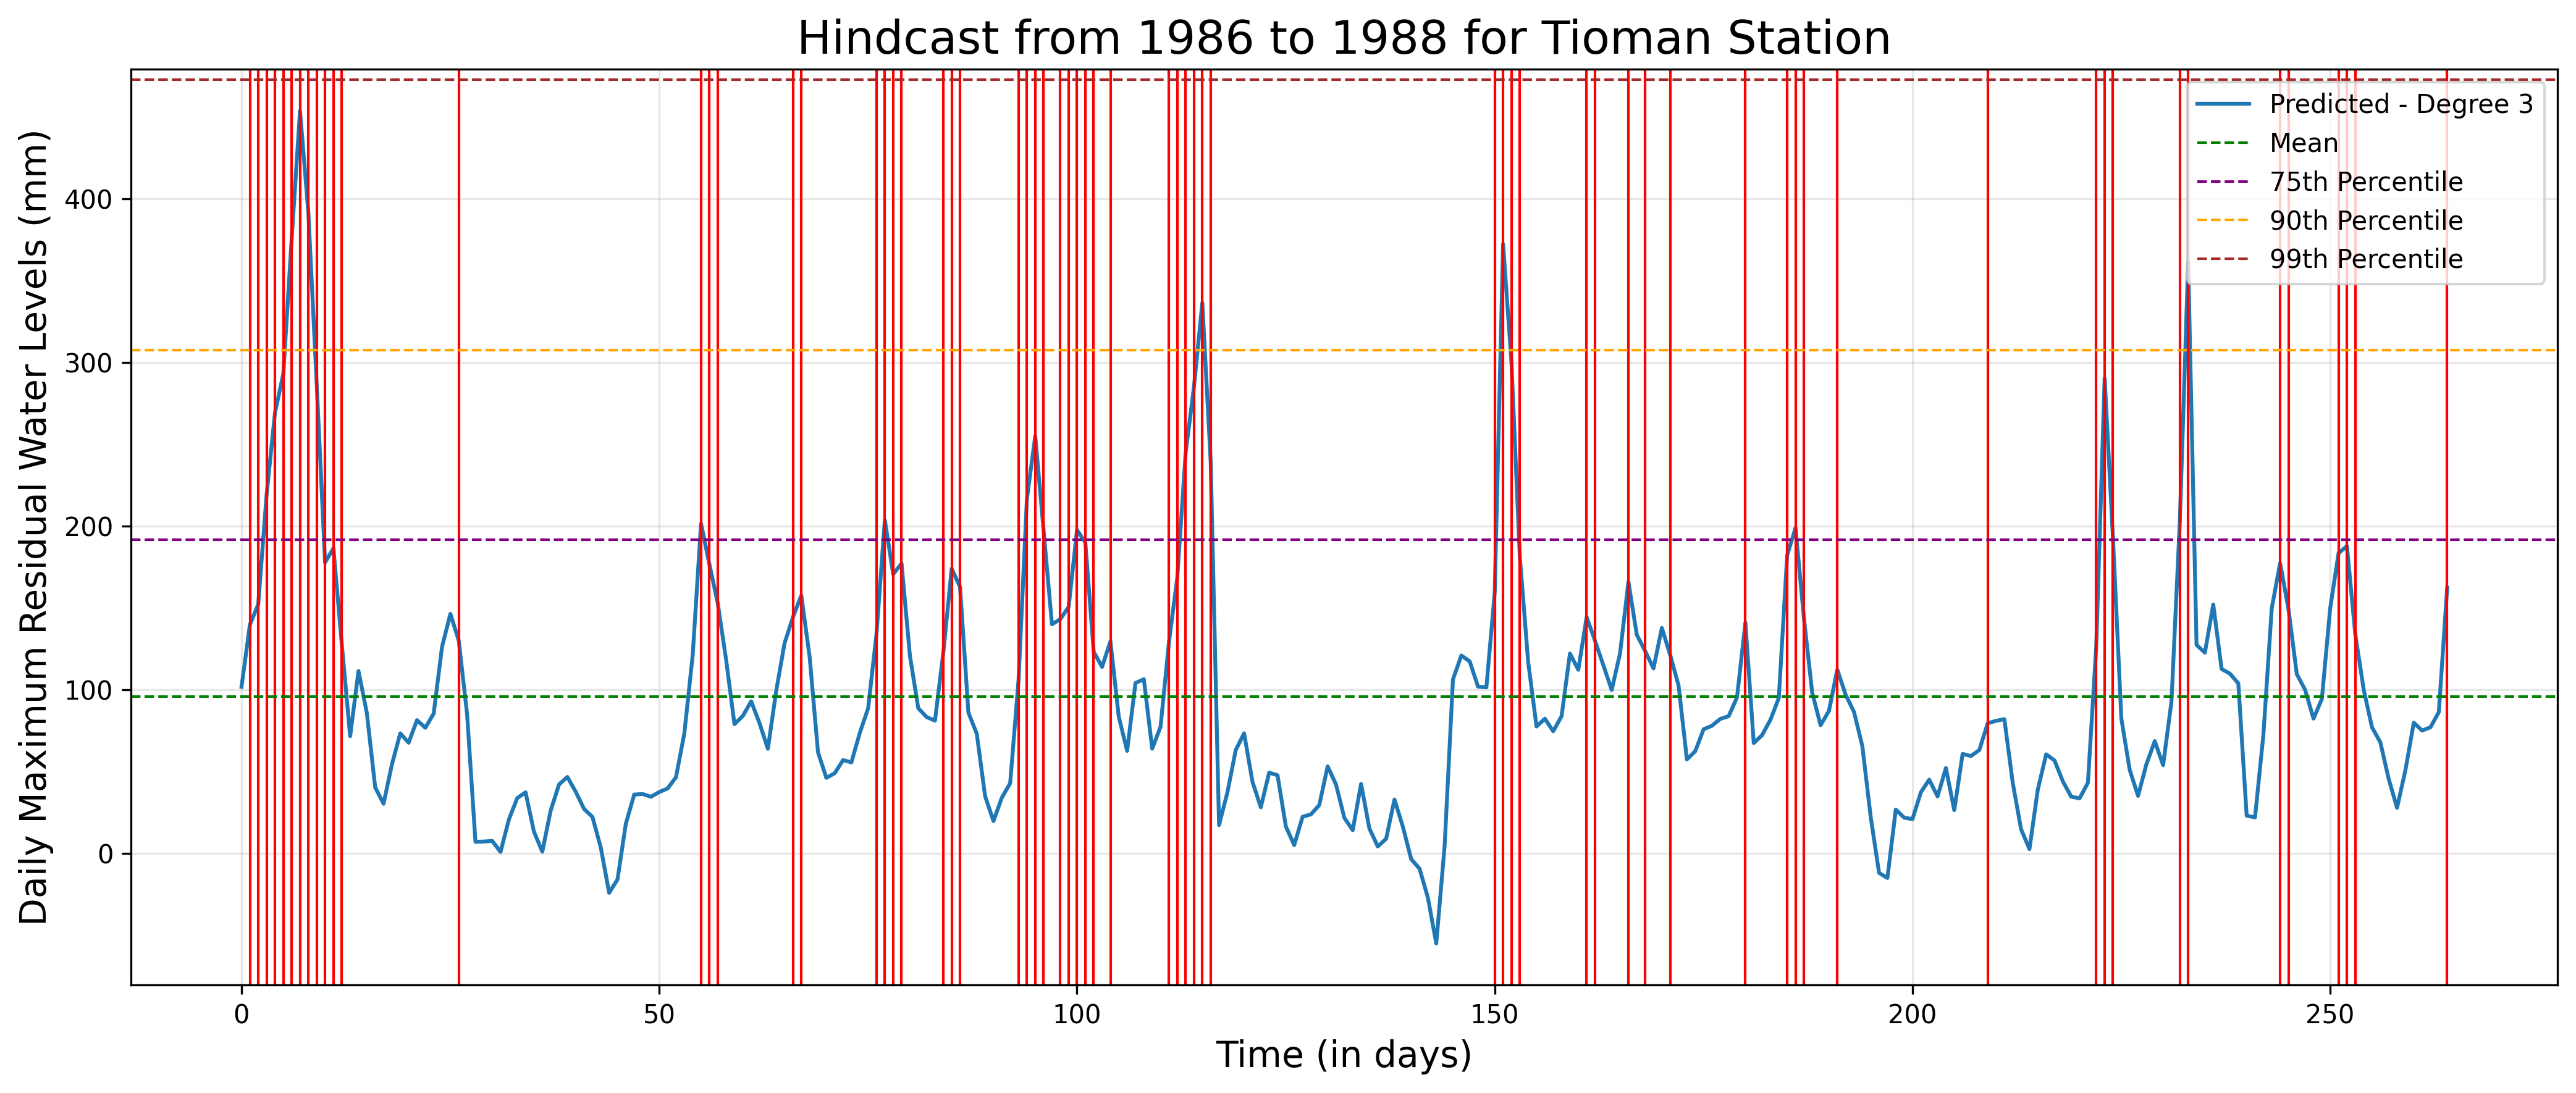
\includegraphics[width=0.9\linewidth]{Figures/HIndcast_1984_1986_tioman_SD.png}
        \caption{Hindcast for Tioman}
    \end{figure*}
    \end{itemize}
\end{itemize}
\end{document}